%% BioMed_Central_Tex_Template_v1.06
%%                                      %
%  bmc_article.tex            ver: 1.06 %
%                                       %

%%IMPORTANT: do not delete the first line of this template
%%It must be present to enable the BMC Submission system to
%%recognise this template!!

%%%%%%%%%%%%%%%%%%%%%%%%%%%%%%%%%%%%%%%%%
%%                                     %%
%%  LaTeX template for BioMed Central  %%
%%     journal article submissions     %%
%%                                     %%
%%          <8 June 2012>              %%
%%                                     %%
%%                                     %%
%%%%%%%%%%%%%%%%%%%%%%%%%%%%%%%%%%%%%%%%%


%%%%%%%%%%%%%%%%%%%%%%%%%%%%%%%%%%%%%%%%%%%%%%%%%%%%%%%%%%%%%%%%%%%%%
%%                                                                 %%
%% For instructions on how to fill out this Tex template           %%
%% document please refer to Readme.html and the instructions for   %%
%% authors page on the biomed central website                      %%
%% http://www.biomedcentral.com/info/authors/                      %%
%%                                                                 %%
%% Please do not use \input{...} to include other tex files.       %%
%% Submit your LaTeX manuscript as one .tex document.              %%
%%                                                                 %%
%% All additional figures and files should be attached             %%
%% separately and not embedded in the \TeX\ document itself.       %%
%%                                                                 %%
%% BioMed Central currently use the MikTex distribution of         %%
%% TeX for Windows) of TeX and LaTeX.  This is available from      %%
%% http://www.miktex.org                                           %%
%%                                                                 %%
%%%%%%%%%%%%%%%%%%%%%%%%%%%%%%%%%%%%%%%%%%%%%%%%%%%%%%%%%%%%%%%%%%%%%

%%% additional documentclass options:
%  [doublespacing]
%  [linenumbers]   - put the line numbers on margins

%%% loading packages, author definitions

%\documentclass[twocolumn]{bmcart}% uncomment this for twocolumn layout and comment line below
\documentclass{bmcart}

%%% Load packages
\usepackage{amsthm,amsmath}
\RequirePackage{natbib}

% Set image path for inserting figures
\usepackage{pstricks,pst-node}
\newcommand\measureISpecification{4ex}
\usepackage{graphicx}





%\RequirePackage[authoryear]{natbib}% uncomment this for author-year bibliography
%\RequirePackage{hyperref}
\usepackage[utf8]{inputenc} %unicode support
%\usepackage[applemac]{inputenc} %applemac support if unicode package fails
%\usepackage[latin1]{inputenc} %UNIX support if unicode package fails


%%%%%%%%%%%%%%%%%%%%%%%%%%%%%%%%%%%%%%%%%%%%%%%%%
%%                                             %%
%%  If you wish to display your graphics for   %%
%%  your own use using includegraphic or       %%
%%  includegraphics, then comment out the      %%
%%  following two lines of code.               %%
%%  NB: These line *must* be included when     %%
%%  submitting to BMC.                         %%
%%  All figure files must be submitted as      %%
%%  separate graphics through the BMC          %%
%%  submission process, not included in the    %%
%%  submitted article.                         %%
%%                                             %%
%%%%%%%%%%%%%%%%%%%%%%%%%%%%%%%%%%%%%%%%%%%%%%%%%


\def\includegraphic{}
\def\includegraphics{}



%%% Put your definitions there:
\startlocaldefs
\endlocaldefs


%%% Begin ...
\begin{document}

%%% Start of article front matter
\begin{frontmatter}

\begin{fmbox}
\dochead{Research}

%%%%%%%%%%%%%%%%%%%%%%%%%%%%%%%%%%%%%%%%%%%%%%
%%                                          %%
%% Enter the title of your article here     %%
%%                                          %%
%%%%%%%%%%%%%%%%%%%%%%%%%%%%%%%%%%%%%%%%%%%%%%

\title{Semi-supervised learning for integrative genomic analysis using hierarchical mixture models}

%%%%%%%%%%%%%%%%%%%%%%%%%%%%%%%%%%%%%%%%%%%%%%
%%                                          %%
%% Enter the authors here                   %%
%%                                          %%
%% Specify information, if available,       %%
%% in the form:                             %%
%%   <key>={<id1>,<id2>}                    %%
%%   <key>=                                 %%
%% Comment or delete the keys which are     %%
%% not used. Repeat \author command as much %%
%% as required.                             %%
%%                                          %%
%%%%%%%%%%%%%%%%%%%%%%%%%%%%%%%%%%%%%%%%%%%%%%

\author[
   addressref={aff1},                   % id's of addresses, e.g. {aff1,aff2}
   email={daniel.dvorkin@ucdenver.edu}   % email address
]{\inits{DD}\fnm{Daniel} \snm{Dvorkin}}
\author[
   addressref={aff1},                   % id's of addresses, e.g. {aff1,aff2}
   email={rani.powers@ucdenver.edu}   % email address
]{\inits{RKP}\fnm{Rani K.} \snm{Powers}}
\author[
   addressref={aff2},                   % id's of addresses, e.g. {aff1,aff2}
   email={michael.daniels@ucdenver.edu}   % email address
]{\inits{MWD}\fnm{Michael W.} \snm{Daniels}}
\author[
   addressref={aff2},                   % id's of addresses, e.g. {aff1,aff2}
   email={katerina.kechris@ucdenver.edu}   % email address
]{\inits{KK}\fnm{Katerina} \snm{Kechris}}

%%%%%%%%%%%%%%%%%%%%%%%%%%%%%%%%%%%%%%%%%%%%%%
%%                                          %%
%% Enter the authors' addresses here        %%
%%                                          %%
%% Repeat \address commands as much as      %%
%% required.                                %%
%%                                          %%
%%%%%%%%%%%%%%%%%%%%%%%%%%%%%%%%%%%%%%%%%%%%%%

\address[id=aff1]{%                           % unique id
  \orgname{Computational Bioscience Program, University of Colorado School of Medicine}, % university, etc
  \street{12801 E. 17th Ave.},                     %
  \postcode{80045}                                % post or zip code
  \city{Aurora},                              % city
  \cny{US}                                    % country
}
\address[id=aff2]{%
  \orgname{Department of Biostatistics and Informatics, Colorado School of Public Health},
  \postcode{80045}
  \city{Aurora},
  \cny{US}
}

%%%%%%%%%%%%%%%%%%%%%%%%%%%%%%%%%%%%%%%%%%%%%%
%%                                          %%
%% Enter short notes here                   %%
%%                                          %%
%% Short notes will be after addresses      %%
%% on first page.                           %%
%%                                          %%
%%%%%%%%%%%%%%%%%%%%%%%%%%%%%%%%%%%%%%%%%%%%%%

\begin{artnotes}
%\note{Sample of title note}     % note to the article
\note[id=n1]{Equal contributor} % note, connected to author
\end{artnotes}

\end{fmbox}% comment this for two column layout

%%%%%%%%%%%%%%%%%%%%%%%%%%%%%%%%%%%%%%%%%%%%%%
%%                                          %%
%% The Abstract begins here                 %%
%%                                          %%
%% Please refer to the Instructions for     %%
%% authors on http://www.biomedcentral.com  %%
%% and include the section headings         %%
%% accordingly for your article type.       %%
%%                                          %%
%%%%%%%%%%%%%%%%%%%%%%%%%%%%%%%%%%%%%%%%%%%%%%

\begin{abstractbox}

\begin{abstract} % abstract
\parttitle{First part title} %if any
Text for this section.

\parttitle{Second part title} %if any
Text for this section.
\end{abstract}

%%%%%%%%%%%%%%%%%%%%%%%%%%%%%%%%%%%%%%%%%%%%%%
%%                                          %%
%% The keywords begin here                  %%
%%                                          %%
%% Put each keyword in separate \kwd{}.     %%
%%                                          %%
%%%%%%%%%%%%%%%%%%%%%%%%%%%%%%%%%%%%%%%%%%%%%%

\begin{keyword}
\kwd{sample}
\kwd{article}
\kwd{author}
\end{keyword}

% MSC classifications codes, if any
%\begin{keyword}[class=AMS]
%\kwd[Primary ]{}
%\kwd{}
%\kwd[; secondary ]{}
%\end{keyword}

\end{abstractbox}
%
%\end{fmbox}% uncomment this for twcolumn layout

\end{frontmatter}

%%%%%%%%%%%%%%%%%%%%%%%%%%%%%%%%%%%%%%%%%%%%%%
%%                                          %%
%% The Main Body begins here                %%
%%                                          %%
%% Please refer to the instructions for     %%
%% authors on:                              %%
%% http://www.biomedcentral.com/info/authors%%
%% and include the section headings         %%
%% accordingly for your article type.       %%
%%                                          %%
%% See the Results and Discussion section   %%
%% for details on how to create sub-sections%%
%%                                          %%
%% use \cite{...} to cite references        %%
%%  \cite{koon} and                         %%
%%  \cite{oreg,khar,zvai,xjon,schn,pond}    %%
%%  \nocite{smith,marg,hunn,advi,koha,mouse}%%
%%                                          %%
%%%%%%%%%%%%%%%%%%%%%%%%%%%%%%%%%%%%%%%%%%%%%%

%%%%%%%%%%%%%%%%%%%%%%%%% start of article main body
% <put your article body there>

%%%%%%%%%%%%%%%%
%% Background %%
%%

\section*{Background}
\label{sec:intro}

Many investigations now involve the analysis of a large and growing range of genome scale data types, including 
DNA-sequence-derived variables, gene expression measurements, and epigenetic information. Each of these data  types can 
provide valuable information about the roles played by the genomic loci the data represent, but none by itself can provide a 
complete picture. The need for integrative approaches to realize the full potential of data growing in diversity as well as volume 
has been widely recognized over the last several years.  Several large-scale projects exist to  organize and make use of multiple 
data sources, and provide data and analysis tools for specific research domains  \citep{ENCODE2004a, ENCODE2012a, 
Celniker2009a, TCGAsite}. 

However, there is no generally agreed-upon methodology for integrative analysis and as the available data grow in size and 
complexity, so do the number and variety of questions we may wish to answer using that data. Recent reviews discuss some of 
the methodological challenges involved: large data sets consisting of heterogeneous data types, missing and incomplete data, 
noisy data from which it can be difficult to ascertain statistical significance, unclear relationships between the data types, and 
interpretability of results  \citep{Hamid2009a, Hawkins2010a}. An important conclusion is that integrated analysis is more 
effective than looking at data sources in isolation.
% In particular, simultaneous approaches are preferred to the sequential or filtering approach \citep{DeBie2005a, Hoffman2012a}.  
Simultaneous approaches provide more insight into the biological processes that generate the joint distribution of the data 
\citep{Lemmens2006a} and help reduce the effect of noise and increase power to detect signal \citep{Tyekucheva2011a}, and 
this is the approach we follow here.

In many studies, genomic data integration has focused on supervised \textbf{[REF]} classification approaches, which require 
high-quality training sets with both positive and negative controls.  When available training data sets are small, unreliable, or 
incomplete,  unsupervised methods are more commonly used\citep{Lemmens2006a, Xie2010a, Qin2011a, Hoffman2012a}.  
However, even  training data that are not suitable for supervised approaches can still provide valuable information.  In this work, 
we describe extension of the unsupervised methods first described in \citep{Dvorkin2013a} to allow the use of any available 
training data, no matter how small or incomplete, for semi-supervised learning.

Here we focus on a gene-centric approach,  where data from genes and their cis-regulatory regions can be used to identify 
genes that play key roles in particular processes and phenotypes. Although there are a variety of applications,  such as predicting 
genes relevant to a certain disease or pathway [REF], we focus on  predicting gene essentiality. Essential genes are required for 
the survival of an organism and are important to understand the basic principles of cellular function, to engineer microorganisms 
using synthetic biology, and to identify potential targets for antibiotics \citep{Zhang2015a, Juhas2011a}. A variety of 
experimental methods 
%are used including saturation transposon mutagenesis, antisense RNA inhibition and single-gene-specific mutagenesis [PMID: 26857942, PMID: 21889892] 
and many of these results are collected in databases such as DEG and OGEE \citep{Lou2014a,Chen2012}.  Although 
primarily focused on model organisms such as bacteria and yeast, more recent methods have studied gene essentiality in 
humans using CRISP-R and gene trapping methods \citep{Wang2015a}. Because of the expense and labor involved with the 
experimental approaches, computational methods have been used to predict essential genes, and machine learning methods 
which rely on training a classifier using examples of essential genes have become a common strategy  \citep{Mobegi2017,Zhang2016a}. 
Several features have been used to predict essential genes including both features of the DNA sequence such as GC content, and predicted 
features of the translated proteins such as hydrophobicity. All of the features may be expected to be 
have predictive value for essentiality, but none are particularly strong predictors. By  combining these measures, the hope is to 
predict essential genes with a much higher degree of accuracy than would be possible  with any one measure alone.

Alexandridis et al. \citep{Alexandridis2004a} describe an ad hoc method for semi-supervised mixture modeling with incomplete training data.  In Section \ref{sec:methods}, we build on their work and the more rigorous approach of \citep{Elkan2008a} to develop semi-supervised hierarchical mixture models for any type of training data, specifically designed to deal with the case when only positive examples such as known essential genes are available, often called ``positive unlabeled learning'' or PUL \citep{He2010a}.  A mixture model for a single data source is described, followed by a hierarchical mixture model when there are multiple data sources. Then Sections \ref{sec:simulation} and \ref{sec:application} show that the inclusion of positively labeled samples in a semi-supervised learning framework improves our ability to detect genes of interest.  We also show that our method outperforms other methods for PUL that are based on standard supervised learning approaches. Although our case study is on gene essentiality, our framework is general for any gene-centric problem with multiple data types and when there is a small set of positive labels.

\section*{Methods}
\label{sec:methods}
We use a generative mixture model approach to represent classes of genes such as target vs. nontarget and essential vs. nonessential, with a hierarchical structure to represent different types of data and the relationships between them.  Mixture models have a long history and a rigorous statistical framework for inference and prediction \textbf{REFERENCES}. Hierarchical mixture models have been applied in other contexts \citep{Vermunt2005a} and in a variety of bioinformatic applications \citep{Jornsten2008a, Li2010a}. In this work, we examine models that are tree-structured directed acyclic graphs, in which the nodes represent random variables, which may be hidden or observed, and the edges represent the conditional dependence structure of the variables. This approach allows for simultaneous modeling of a wide range of data sources, with computationally efficient model fitting and easily interpretable results. We first describe the semi-supervised method for single mixture models and then extend that to hierarchical mixture models for data integration.

\subsection*{Single Mixture Model}
\label{subsec:methods.unsup.marginal}

A \textit{generative} mixture model arises when we wish to model the distribution of one random variable $X$ which 
depends on the value of another random variable $Y$, so we say that $Y$ \textit{generates} $X$. We assume $Y$  is a 
univariate categorical random variable that can take on one of $K$ categories (1,\ldots, $K$), while $X$, which may be 
multivariate, can have any distribution. For notational compactness, let $f_y( x) = f( x | Y = y)$, and $f(x) = \sum_k p_k f_k( x) \ , k = 1, \ldots, K.$
%\begin{equation}\label{eqn:methods.marginal_mixture_model}
%	\textstyle f(x) = \sum_k p_k f_k( x) \ , k = 1, \ldots, K.
%\end{equation}
We also assume we observe $X$, but not $Y$---that is, $Y$ is \textit{hidden}.
In our examples, typically $K=2$, for example ``non-essential" versus ``essential."  The 
model may also be represented graphically, as shown in \textbf{COMBINE MARGINAL AND HIERARCHICAL FIGURE?}. Our challenge is to infer the parameters $\theta$ (e.g., Gaussian mean and variance for each mixture component), which 
will allow us to calculate expected values for these hidden states.  The joint density of $X$ and $Y$ is therefore
%\begin{equation}\label{eqn:f_x_y_normal_mixmod}
$	f( x, y | \theta) = p_y \ f_y( x | \theta)$.

From this, for a sample $ X = ( x_1, \ldots,  x_N)$, we use the EM algorithm \citep{Dempster1977a, McLachlan2008a} to 
estimate the parameters and find the posterior probabilities $\hat w_{n,y} = P(y_n = y |  x_n, \hat\theta)$.  Specifically, 
the EM algorithm finds the maximum likelihood estimate $\hat\theta$ by iterative maximization of the ``Q-function,'' or the 
conditional expected log-likelihood
\begin{equation}
\label{eqn:qfun.defn}
	\textstyle Q(\theta|\theta^{(i-1)}) = E_{Y}\left[ \sum_n \log f( x_n, y_n | \theta) \ | \  X, \theta^{(i-1)}\right]
\end{equation}
where $\theta^{(i-1)}$ is the previous iteration's $i$ estimate for the parameters.  For the model,
\begin{equation}\label{eqn:qfun_mixmod}
	Q(\theta|\theta^{(i-1)})= \textstyle \sum_{n,k} w_{n,k} \{\log p_k + \log f_k( x_n | \theta^{(i-1)})\}
\end{equation}
where
\begin{equation}\label{eqn:w_n_y_mixmod}
	w_{n,y} \ = \ P(y_n = y |  x_n, \theta^{(i-1)}) \ = \ \frac{p_y^{(i-1)} f_y( x_n | \theta^{(i-1)})}{\sum_k p_k^{(i-1)} f_k( x_n | \theta^{(i-1)})}.
\end{equation}
Generally, $w_{n,1}$ is the posterior probability that $y_n = 1$ given the data.  In the problems at hand, $w_{n,1}$ is the posterior probability that gene $n$ is in the more ``interesting'' category given the particular data source being used.

Depending on the data type and the distribution, different functional forms for $f$ may be appropriate (e.g., discrete, continuous). In addition within a data type, different alternatives may be available.  For example, 
the Gaussian may be compared to a longer tailed distribution like the Pearson's VII or the Poission distribution may be 
compared to the negative binomial \citep{Dvorkin2013b}. For model selection among forms of $f$, we use the ICL-BIC (integrated complete likelihood Bayesian information 
criterion) \citep{Biernacki2000a}.  See Supplementary Material for more details.

\subsection*{Training Data}

When training labels are available for some of the samples---for example, we know a number of essential genes in \textit{S.\ cerevisiae} ---we may wish to incorporate this information into the estimation procedure.   The authors in \citep{Alexandridis2004a} describe a method for the standard categorical mixture models, which we refer to here as the single mixture model:  briefly, at the end of each E-step, update the posterior probabilities for the labeled samples based on their labels.  For example, if the $n$th gene is known to be in category 1 ($y_n = 1$) then we would set $w_{n,1} = 1$ and $w_{n,k} = 0 \ \forall \ k \neq 1$, regardless of the values of $(w_{n, 1}, \ldots, w_{n,K})$ calculated previously.  However, this method  does not extend well to models with multiple data sources.  \citep{Elkan2008a} present a more principled approach of incorporating training data into the model as an additional type of observed data, which they apply in a support vector machine (SVM) context.  Here we apply their approach in a mixture model context to extend both the single and hierarchical mixture models, with an emphasis on the positive unlabeled learning (PUL) context in which only positive examples are known.

\subsection*{Single Mixture Model: Semi-Supervised Method}\label{subsec:methods.semisup.marginal}

In the presence of partial training data, such as when only a few positive labels are known, define a new random variable, 
$T$, to represent the training labels, in addition to the observed data $X$ and hidden states $Y$.  $T$ is a 
categorical random variable that can take on the values from $1, \ldots, K^{trn}$, where $K^{trn} = K+1$. If the training 
label is known for an observation, then $T \leq K$. When the training label  is unknown for an observation, then $T = K
^{trn}$, which is always the case in the unsupervised model. In other words, $P(Y = T | T \leq K) = 1$ 
always, while $P(Y = y | T = K^{trn})$ is a free parameter to be estimated.  Let $\vec R^{trn}$ be the $K
^{trn} \times K$ matrix such that $r_{t,y}^{trn} = f(y | t) = P(Y = y | T = t)$, and observe that the top 
$K$ rows of $\vec R^{trn}$ are fixed at $\vec I_K$, the $K \times K$ identity matrix, while the $K^{trn}$th row is free:
\begin{equation}\label{eqn:Rtrain}
	\vec R^{trn} = \begin{pmatrix}
		1 & \cdots & 0 \\
		\vdots & \ddots & \vdots \\
		0 & \cdots & 1 \\
		r_{K^{trn}, 1}^{trn} & \cdots & r_{K^{trn}, K}^{trn}
	\end{pmatrix}
\end{equation}
subject to the constraint $\sum_k r_{K^{trn}, k}^{trn}= 1$.  In contrast to fully supervised learning methods, this formulation 
allows us to estimate parameters using information from both labeled and unlabeled samples simultaneously, and also to 
make use of label information when only positive labels are available.  We show in Section \ref{sec:simulation} that this 
approach can significantly improve the performance of the model.

We incorporate the labels into the model as the sample $\vec t = (t_1, \ldots, t_N)$.  For example, for our example application ($K = 2$ for ``essential'' or ``non-essential''), we may have some genes known to be essential  while others are of unknown binding status.   Then for $m,n \in \{1, \ldots, N\}$,  $t_m = 1$ when we know that the $m$th gene is essential, while $t_n = 3$ when the status of the $n$th gene is unknown.  If we knew the $m$th gene to be \textit{un}essential, we would have $t_m = 
2$, but our analysis here does not consider the case of labeled negative samples.  Conceptually, $Y$ generates both $T$ 
and $X$; those samples for which $T \leq K$ may be thought of as samples for which $Y$ is observed rather than hidden.  
We assume the values of $T$ are accurate, that is, there are no unlabeled samples.  The model is illustrated graphically in 
Figure \ref{fig:methods.marginal.semisup} \textbf{[NEW FIGURE]}.

However, because of the fixed relationship between $Y$ and $T \leq K$, it is more practical to perform most of the 
calculations on the model as though $T$ generated $Y$.  To obtain $\hat{\vec R}^{trn}$, we need only find the MLE for the 
$K^{trn}$th row of $\vec R^{trn}$, that is, $\hat{\vec r}_{K^{trn}}^{trn} = (\hat r_{K^{trn},1}^{trn}, \ldots, \hat r_{K^{trn},K}
^{trn})$.   The joint density of all variables in the model is

\begin{equation}\label{eqn:methods.f_t_x_y_semisup_mixmod1}
	f(t, \vec x, y | \theta) = p(T=t) p(Y=y|T=t) p(X=x| Y=y,T=t)
\end{equation}
\begin{equation}\label{eqn:methods.f_t_x_y_semisup_mixmod2}
	f(t, \vec x, y | \theta) = p_t^{trn} \ r_{T,t}^{trn} \ f_y(\vec x | \theta).
\end{equation}
where $p_t^{trn} = P(T = t)$, and the Q-function is
\begin{equation}\label{eqn:methods.semisup_marginal_qfun}
	\begin{array}{rcl}
		Q(\theta|\theta^{(i-1)})  & = & \sum_{n, k^{trn}} t'_{n,k^{trn}} \log p_{k^{trn}}^{trn} \\&& + \sum_{n, k^{trn}, k} 
		t'_{n,k^{trn}} w_{n,k} \log r_{k^{trn},k}^{trn} \\&& + \sum_{n,k} w_{n,k} \log f_k(\vec x_n).
	\end{array}
\end{equation}
Here $t'_{n,t} = I(t_n = t)$, and after some simplification, the central calculation for the E-step is
\begin{equation}\label{eqn:methods.w_n_y_semisup_mixmod}
	w_{n,y} \ = \ P(y_n = y | t_n, \vec x_n, \theta^{(i-1)}) \ = \ \frac{r_{t_n,y}^{trn (i-1)} \ f_y(\vec x_n | \theta^{(i-1)})}
	{\sum_k r_{t_n,k}^{trn (i-1)} \ f_k(\vec x_n | \theta^{(i-1)})}.
\end{equation}
The modeling of the observed data is the same as in the unsupervised case. By default, labeled samples are given the same weight as unlabeled samples in the parameter estimations.  However, if we  have a small training sample, we may choose to assign a higher weight $w^{trn}$ to labeled samples.  Please see the supplementary material for selection of weights.

 
 \subsection*{Hierarchical Mixture Models}

The previous model describes the case when there is only a single data type (e.g., one normally distributed 
variable) or a multivariate distribution of the same type (e.g.,  multivariate normal). But for many integration problems, as with 
predicting essential genes, data sets may need to be grouped by distribution type (e.g., continuous or discrete) and 
measurement type (e.g., expression levels or binding information). For example, there are binary variables such as location information (e.g., is the predicted subcellular location of the corresponding protein in the nucleus) or continuous variables like expression \textbf{TABLE}. We present a hierarchical mixture model extending the 
framework above for any number and types of genomic level data.
%Here a a top-level hidden categorical variable generates intermediate hidden categorical variables, which in turn generate the observed data. The top-level variable represents the general status of genes as interesting (such as essential genes in Saccharomyces) while the intermediate variables represent more specific classifications, such as bound vs. unbound. We can then estimate the parameters of the model simultaneously, taking into account all observed data and the relationships between the data types. The hierarchical mixture modeling approach helps us form a more complete picture of these relationships and how they contribute to the overall classification.  

At the top of the hierarchies shown in \textbf{Figure \ref{fig:methods.topology.semisup}} is the hidden categorical random 
variable $Y_0$, which takes on integer values from 1 to $K_0$ for some integer $K_0 > 1$.  In the problems at hand, we assume 
$K_0 = 2$ always and $Y_0 = 1$ corresponds to ``interesting'' genes.  Next, let $Z$ denote the number of data sources, and $z 
\in \{1, \ldots, Z\}$ denote the $z$th data source.  The intermediate hidden categorical random variables $Y_z$ take on integer 
values from 1 to $K_z$ for some integer $K_z > 1$.  The distributions of the $Y_z$'s depend---directly or indirectly, depending 
on the model topology---on the value of $Y_0$.  Also define the observed random variables $X_1, \ldots, X_Z$ (each $X_z$ may 
be multivariate) where the distribution of $X_z$ depends only on the value of $Y_z$.  That is, each $X_z$ is generated by $Y_z$.   
For example, in the \textit{Saccharomyces} data, $Z = 14$ with each value of $z$ corresponding to a different sequence-derived 
measure. Each $Y_0$ generates $Y = (Y_1, \ldots , Y_Z )$. This model treats all observed variables as equally important to 
estimating the distribution of $Y_0$. We have explored alternative conditional relationships among the $Y$'s in 
\citep{Dvorkin2013b}.

Given $N$ genes, for $n = 1, \ldots, N$ the estimated posterior probability that the $n$th gene is of interest is $P(y_{0,n} = 1 
| \vec x_{\cdot,n}, \hat\theta)$.  Here $y_{0,n}$ is the $n$th hidden status variable, that is, a realization of $Y_0$.  
Similarly, $y_{z,n}$ is the hidden realization of $Y_z$ for the $n$th gene, and $\vec x_{\cdot,n} = (\vec x_{1,n}, \ldots, \vec 
x_{Z,n})$ is the observed data for the $n$th gene, with $\vec x_{z,n}$ being a realization of $X_z$.  Finally, $\hat\theta$ denotes 
the estimated parameters of the model.   See the supplementary material for full details of the estimation procedure. 
Briefly,  the first step in the hierarchical model fitting is to fit a single mixture model to each data source, as described in Section \ref{subsec:methods.unsup.marginal}, to choose the number  f components $K_z$ and marginal distribution which will be used for that data. These steps follow the EM algorithm described above, and are used for initialization; the individual model fits can be updated in the full algorithm. Then after the marginal distributions are selected, this is used for initialization of the EM algorithm for the full model. The E-step consists of finding the posterior probabilities, given the data and current iteration of $\theta$, for the hidden states $Y_z$ for all data sources $z$, and for the primary hidden state $Y_0$.  The M-step is a straightforward maximum likelihood estimation for and the parameters $\theta$, the marginal distribution of $P(Y_0=y_0)$, and conditional relationships among the hidden variables $P(Y_z = y_z| Y_0 = y=0)$. More details are provided in the Supplementary Material.





 
 
\subsubsection*{Sub-sub heading for section}
Text for this sub-sub-heading \ldots
\paragraph*{Sub-sub-sub heading for section}
Text for this sub-sub-sub-heading \ldots
In this section we examine the growth rate of the mean of $Z_0$, $Z_1$ and $Z_2$. In
addition, we examine a common modeling assumption and note the
importance of considering the tails of the extinction time $T_x$ in
studies of escape dynamics.
We will first consider the expected resistant population at $vT_x$ for
some $v>0$, (and temporarily assume $\alpha=0$)
%
\[
 E \bigl[Z_1(vT_x) \bigr]= E
\biggl[\mu T_x\int_0^{v\wedge
1}Z_0(uT_x)
\exp \bigl(\lambda_1T_x(v-u) \bigr)\,du \biggr].
\]
%
If we assume that sensitive cells follow a deterministic decay
$Z_0(t)=xe^{\lambda_0 t}$ and approximate their extinction time as
$T_x\approx-\frac{1}{\lambda_0}\log x$, then we can heuristically
estimate the expected value as
%
\begin{eqnarray}\label{eqexpmuts}
E\bigl[Z_1(vT_x)\bigr] &=& \frac{\mu}{r}\log x
\int_0^{v\wedge1}x^{1-u}x^{({\lambda_1}/{r})(v-u)}\,du
\nonumber\\
&=& \frac{\mu}{r}x^{1-{\lambda_1}/{\lambda_0}v}\log x\int_0^{v\wedge
1}x^{-u(1+{\lambda_1}/{r})}\,du
\nonumber\\
&=& \frac{\mu}{\lambda_1-\lambda_0}x^{1+{\lambda_1}/{r}v} \biggl(1-\exp \biggl[-(v\wedge1) \biggl(1+
\frac{\lambda_1}{r}\biggr)\log x \biggr] \biggr).
\end{eqnarray}
%
Thus we observe that this expected value is finite for all $v>0$ %(also see \cite{koon,khar,zvai,xjon,marg}).
%\nocite{oreg,schn,pond,smith,marg,hunn,advi,koha,mouse}

\section*{Application to Data}

\subsection*{Methods}

\subsubsection*{Feature Description}\label{subsubsection:feature}\
Identifying essential genes that is, genes without which the organism cannot survive in the yeast Saccharomyces cerevisiae  \citep{Seringhaus2006a} and related species has been an area of investigation. Several features have been used to predict essential genes including both features of the DNA sequence such as GC content, and predicted features of the proteins translated from the genes such as hydrophobicity and subcellular localization. All of the features may be expected to be have predictive value for essentiality, but none are particularly strong predictors. By combining these measures, the hope is to predict essential genes with a much higher degree of accuracy than would be possible with any one measure alone.
  
To predict essentiality of the genes in yeast Saccharomyces cerevisiae, our analysis uses features associated with each gene from two sources: 1) fourteen sequence-derived features from the Seringhaus, et al., 2006 study, and 2) eight additional features from the Ensembl website \citep{Ensembl2018}. We added new features to check how sensitive the results were to the feature set. Feature definitions are listed in Table \ref{tab:methods.training.variables}. Three of 22 features (vacuole, in how many of 5 proks blast, and intron) were removed from the analysis due to low content (less than 5\% of non-zero values). At lower training sizes, their low content resulted in deterministic models because the randomization employed multiple seeds until the design matrix had no columns of zeroes. Genes which had values for this low-content features would have been selected more frequently than genes without information in these features.

\subsubsection*{Cross-Validation Strategy}\label{subsubsection:cv}\
In the unsupervised simulation, semi-supervised was compared against the unsupervised method described in Dvorkin et. al., \citep{Dvorkin2013a}. The unsupervised method utilizes both K-means and C-means clustering in a Bayesian Belief Network to classify essentiality of the genes in Saccharomyces cerevisiae. We trained our methods from the set of 769 essential genes (positive labels) of the total 3500 genes. Additionally, we contrasted all 22 features against a subset of 14 sequenced-derived features as predictors of essentiality. Training set sizes were based on increments of 5 with minimum set sizes greater than the number of features to prevent rank deficiency in training sets. Iterations (n=30) were used to average the AUC or other metrics used to evaluate performance. 

The cross-validation strategy for the supervised case incorporates an unbalanced strategy to the test set \ref{tab:methods.training.variables} along with a contamination rate. For an unbalanced design, test sets utilize the remaining genes not used in the training sets rather than a balanced strategy which matches training and testing set sizes. The unbalanced strategy was chosen because, in practice, an investigator would typically want to test all the remaining genes for essentiality rather than just a subset of genes. Another concept interwoven into the analysis is contamination. Contamination considers the dilemma from falsely assigned genes in the training sets. The semi-supervised and unsupervised methods do not consider negative labels in their computations and, thus, are unaffected by contamination. For supervised methods, positive labels in the training set are mixed with negative labeled genes for analysis when varying percentages of contamination are introduced. 

In the supervised simulation, semi-supervised was compared against three supervised methods (LASSO, SVM, and Random Forest) at low training set sizes. AUC performance of these four methods was compared across training set sizes between 1\% (n=35) and 10\% (n=350) from all 3500 genes. Genes randomly chosen for the supervised training sets reflect the same ratio of positive and negative labels as seen in the full data set. Among the 3500 yeast genes, there are 769 essential genes resulting in a 21\% ratio. Therefore, as an example, at 1\% training size, 35 randomly chosen genes contained 7 positive labels (21\% of 35) and 28 negative labels for supervised methods, while semi-supervised methods analyzed 35 positively labeled genes. In order to mimic contamination, negative labels were reassigned a positive label at rates of 0\%, 20\%, and 50\%. 

For all results, unique initial seeds were chosen based on the iteration number, training set size, and contamination (for supervised comparison only). Iterations were increased to 100 to better discriminate effects at low training sets. Once the cross-validation data was generated by a seed, the same data was used to compare each method.  

\subsubsection*{Algorithms}\label{subsubsection:algorithm}\
All simulations were performed in R version 3.3.3. The semi-supervised and unsupervised analysis utilized functions from the lcmix package. The lcmix package developed and implemented in the previous paper by Dvorkin, Biehl, and Kechris \textbf{A Graphical Model Method for Integrating Multiple Sources of Genome-scale Data} \citep{Dvorkin2013a} and can be downloaded from http://r-forge.r-project.org/projects/lcmix/. LASSO was performed using the glmnet command in the glmnet package \citep{Friedman}. Using cv.glmnet, k-fold cross validation optimized the minimum lambda for the LASSO function. SVM analysis used the svm command under the e1071 package \citep{Meyer}. Various runs using different criteria revealed a radial kernel density and C-classification optimized AUC performances. Random Forest was performed with the randomForest command under the randomForest package \citep{Liaw} All supervised predictions used the predict command in the stats package. 

\subsubsection*{Performance}\label{subsubsection:performance}\
The AUC mean, variance, and CV (median absolute deviation/median) of the three supervised methods were contrasted against semi-supervised method. Because LASSO outperformed the other supervised models in AUC across all training set sizes and contamination rates, a closer evaluation of its performance was compared with semi-supervised method. In order to fairly contract LASSO performance to semi-supervised, the prediction scores were re-scaled to be between 0 and 1. Precision, recall, and f-measure further discriminated the two methods with four rescaled prediction score cutoffs including the median and prediction scores of 0.5, 0.8, and 0.95. The median cutoff is a relative measure based on the data while the other three cutoffs are absolute. The f-measure was calculated from the average precision and recall at each training set size from 1\% to 5\%.

\subsection*{Results}\label{subsection:results}\
We describe each of the features used in the analysis along with their associated distributions based on their data types and the optimized determined \textbf{K}, univariate prediction classes, in predicting essentiality for each one in Table \ref{tab:definition}. Based on the range of univariate estimated AUCs (0.494-0.674), many of the features have low predictive value on their own but in the following comparisons we will explore their combined predictive power. We used cross-validation simulations to compare our hierarchical mixture model semi-supervised method with unsupervised and supervised methods. We hypothesize that semi-supervised method outperforms both unsupervised methods at any training set size and supervised methods at low training set sizes especially when positive labels are contaminated.

\subsubsection*{Unsupervised Comparison}\label{subsubsection:unsupervised.compare}\
The complete essentiality data for Saccharomyces cerevisiae contains n=769 positive labeled genes. To explore whether our conclusions were sensitive to the choice of features, we first used only 14 sequence-derived features from  Seringhaus and then a larger set of 22 features, which included the Seringhaus features and eight additional features collected from Ensembl (see Methods). Semi-supervised performs better than unsupervised for AUC regardless of predicting with 14 sequence-derived or all 22 features or training set size (Figure \ref{fig:unsup}). The AUC variance for both methods increases as training size increases when training on all essential genes. This is expected as the test set is relatively larger and more constant with the smaller training sets. The eight additional features added from Ensembl Biomart generally improves AUC performance and decreases variance for both methods.

\subsubsection*{Supervised Comparison}\label{subsubsection:supervised.compare}\
Next, we compared the semi-supervised method with a supervised strategy using all essential genes for the training set and all 22 features. Supervised algorithms require both positive and negative labels. Therefore, we picked a random set of the non-essential genes to be the negative labels (Figure \ref{fig:diagram}), but also included some contamination (some essential genes labeled as negatives in the training set) since in practice, the complete set of negative labels will not be known in many situations.  

LASSO and semi-supervised outperforms the other two supervised methods - SVM and Random Forest (Figure \ref{fig:AUCboxplots}). At low training sizes (i.e., 2\%, n = 70), semi-supervised method has a higher mean AUC than the three supervised methods. LASSO does not match the stability (lower variance) of semi-supervised until around 5\% (n=175) training set size. However, for larger training set sizes, the AUC variance of semi-supervised increases while variance from LASSO slightly decreases. As contamination increases, all three supervised methods decrease in performance. At 50\% contamination, semi-supervised method bests all methods across all training set sizes (up to 10\%). The CV (median absolute deviance/median) for semi-supervised is lower than LASSO across all contamination levels and training set sizes up to 5\% (Figure \ref{fig:AUCsummarymedian}).

\subsubsection*{Semi-supervised versus LASSO Performance}\label{subsubsection:performance.compare}\
To compare the best performing supervised method, LASSO, for our data to semi-supervised method, prediction scores were rescaled to be between 0 and 1. At 1\% training level, LASSO kernel densities of prediction scores exhibit an unimodal distribution while semi-supervised methods exhibit  bi- or multi-modal behaviors (Figure \ref{fig:hist}). Uni-modal behavior makes it more difficult to find better separation of gene types (e.g., essential versus non-essential). As training level increases, LASSO kernel densities of prediction scores continue to exhibit unimodal distributions while semi-supervised methods maintain their multimodal behaviors.  

Focusing on 0\% contamination in Figure \ref{fig:perf0}, the three absolute cutoffs (50\%, 80\%, and 95\%) reveal a higher recall across all training set sizes for semi-supervised and the median cutoff shows semi-supervised outperforming LASSO up to 3\% at which they become comparable. Also, up to 3\%, semi-supervised outperforms LASSO in precision at the median cutoff. Precision generally increases as the absolute cutoff increases with LASSO besting semi-supervised as training set size increases. Contamination reduces all three performance measures (precision, recall, f-measure) for LASSO across training set sizes from 1\% to 5\% and all four cutoffs. Irrespective of contamination, f-measure for semi-supervised outperforms LASSO for all training set sizes and cutoffs.

\subsection*{Conclusion and Discussion for Simulation}\label{subsubsection:conclusion}\
The focus of the simulation was to evaluate real world genomic scenarios where researchers may only have a small number of known positive labels to train their data sets such as in the Drosphilia study \citep{Biehs2010a} or the pre-2002 essential genes in the Seringhaus paper. In addition, simulating contamination of these known genes expounded upon the unknown possibilities that could occur. To clarify, the contamination we simulated was specific to falsely labeling positive genes as negative and not the reverse. We argue this to be the more probable scenario in the essentiality classification because the likelihood of yeast with a knock-out, truly essential gene surviving regardless of laboratory conditions to be nearly zero. Yet, poorly nutrient media, uncontrolled temperature regulation during growth phase, or an unknown, unintentional intervention may result in the misclassification from essential to non-essential. The comparison of semi-supervised to unsupervised and supervised methods under the condition of high-dimensional datasets with multiple data types and sources revealed where semi-supervised has its advantages. Semi-supervised outperformed unsupervised method across a wide range of training set sizes of the essential genes, various feature selections and data sources. Since semi-supervised utilizes the knowledge of having positive labels, it outperforms unsupervised in AUC mean but at the cost of some computational time. Contamination does not play a role in either unsupervised or semi-supervised methods. However, the misclassification of negative labels causes turbulence in the algorithms of supervised methods and can be seen in the loss of AUC mean as contamination increases (Figure \ref{fig:AUCboxplots}). In general, the supervised methods such as LASSO displayed unimodal distributions of their predicted probabilities. In contrast, the multi-modality of our semi-supervised prediction scores provides a more natural cutoff than the unimodal distribution displayed by LASSO in Figure \ref{fig:hist}. Regardless of contamination rates, the prediction scores for semi-supervised outperformed LASSO in AUC and f-measure at training set sizes below 3\%.

%%%%%%%%%%%%%%%%%%%%%%%%%%%%%%%%%%%%%%%%%%%%%%
%%                                          %%
%% Backmatter begins here                   %%
%%                                          %%
%%%%%%%%%%%%%%%%%%%%%%%%%%%%%%%%%%%%%%%%%%%%%%

\begin{backmatter}

\section*{Competing interests}
  The authors declare that they have no competing interests.

\section*{Author's contributions}
    Text for this section \ldots

\section*{Acknowledgements}
  Text for this section \ldots
%%%%%%%%%%%%%%%%%%%%%%%%%%%%%%%%%%%%%%%%%%%%%%%%%%%%%%%%%%%%%
%%                  The Bibliography                       %%
%%                                                         %%
%%  Bmc_mathpys.bst  will be used to                       %%
%%  create a .BBL file for submission.                     %%
%%  After submission of the .TEX file,                     %%
%%  you will be prompted to submit your .BBL file.         %%
%%                                                         %%
%%                                                         %%
%%  Note that the displayed Bibliography will not          %%
%%  necessarily be rendered by Latex exactly as specified  %%
%%  in the online Instructions for Authors.                %%
%%                                                         %%
%%%%%%%%%%%%%%%%%%%%%%%%%%%%%%%%%%%%%%%%%%%%%%%%%%%%%%%%%%%%%

% if your bibliography is in bibtex format, use those commands:
\bibliographystyle{bmc-mathphys} % Style BST file (bmc-mathphys, vancouver, spbasic).
\bibliography{dvorkin}      % Bibliography file (usually '*.bib' )
% for author-year bibliography (bmc-mathphys or spbasic)
% a) write to bib file (bmc-mathphys only)
% @settings{label, options="nameyear"}
% b) uncomment next line
%\nocite{label}

% or include bibliography directly:
% \begin{thebibliography}
% \bibitem{b1}
% \end{thebibliography}

%%%%%%%%%%%%%%%%%%%%%%%%%%%%%%%%%%%
%%                               %%
%% Figures                       %%
%%                               %%
%% NB: this is for captions and  %%
%% Titles. All graphics must be  %%
%% submitted separately and NOT  %%
%% included in the Tex document  %%
%%                               %%
%%%%%%%%%%%%%%%%%%%%%%%%%%%%%%%%%%%

%%
%% Do not use \listoffigures as most will included as separate files

\section*{Figures}

\begin{figure}[ht]
    \centering
%     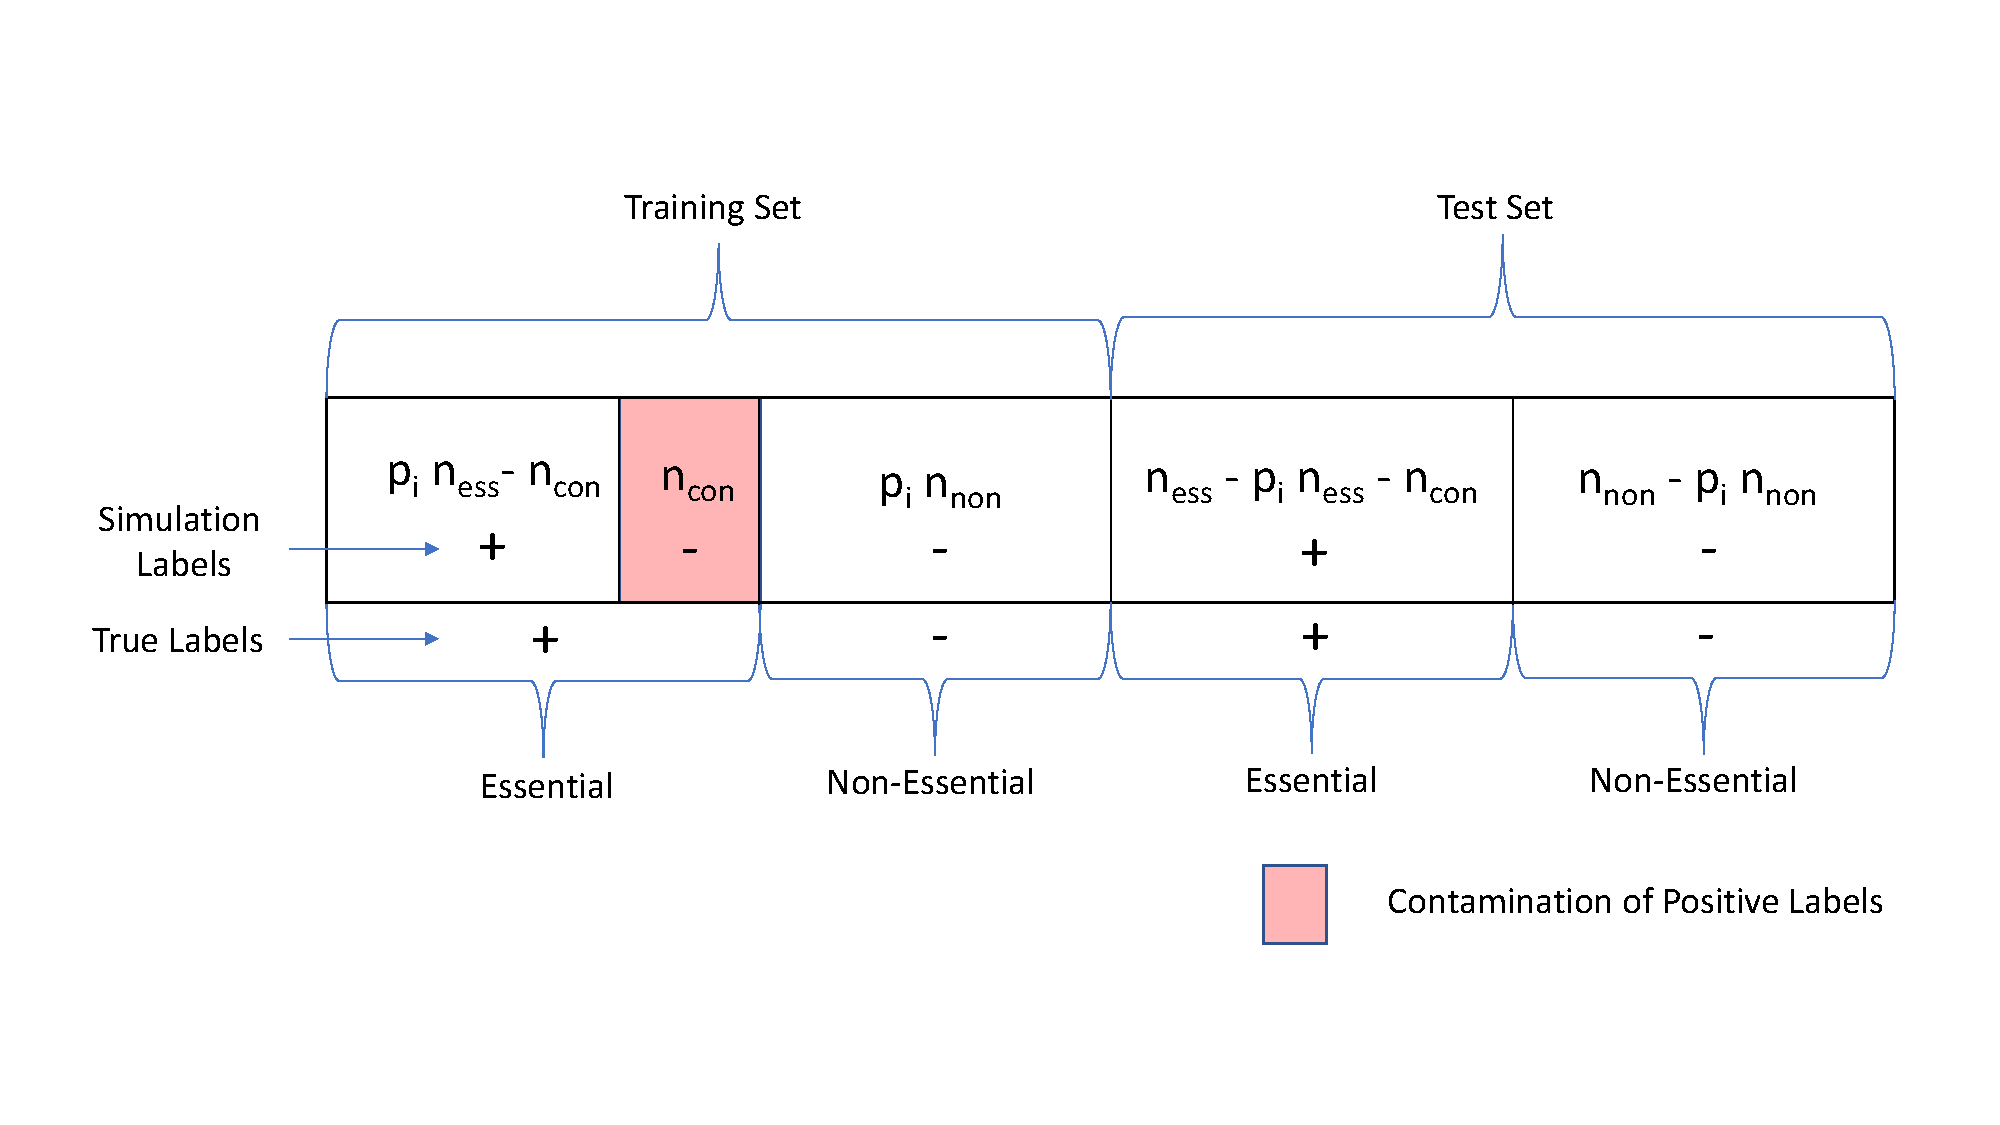
\includegraphics[width=0.9\textwidth]{unbalanced.pdf} 
    \vspace{1cm}
        \caption{\textbf{Diagram of unbalanced design describing true label contamination in training sets for supervised methods.} $p_{i}$, $n_{ess}$, $n_{con}$, and $n_{non}$ represent training set size, total number of essential genes, number of contaminated genes, total number of non-essential genes, respectively. $n_{con}$ is determined by contamination percentage of training set essential genes. Training and test sets are indicated above while true label of gene essentiality is indicted below figure. Simulation label describes the label assignment for analysis. Shaded area indicates the contamination of training set essential genes where simulation and true labels differ.} \label{fig:diagram}

\end{figure}

\begin{figure}
    \centering
%   \begin{subfigure}[t]{0.45\textwidth}
      \centering
%        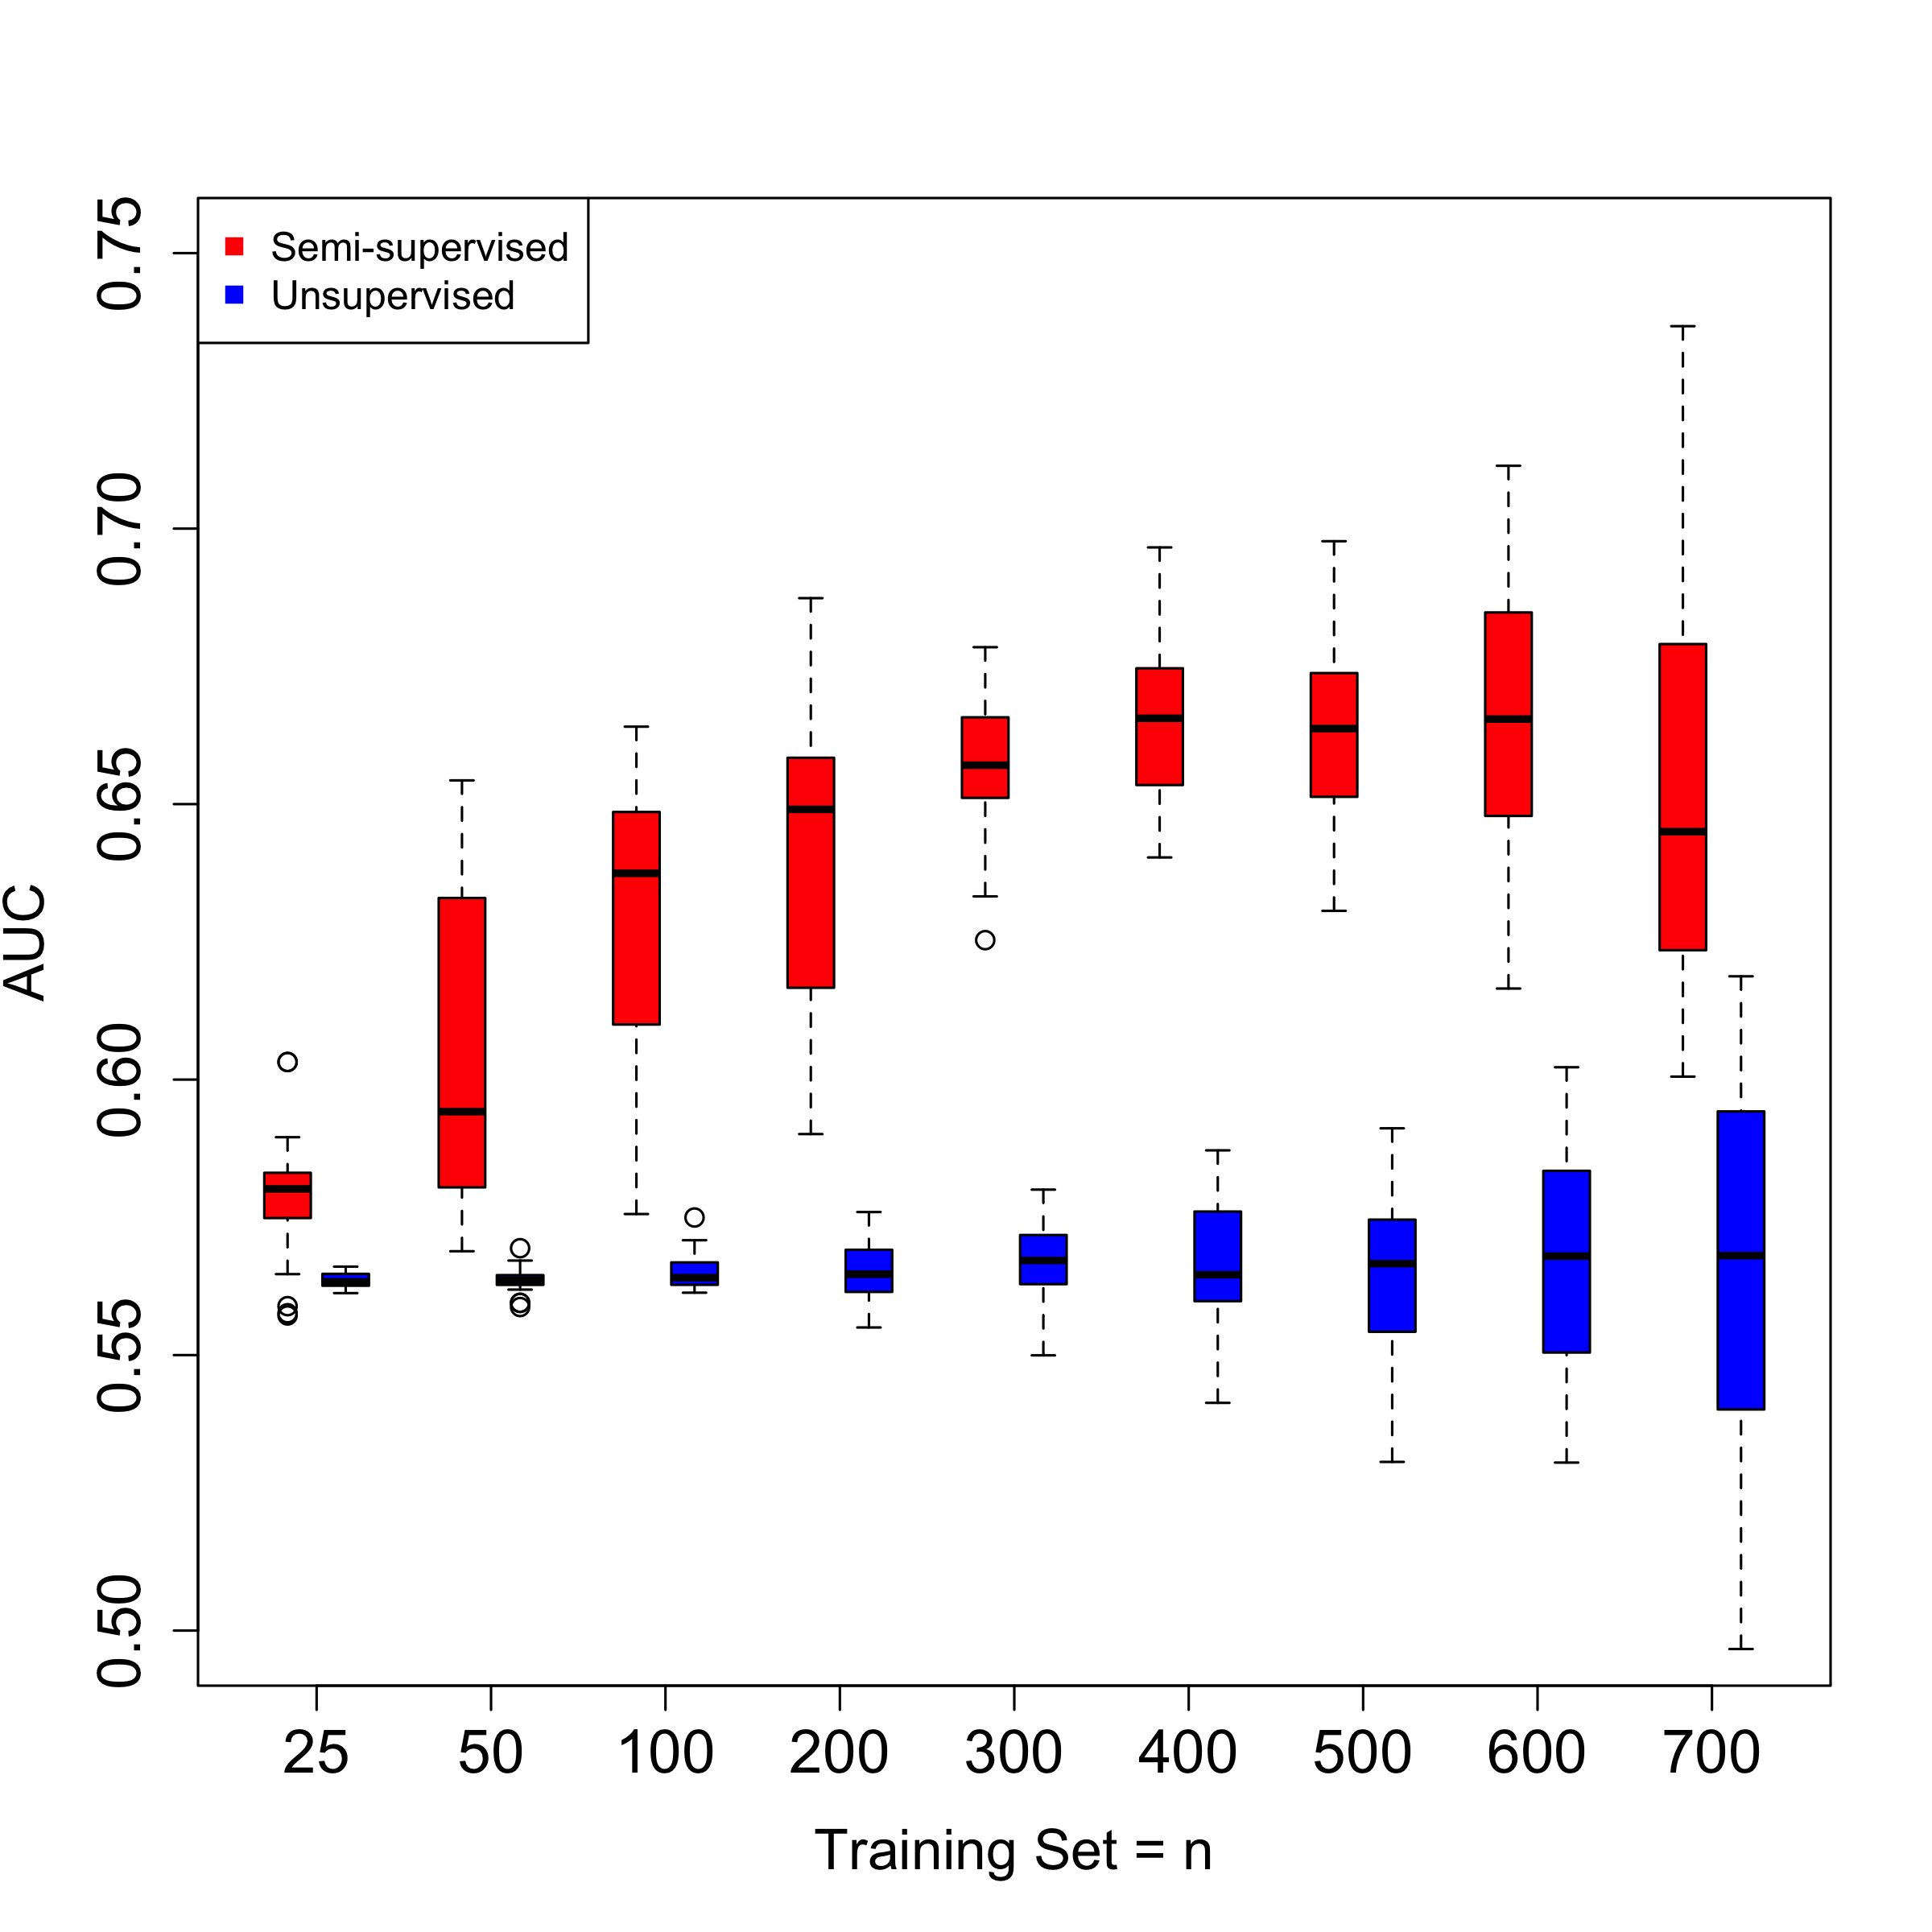
\includegraphics[width=1\linewidth]{6A-ROC_seqFeatures_pos_only_boxplots_post_post_2002_all_paper.png} 
        \caption{Sequence derived features.} \label{fig:unsup_seq}
%  \end{subfigure}
%    \begin{subfigure}[t]{0.45\textwidth}
        \centering
%        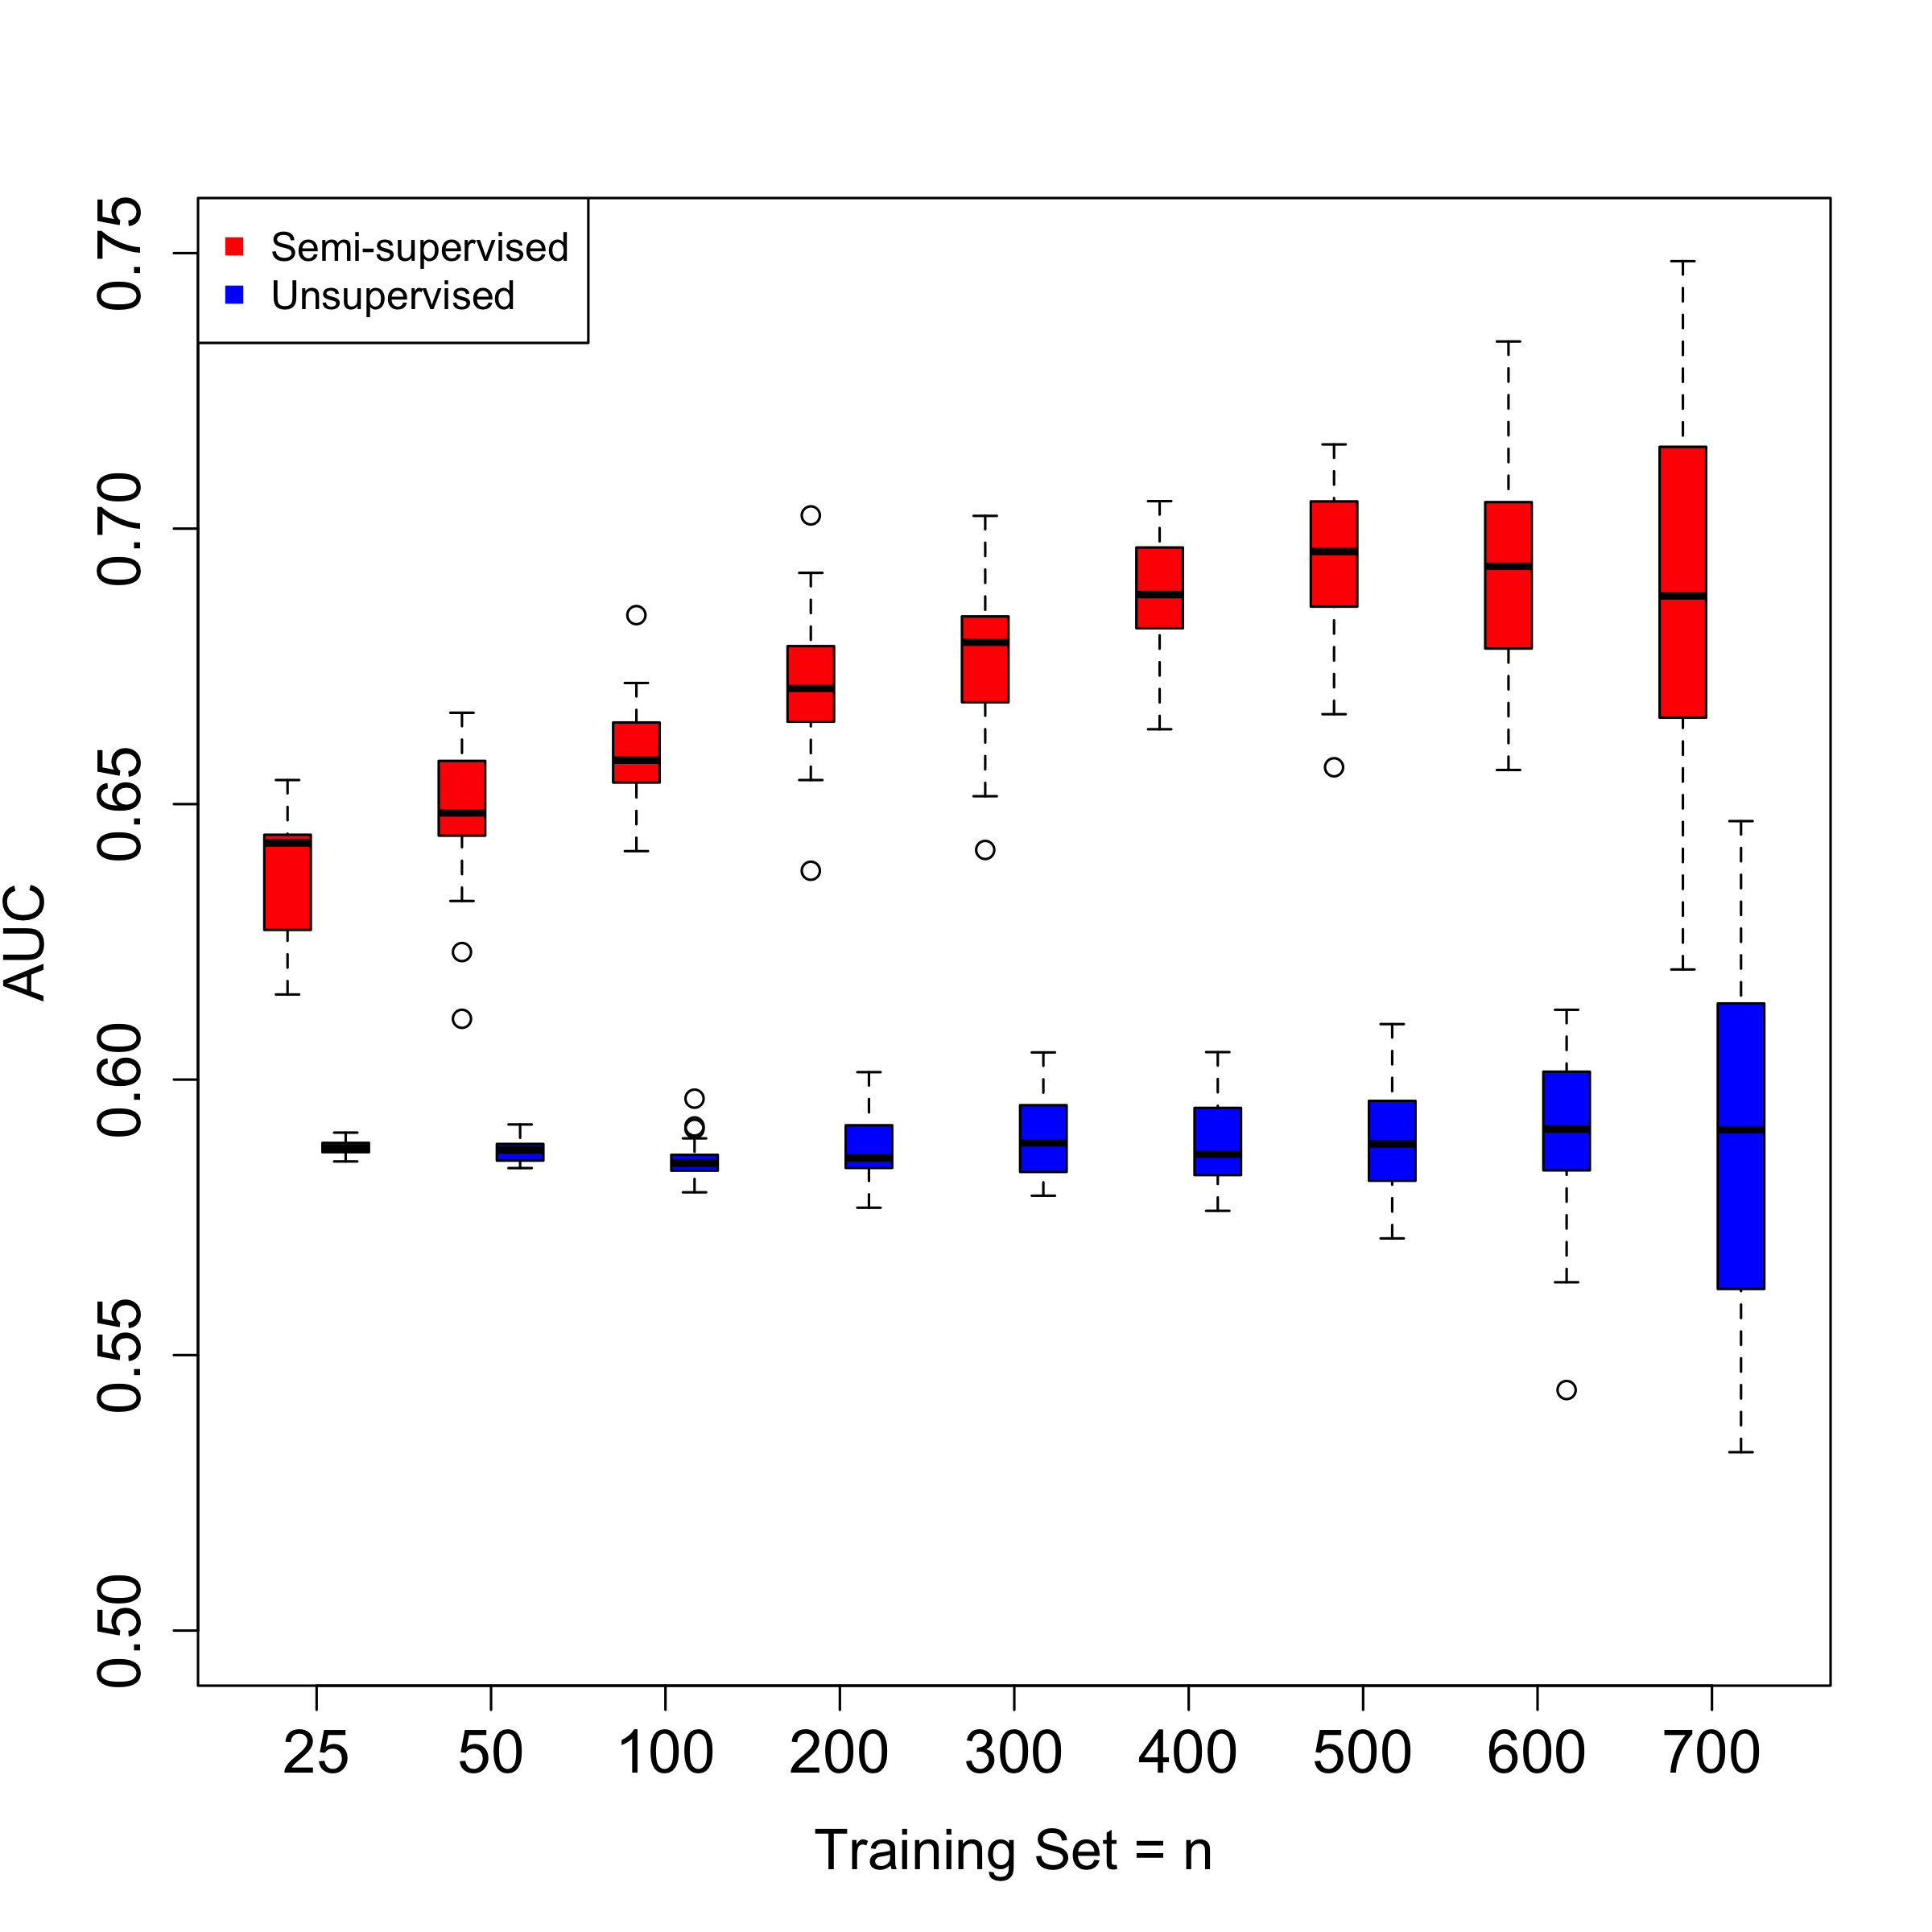
\includegraphics[width=1\linewidth]{6B-ROC_allFeatures_pos_only_boxplots_post_post_2002_all_paper.png} 
        \caption{All features.} \label{fig:unsup_all}
%    \end{subfigure}
    \vspace{1cm}
    \caption{\textbf{Boxplots of AUC at various training sizes of 769 essential genes using sequence derived (14) or all (22) features as predictors.} Semi-supervised and unsupervised method are shown in red and blue, respectively.}
    \label{fig:unsup}
\end{figure}


\begin{figure}[ht]
    \centering
%    \begin{subfigure}[b]{0.6\textwidth}
        \centering
%        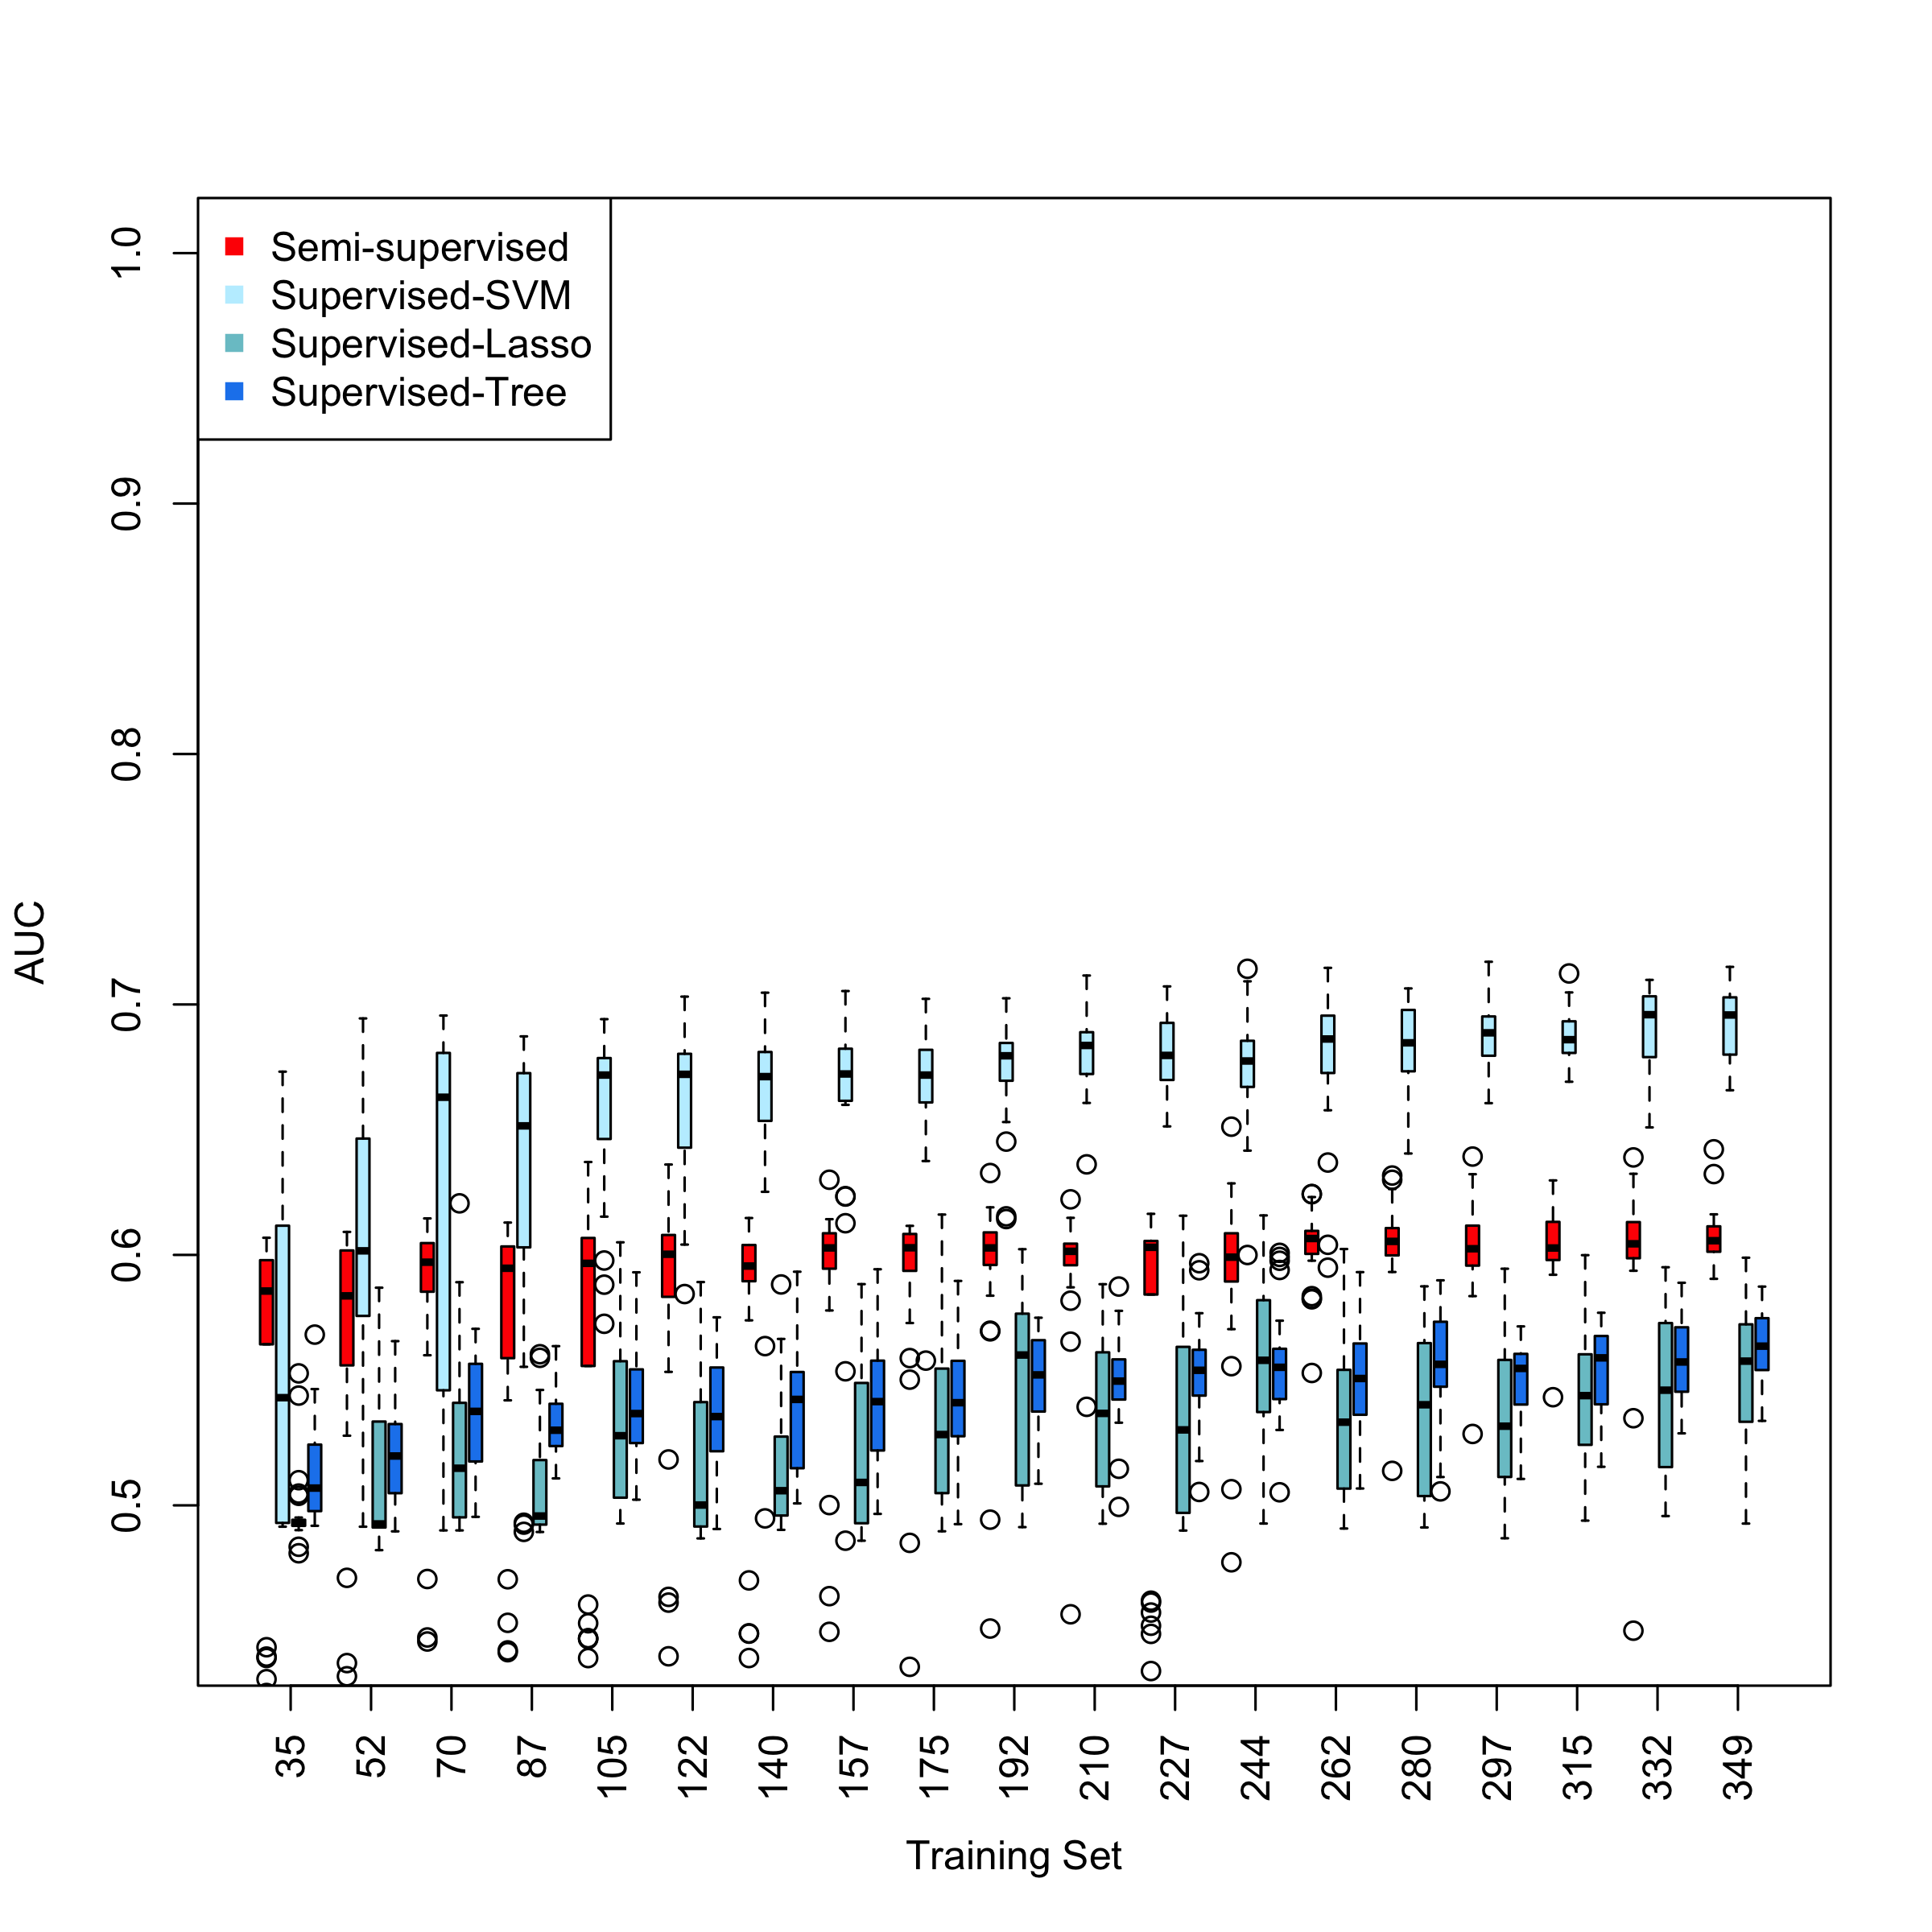
\includegraphics[width=\textwidth]{6D_allFeatures_unbalanced_0_paper.png} 
        \caption{0\% Contamination}
%    \end{subfigure}
    \centering
%   \begin{subfigure}[b]{0.45\textwidth}
        \centering
%        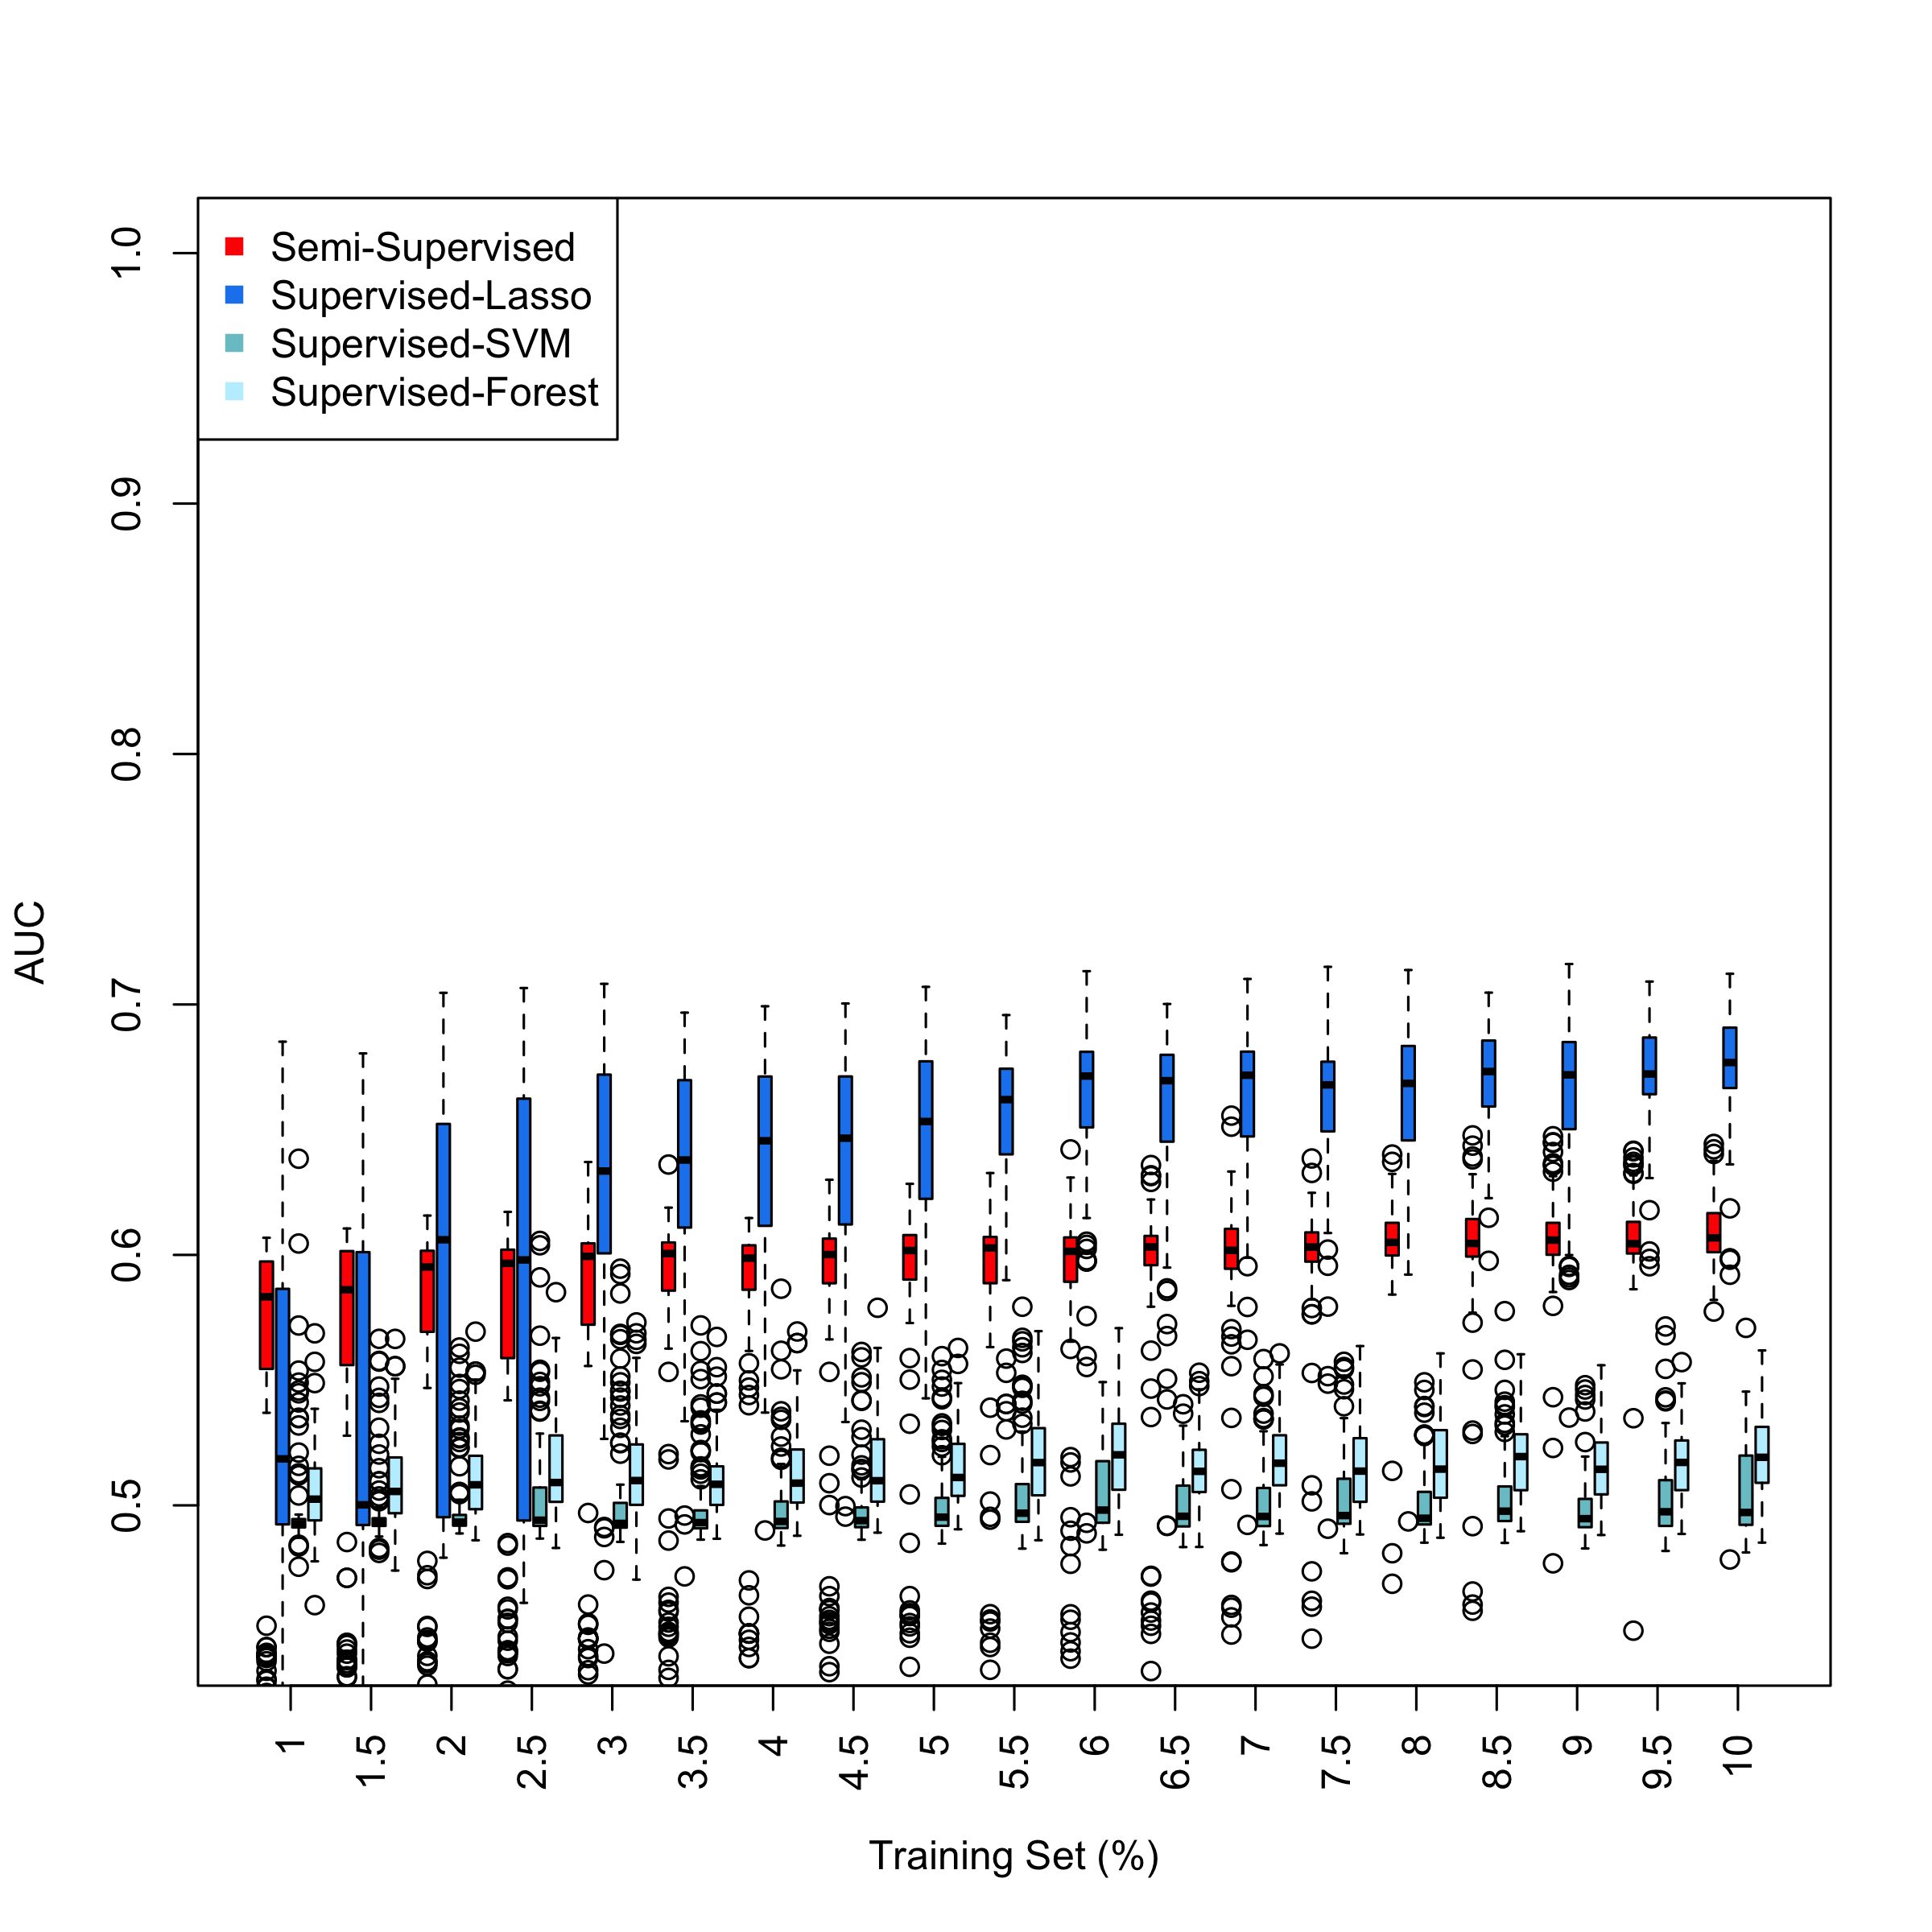
\includegraphics[width=0.8\textwidth]{6D_allFeatures_unbalanced_20_paper.png}
        \caption{20\% Contamination}
%    \end{subfigure}
    \centering
%    \begin{subfigure}[b]{0.45\textwidth}
        \centering
 %       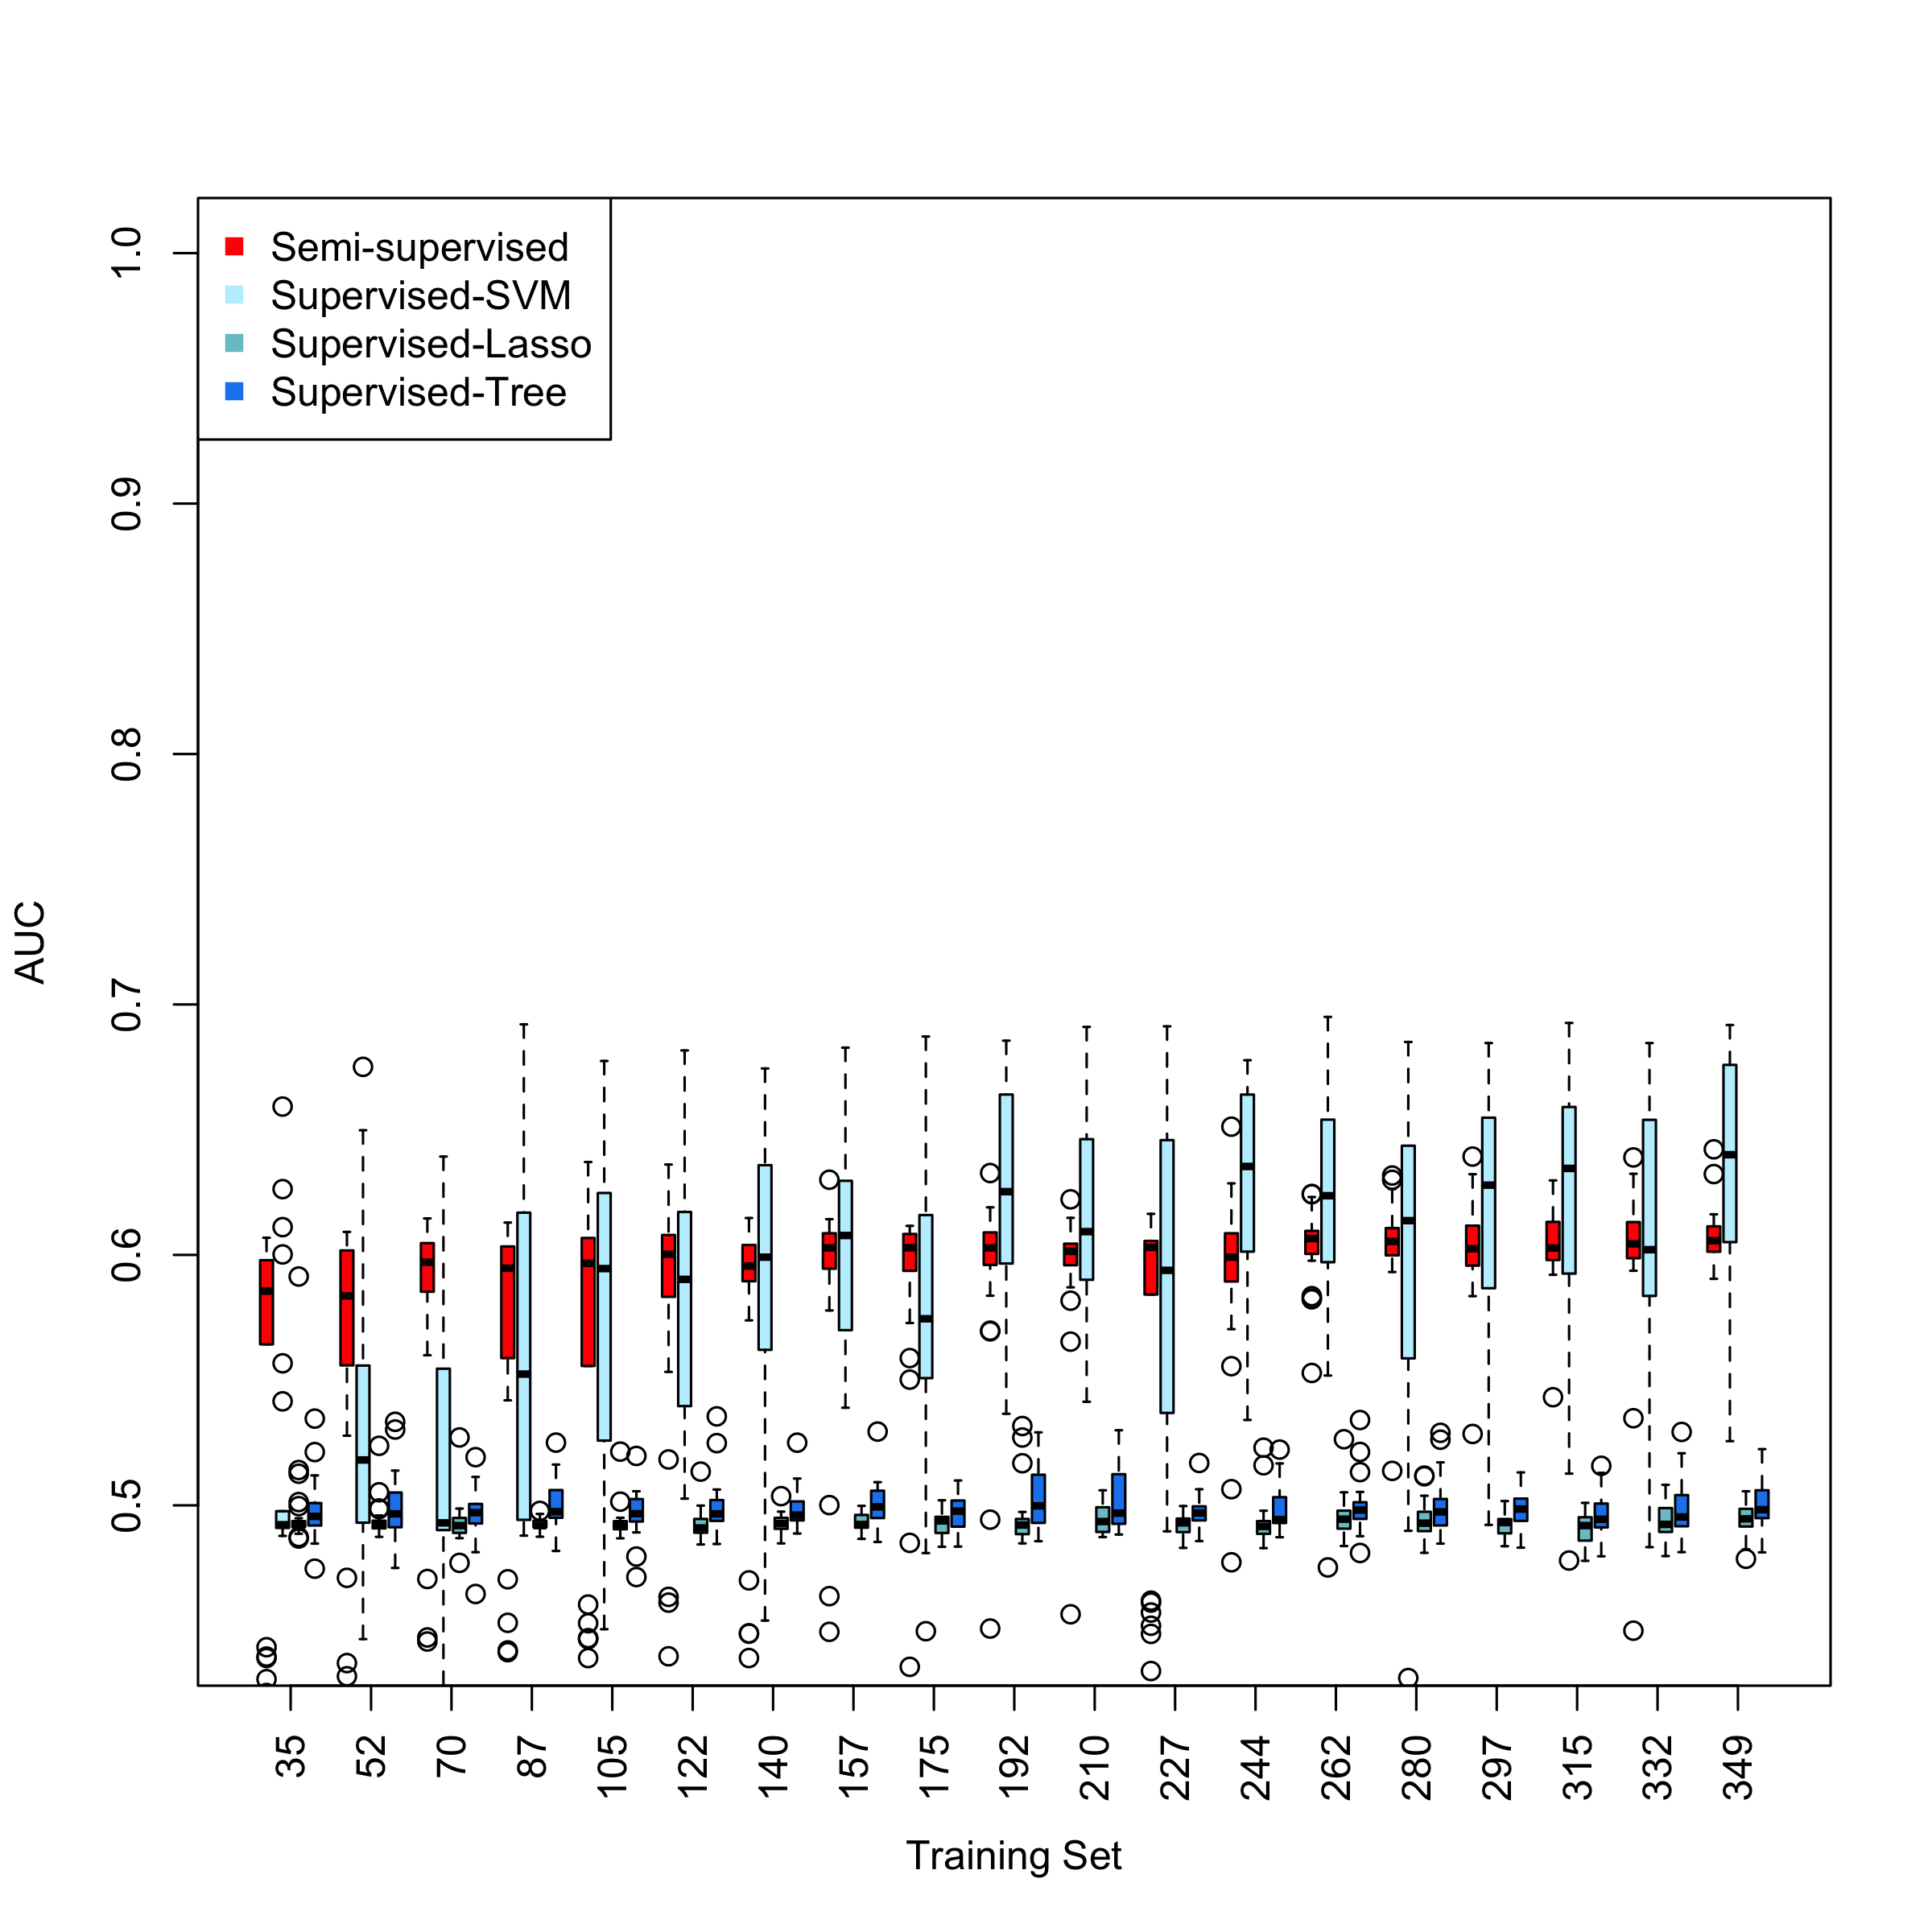
\includegraphics[width=0.8\textwidth]{6D_allFeatures_unbalanced_50_paper.png}
        \caption{50\% Contamination}
%    \end{subfigure}
    \vspace{1cm}
    \caption{\textbf{AUC comparison between semi-supervised and supervised methods at various training sizes with all essential genes in yeast using 19 features as predictors.} 100 iterations were executed at training sets percentages  (1, 1.5, 2, ... ,10) for all four methods and negative contamination levels (0\% (a), 20\% (b), and 50\% (c)). Semi-supervised method is shown in red while the supervised methods (LASSO, SVM, and Random Forest) are shown in blue, aquamarine, and light blue, respectively.}
    \label{fig:AUCboxplots}
\end{figure}

\begin{figure}[ht]
    \centering
%    \begin{subfigure}[b]{0.6\textwidth}
%      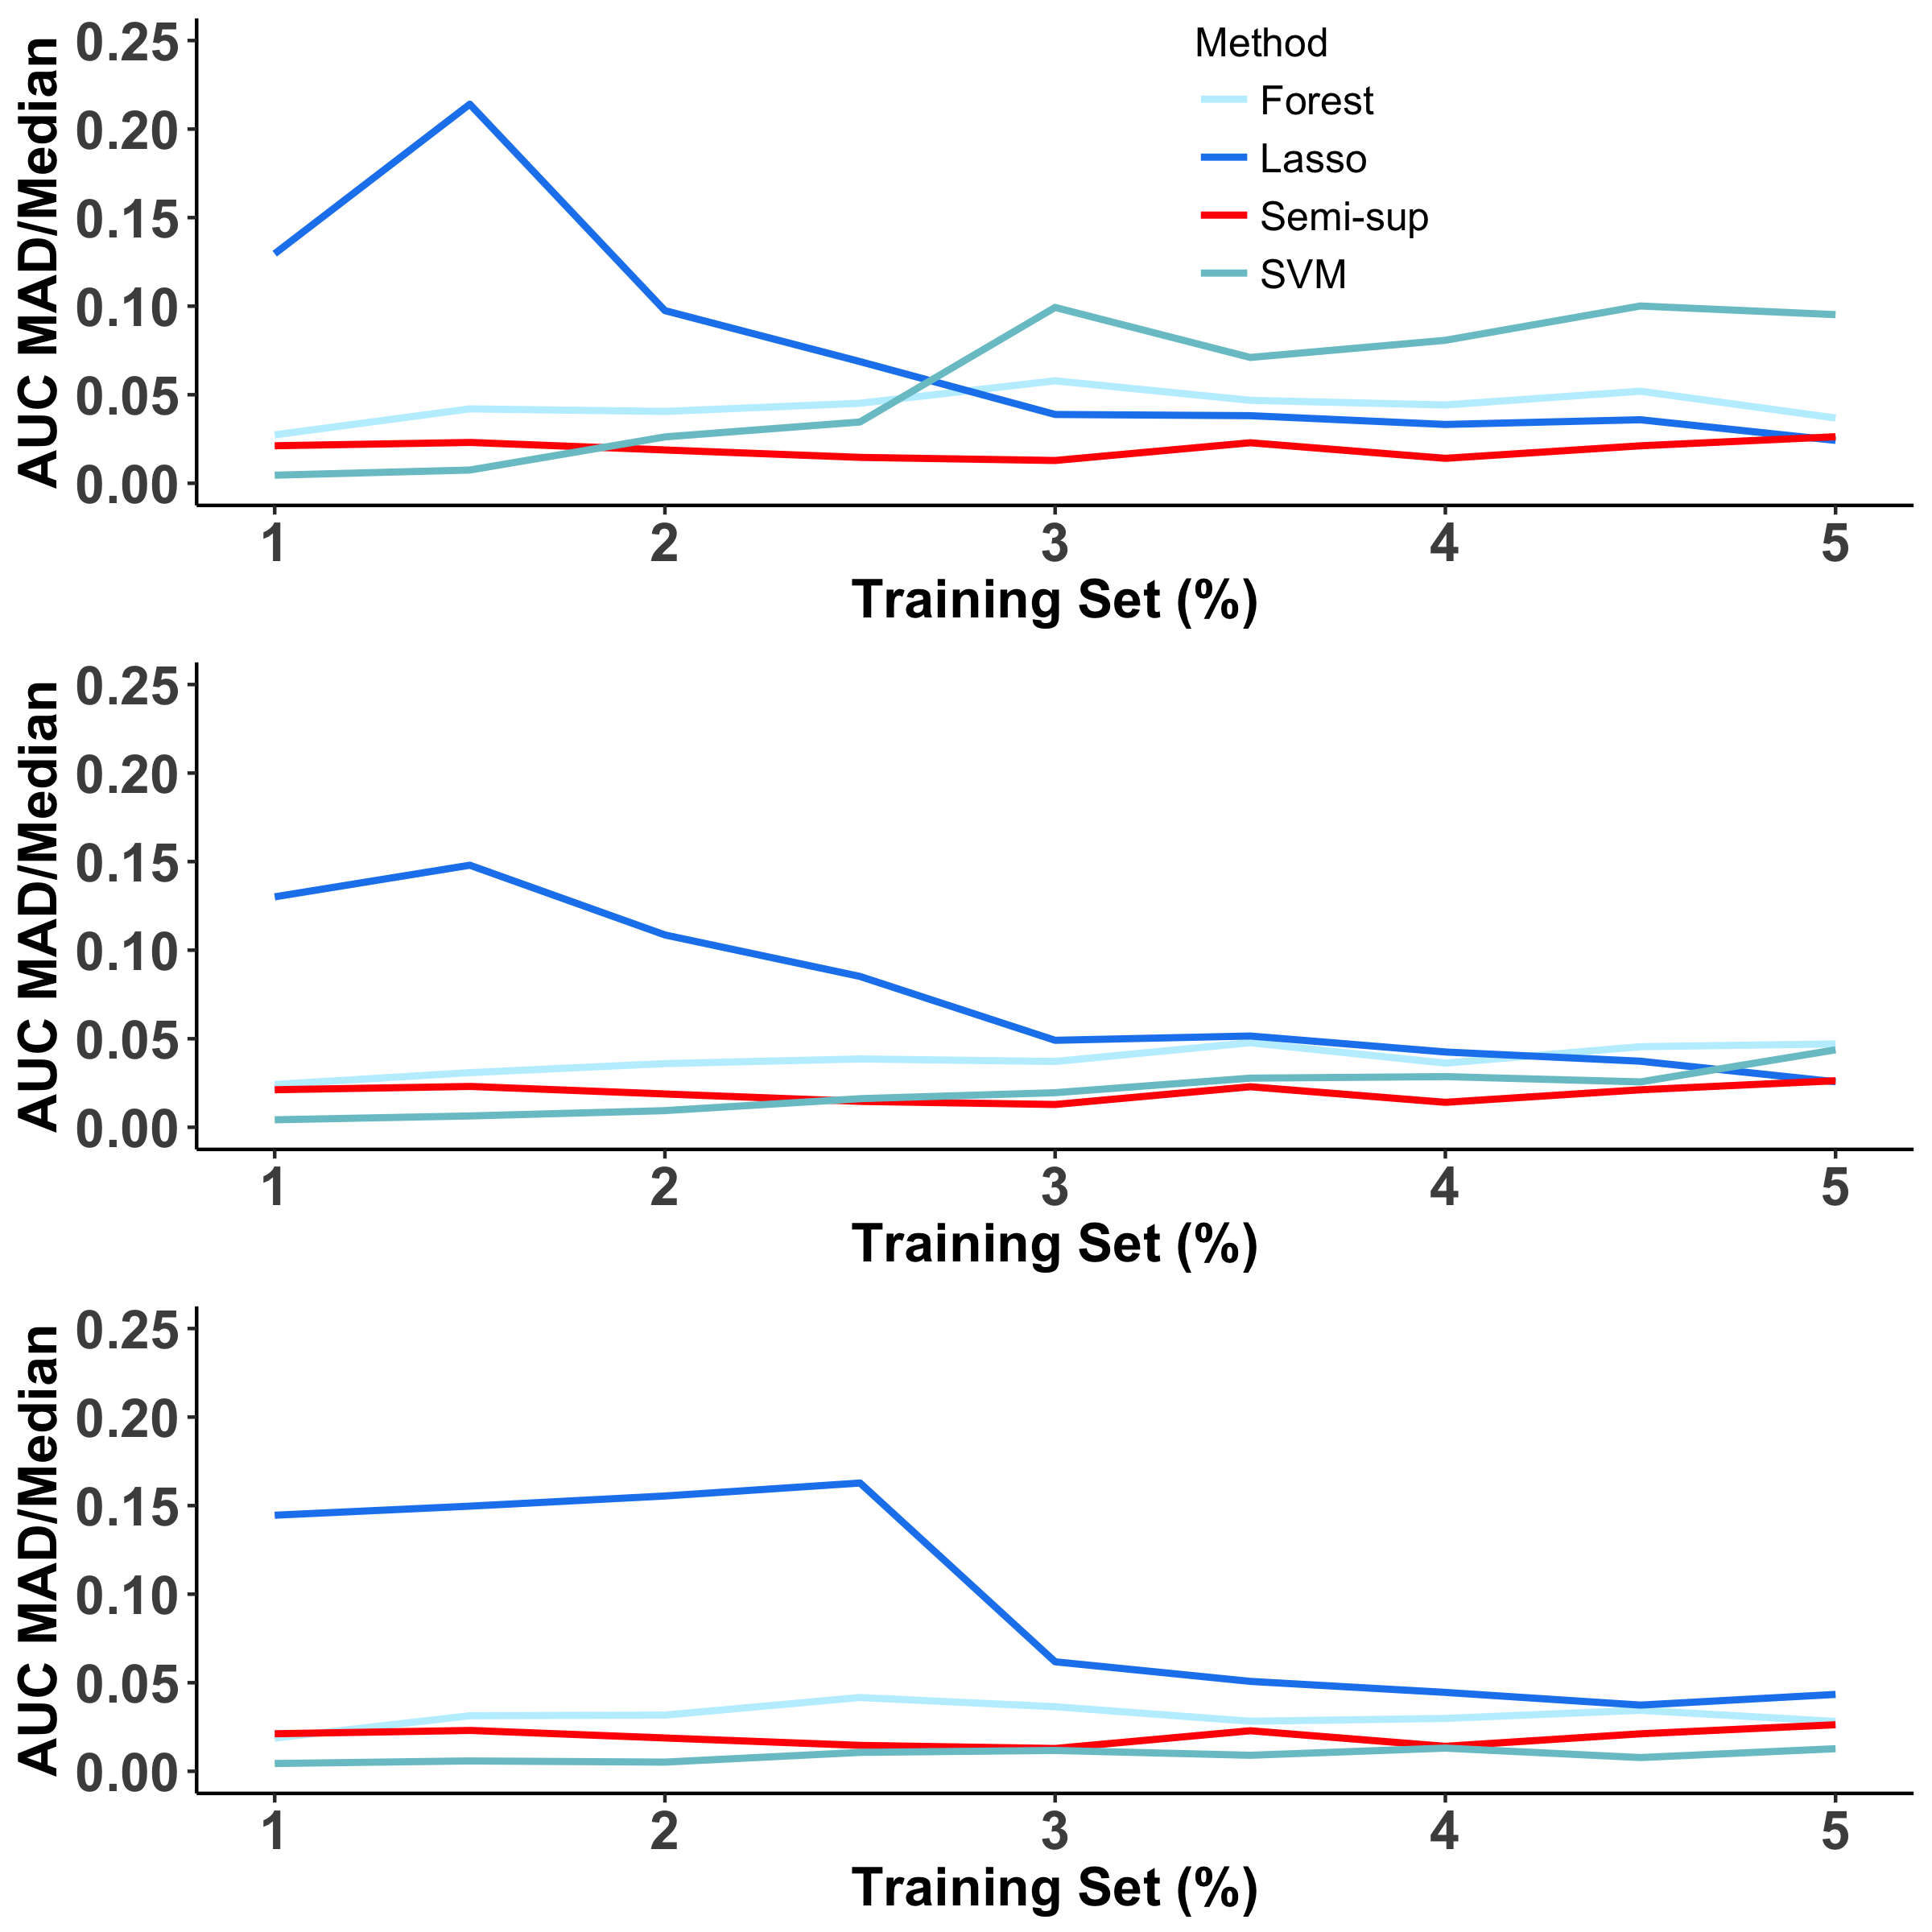
\includegraphics[width=\textwidth]{AUCcvmed.png}
        \caption{AUC MAD/Median}
 %   \end{subfigure}
  %  \begin{subfigure}[b]{0.45\textwidth}
%     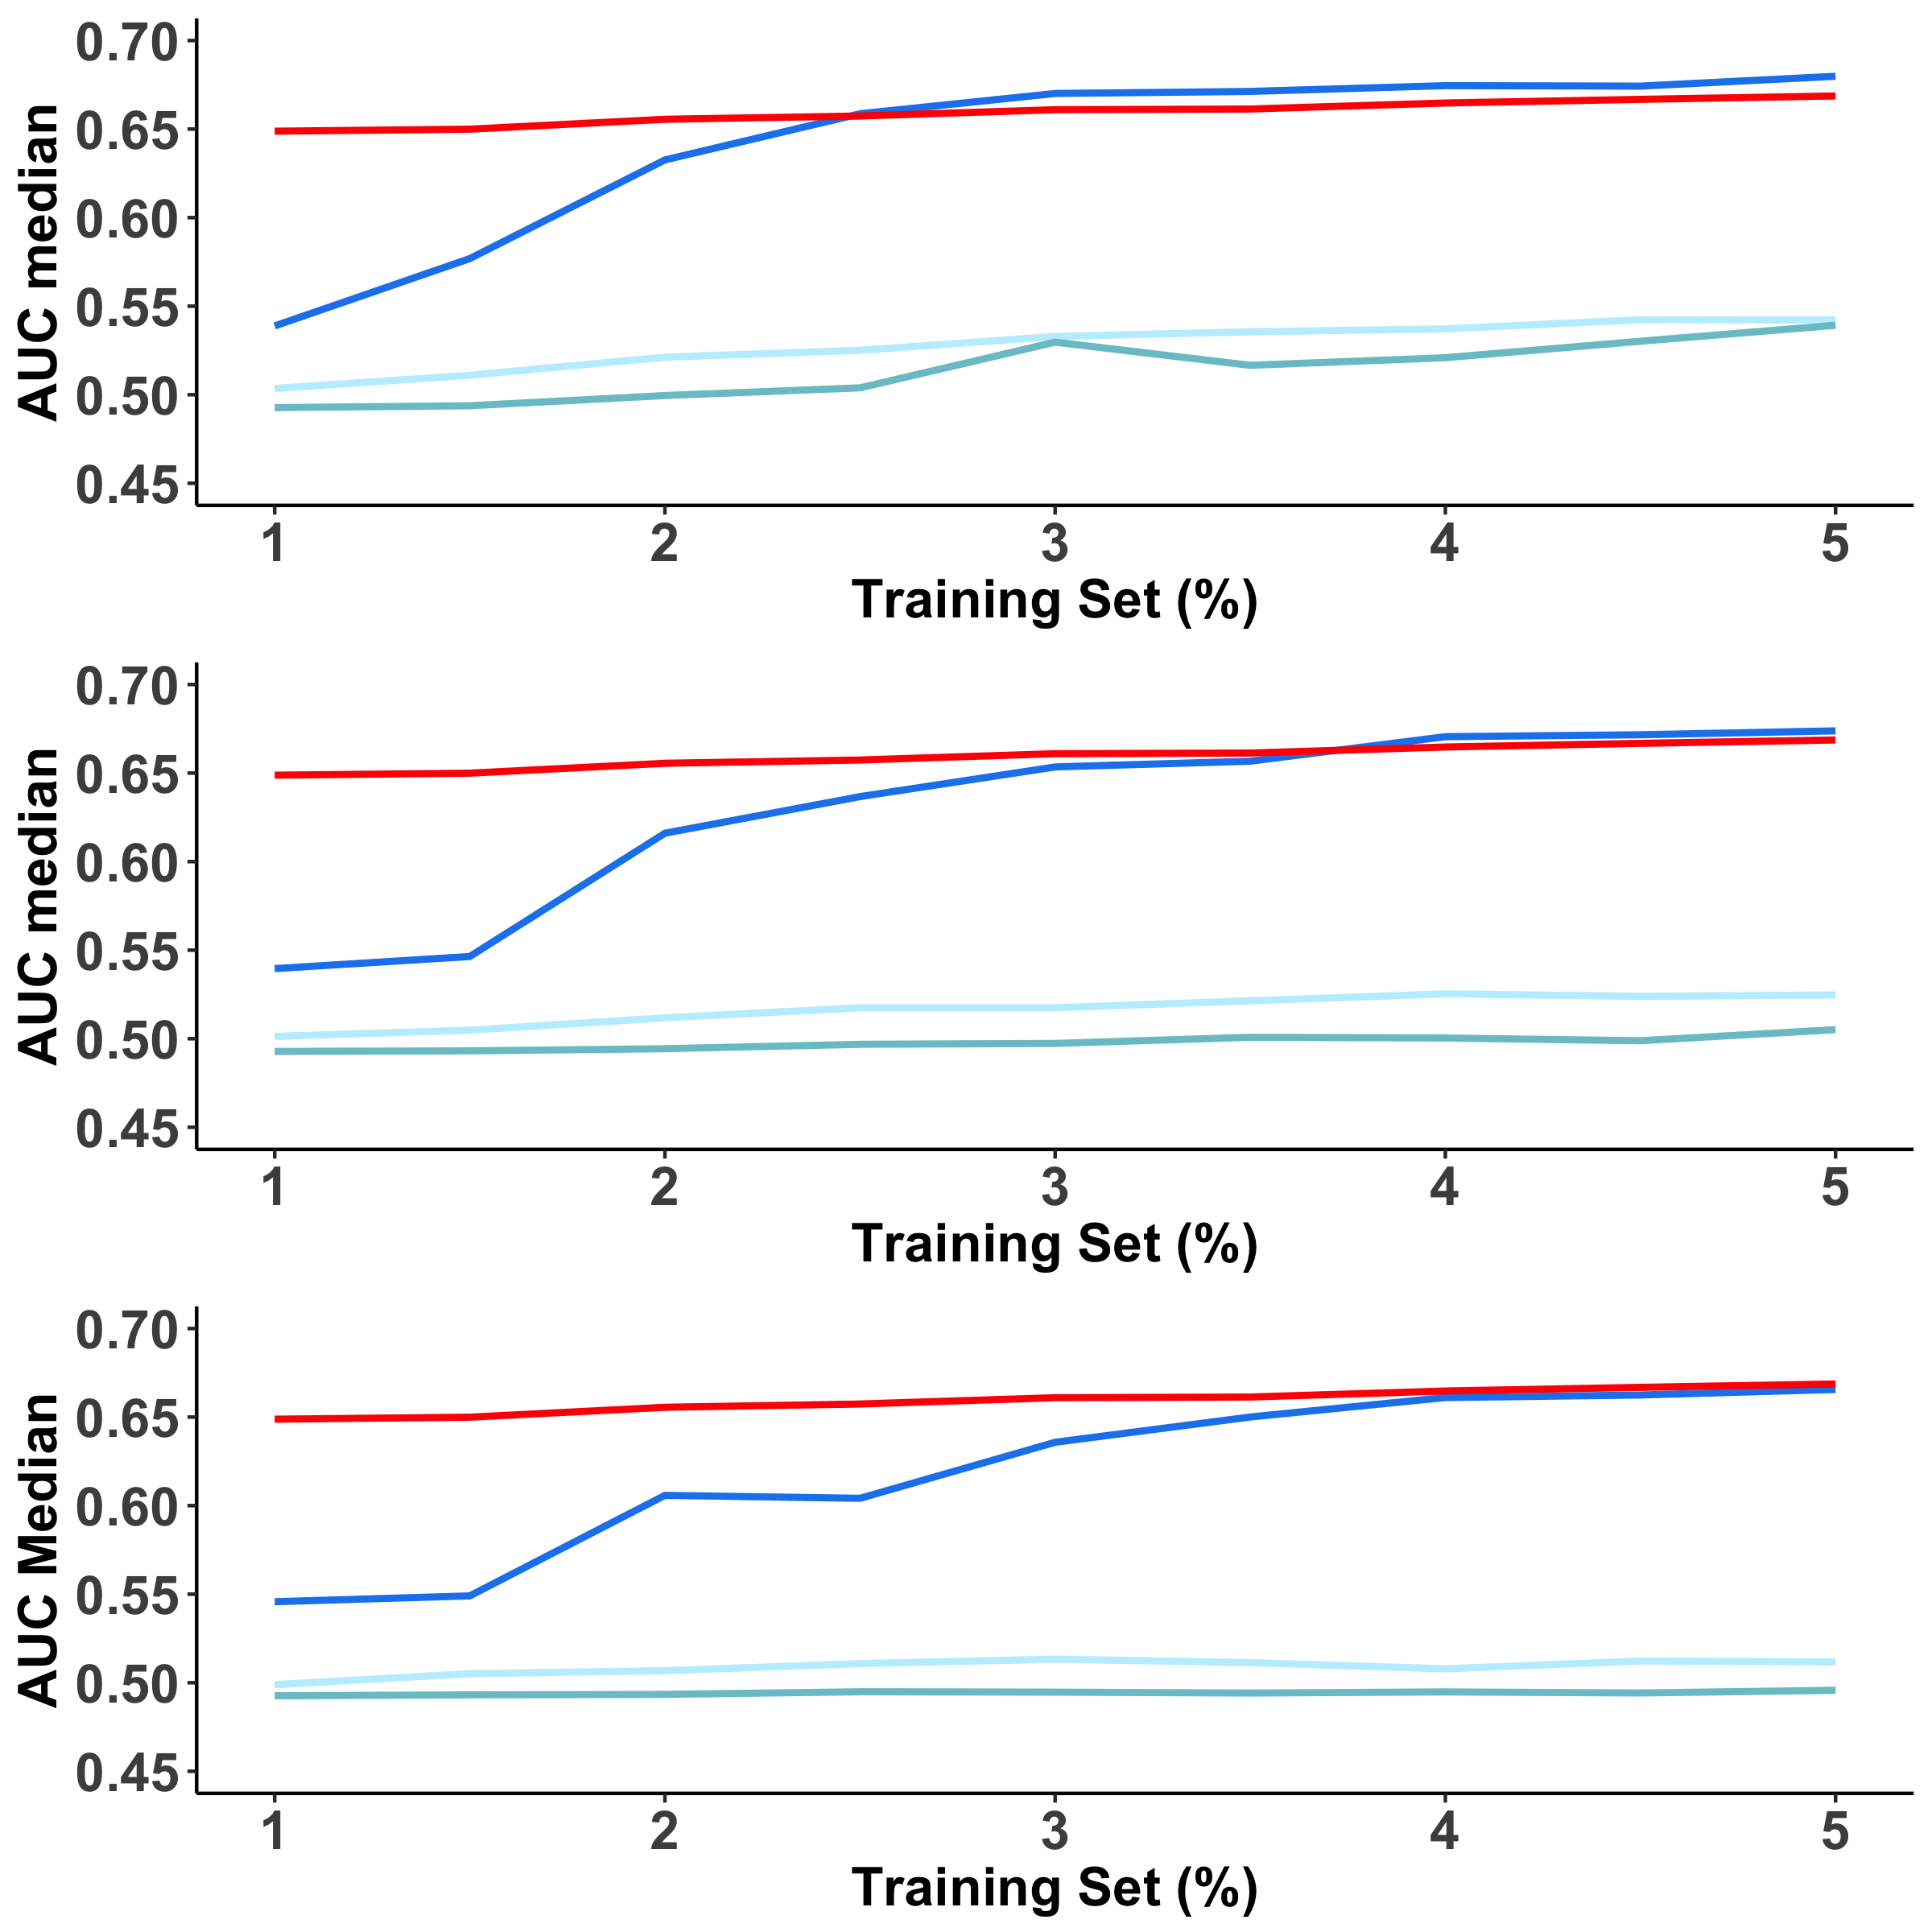
\includegraphics[width=\textwidth]{AUCmed.png} 
        \caption{AUC Median}
%    \end{subfigure}
%    \begin{subfigure}[b]{0.45\textwidth}
%        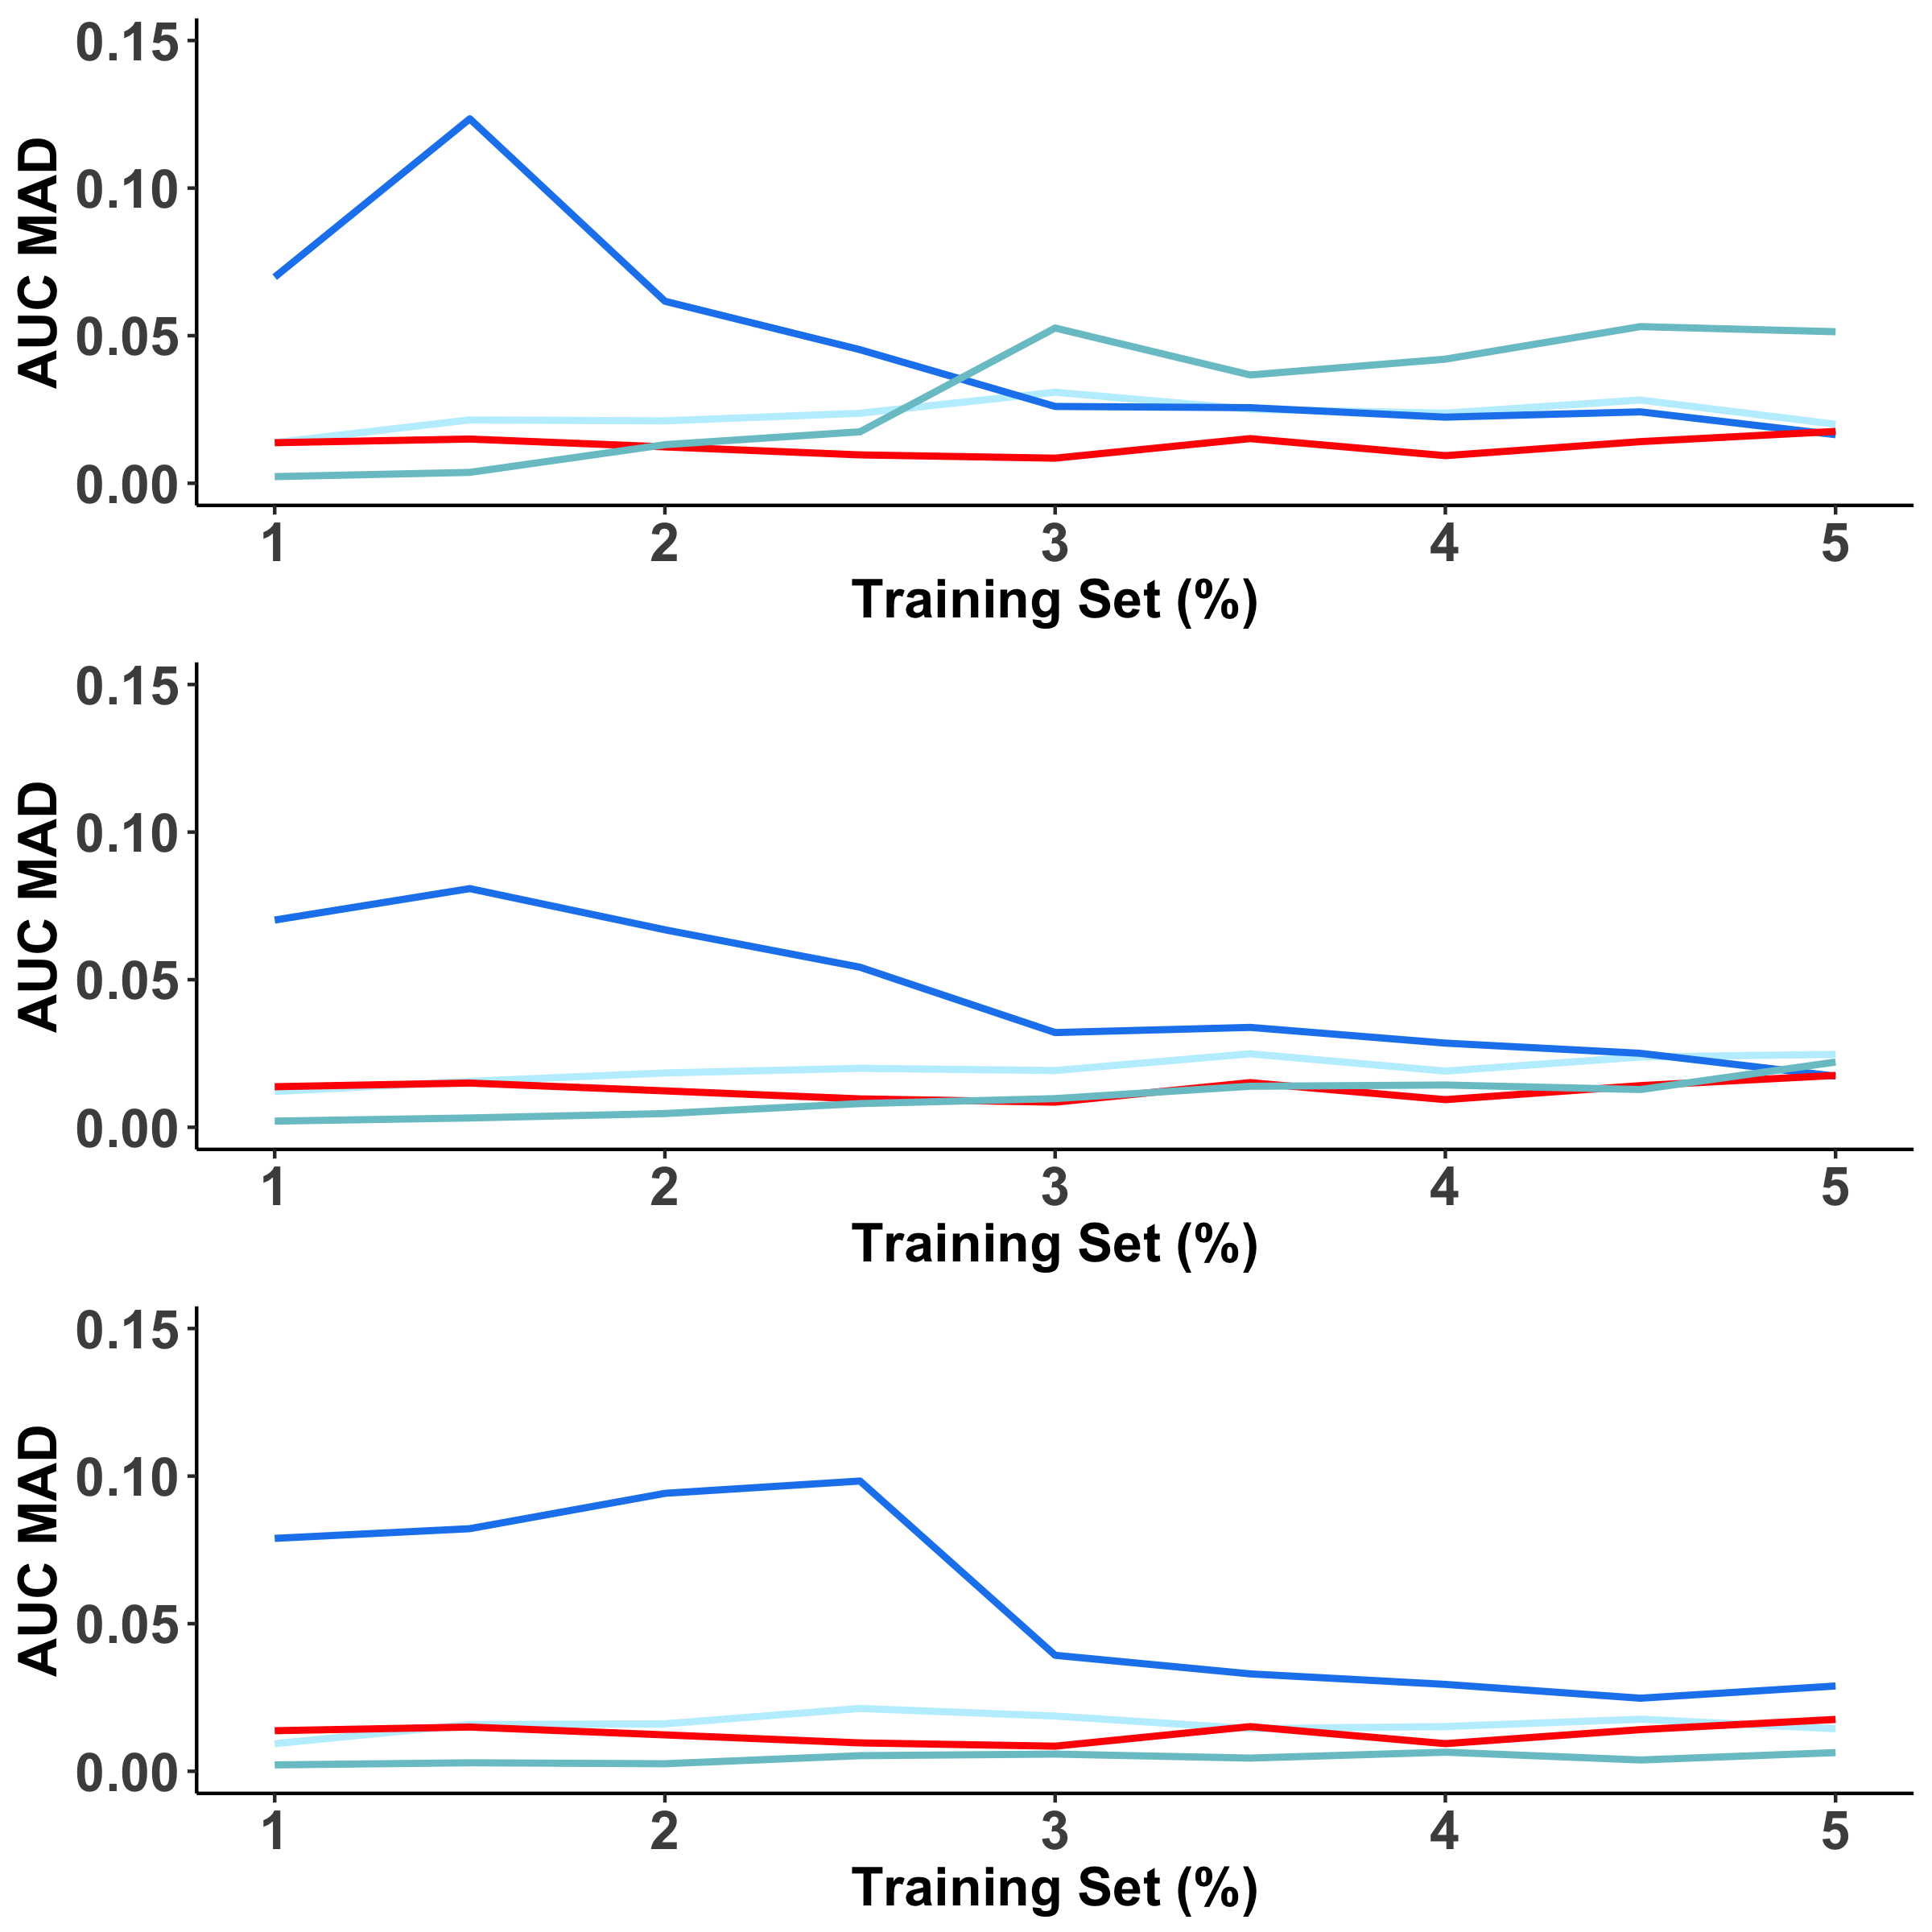
\includegraphics[width=\textwidth]{AUCmad.png} 
        \caption{AUC Median Absolute Deviation}
%    \end{subfigure}
    \vspace{1cm}
    \caption{\textbf{Evaluation of summary statistics comparing semi-supervised and supervised methods.} 100 iterations were executed at training sets (1\%, 1.5\%, 2\%,...,5\%) for all four methods and negative contamination levels (0\%, 20\%, and 50\%). Semi-supervised method is shown in red while the supervised methods (LASSO, SVM, and Random Forest) are shown in blue, aquamarine, and light blue, respectively. The AUC mean (a), variance (b), and CV (c) contrasts the four methods at each training set size across three contamination rates. CV is calculated as the Median Absolute Deviation (MAD)/Median}
    \label{fig:AUCsummarymedian}
\end{figure}

\begin{figure}[ht]
    \centering
%    \begin{subfigure}[b]{0.45\textwidth}
%        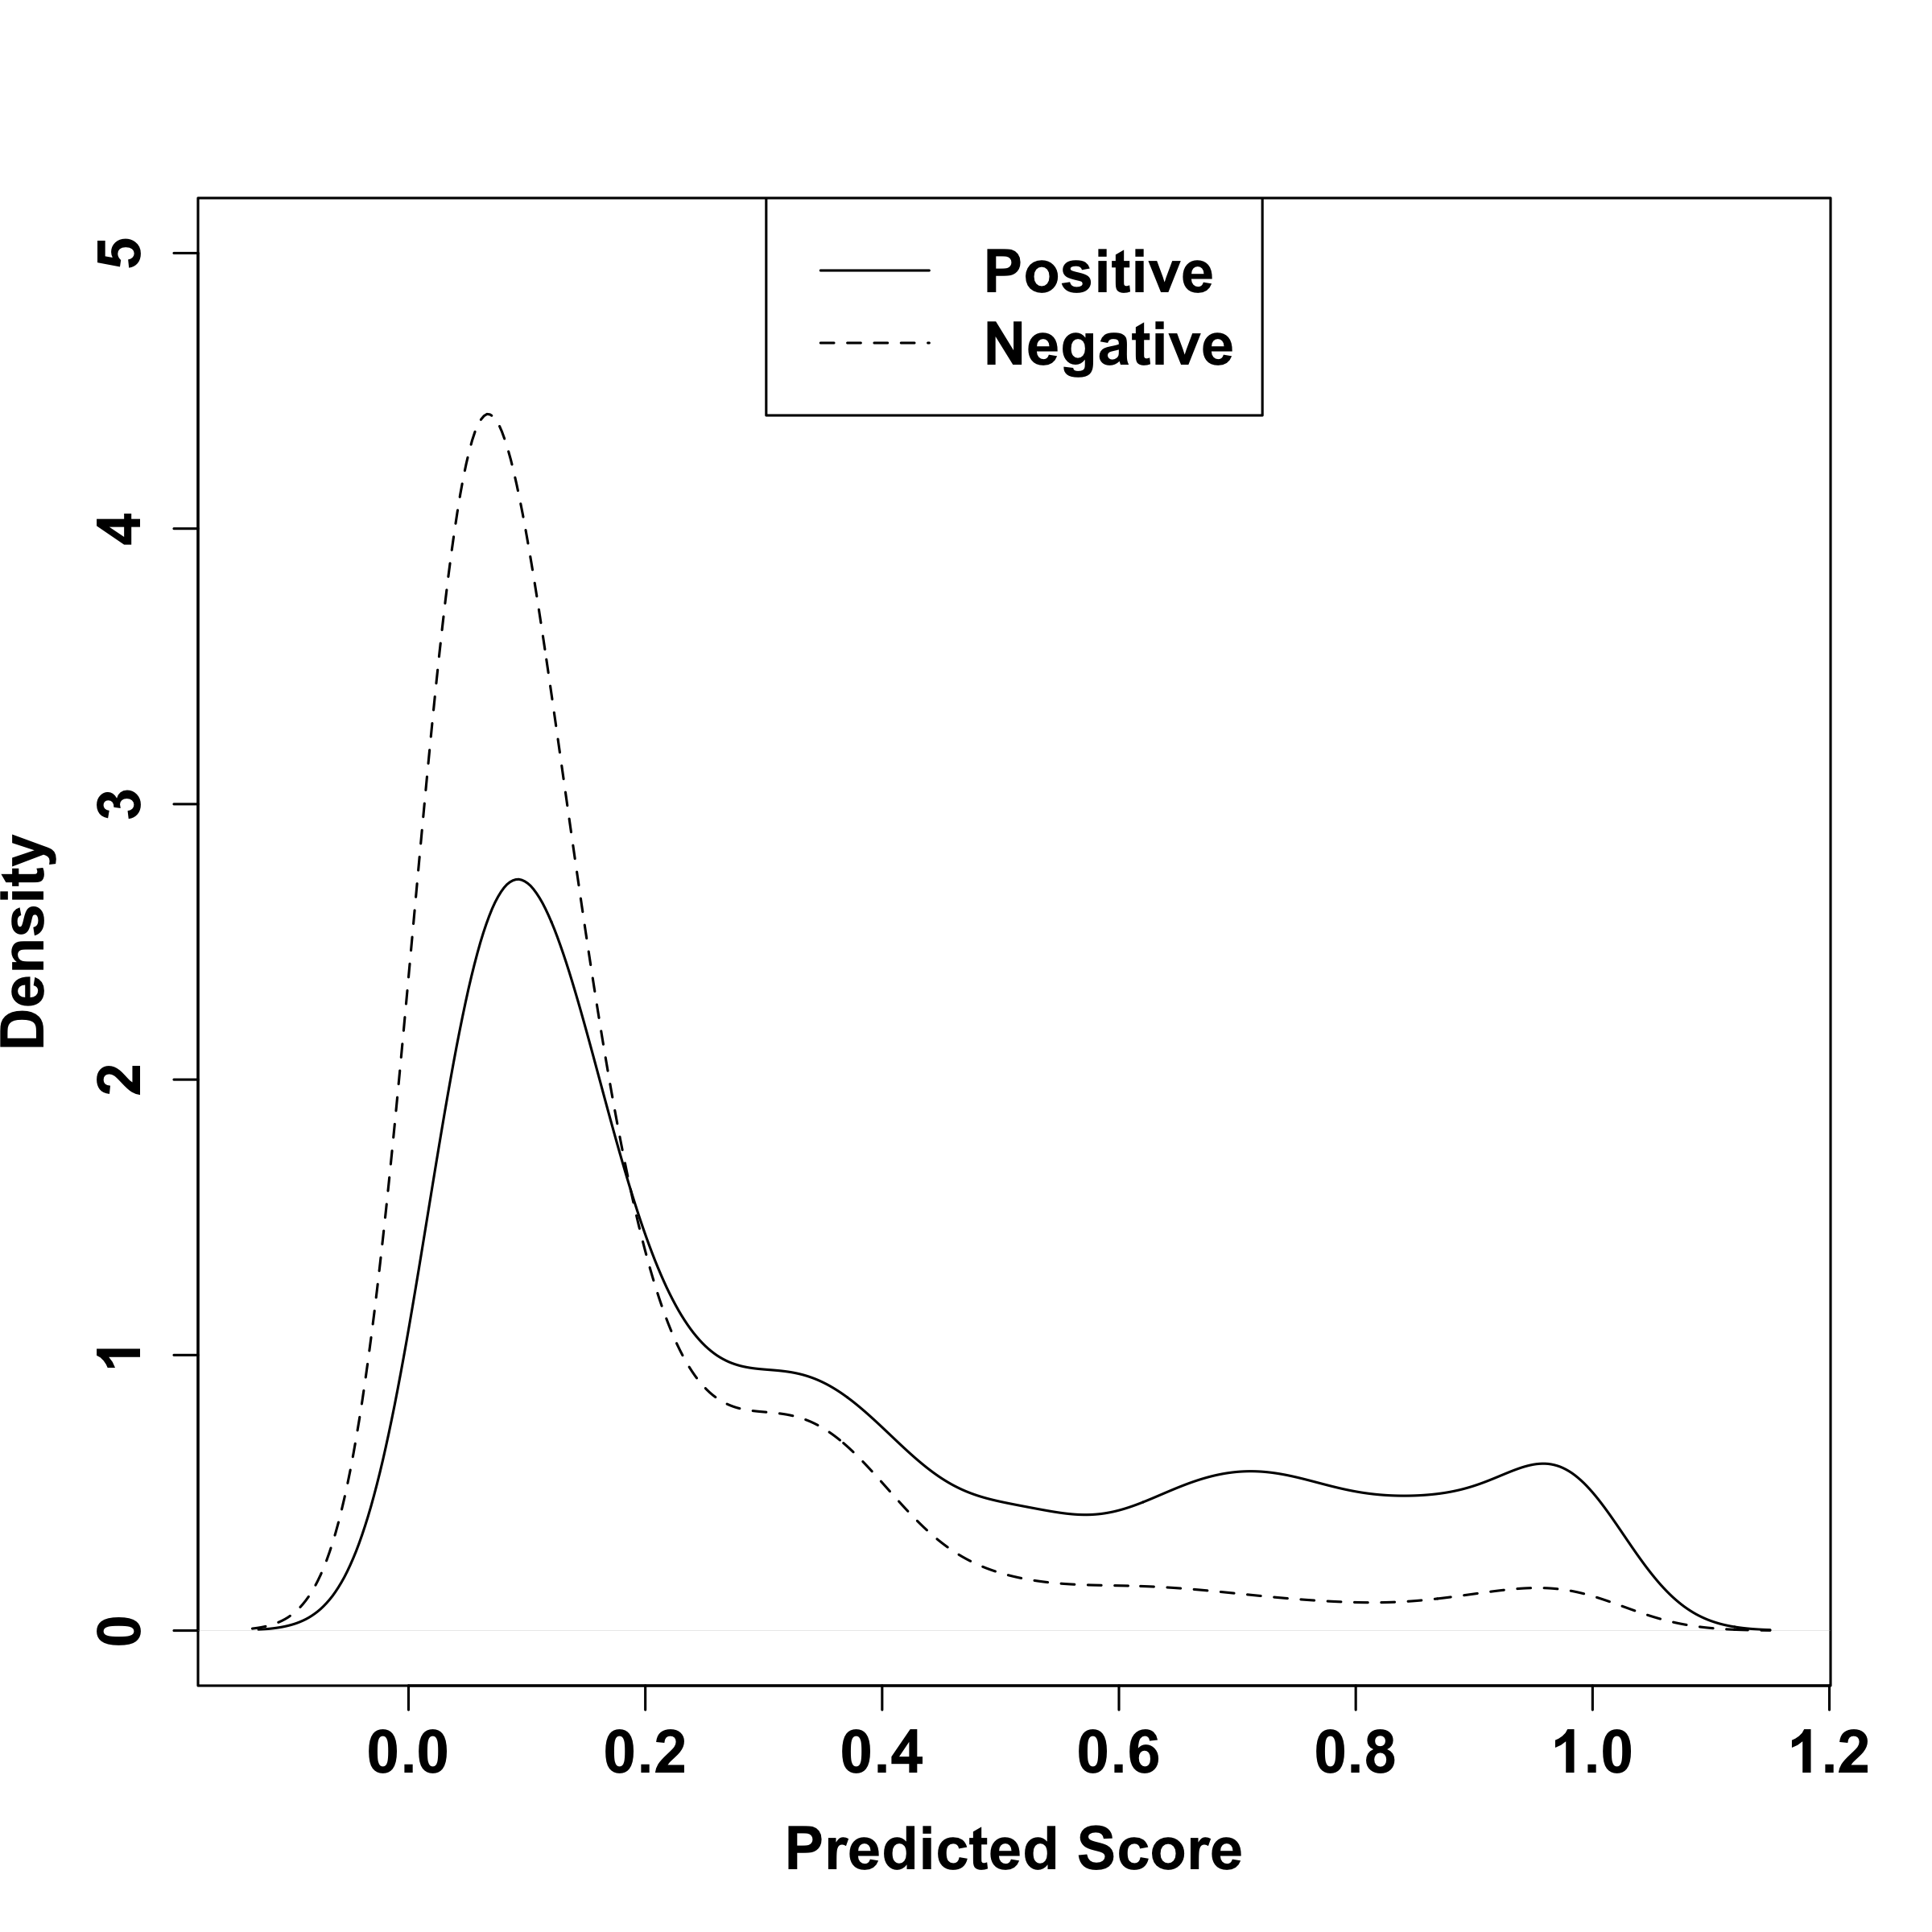
\includegraphics[width=\textwidth]{Lasso_Histogram_1_Training_0_Contamination.png}
        \caption{LASSO}
%    \end{subfigure}
%    \begin{subfigure}[b]{0.45\textwidth}
%        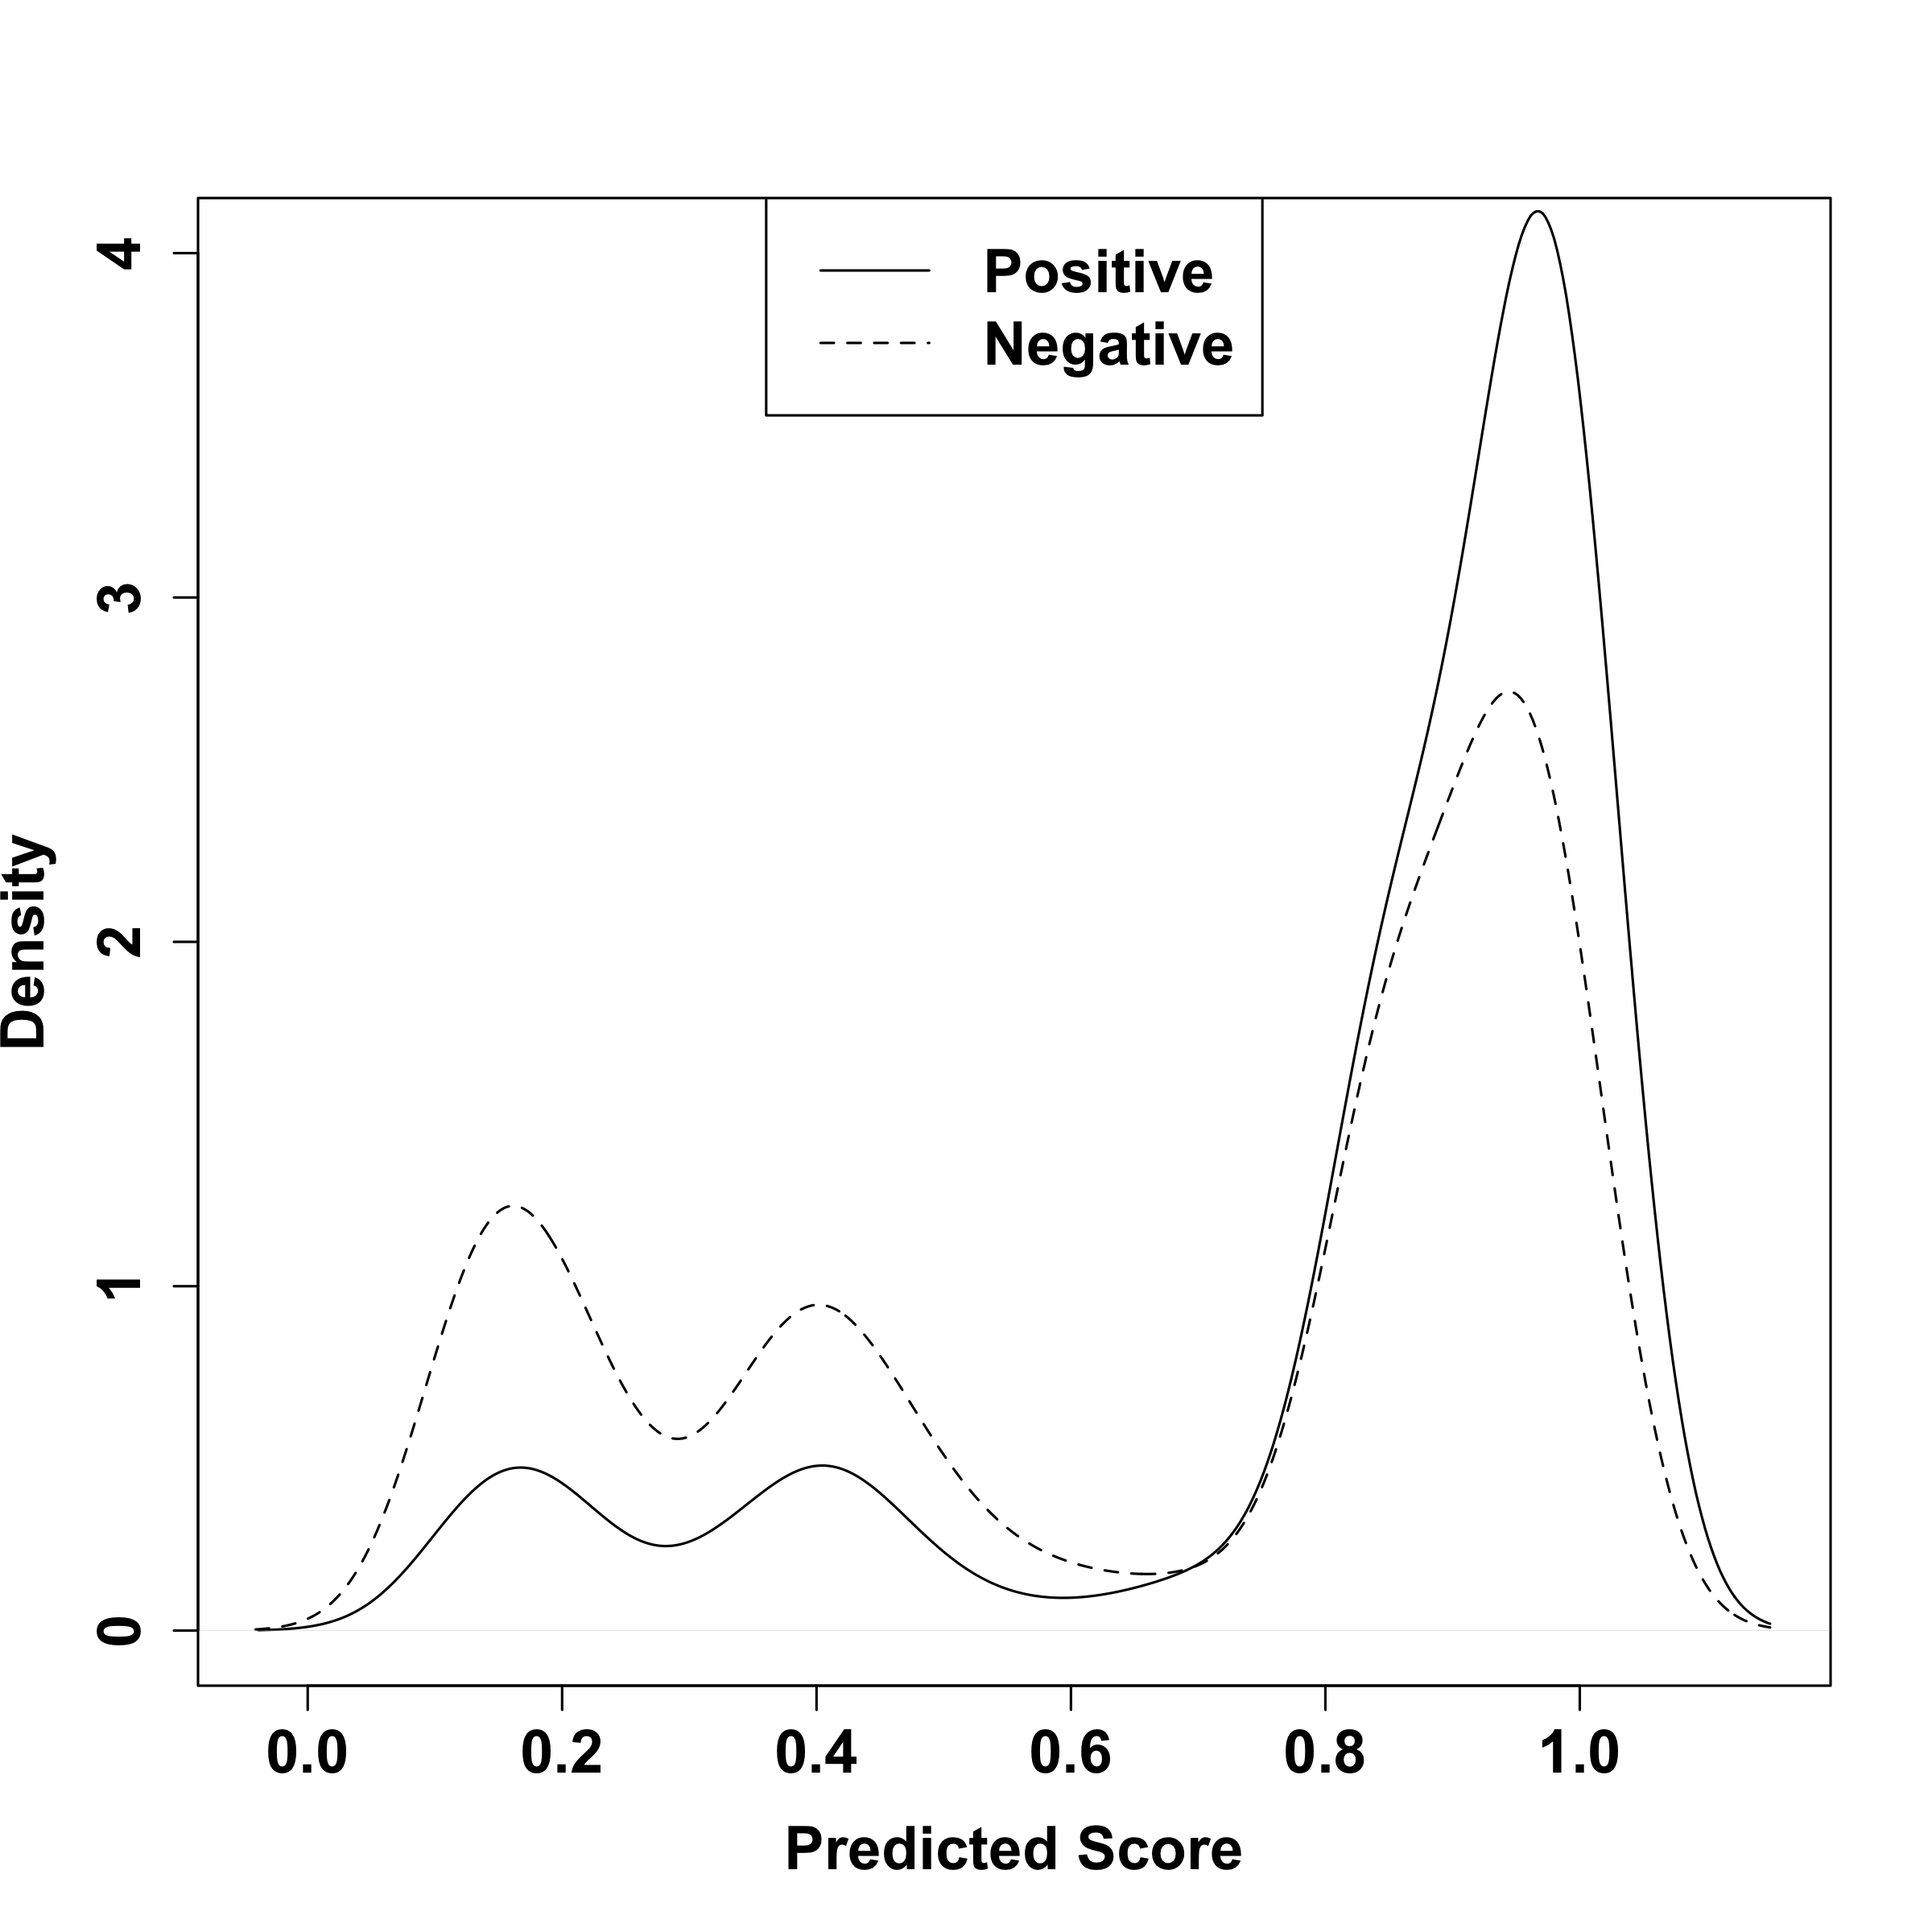
\includegraphics[width=\textwidth]{Semi_Histogram_1_Training_0_Contamination.png}
        \caption{Semi-Supervised}
%    \end{subfigure}
\vspace{1cm}
    \caption{\textbf{Density plot of predicted scores juxtaposing semi-supervised and LASSO methods.} LASSO (a) and Semi-Supervised (b) methods display kernel densities for true positive (dashed) and negative (solid) labels at the 1\% training set level and 0\% contamination rate.}
    \label{fig:hist}
\end{figure}

\begin{figure}[ht]
    \centering
 %   \begin{subfigure}[b]{0.35\textwidth}
%        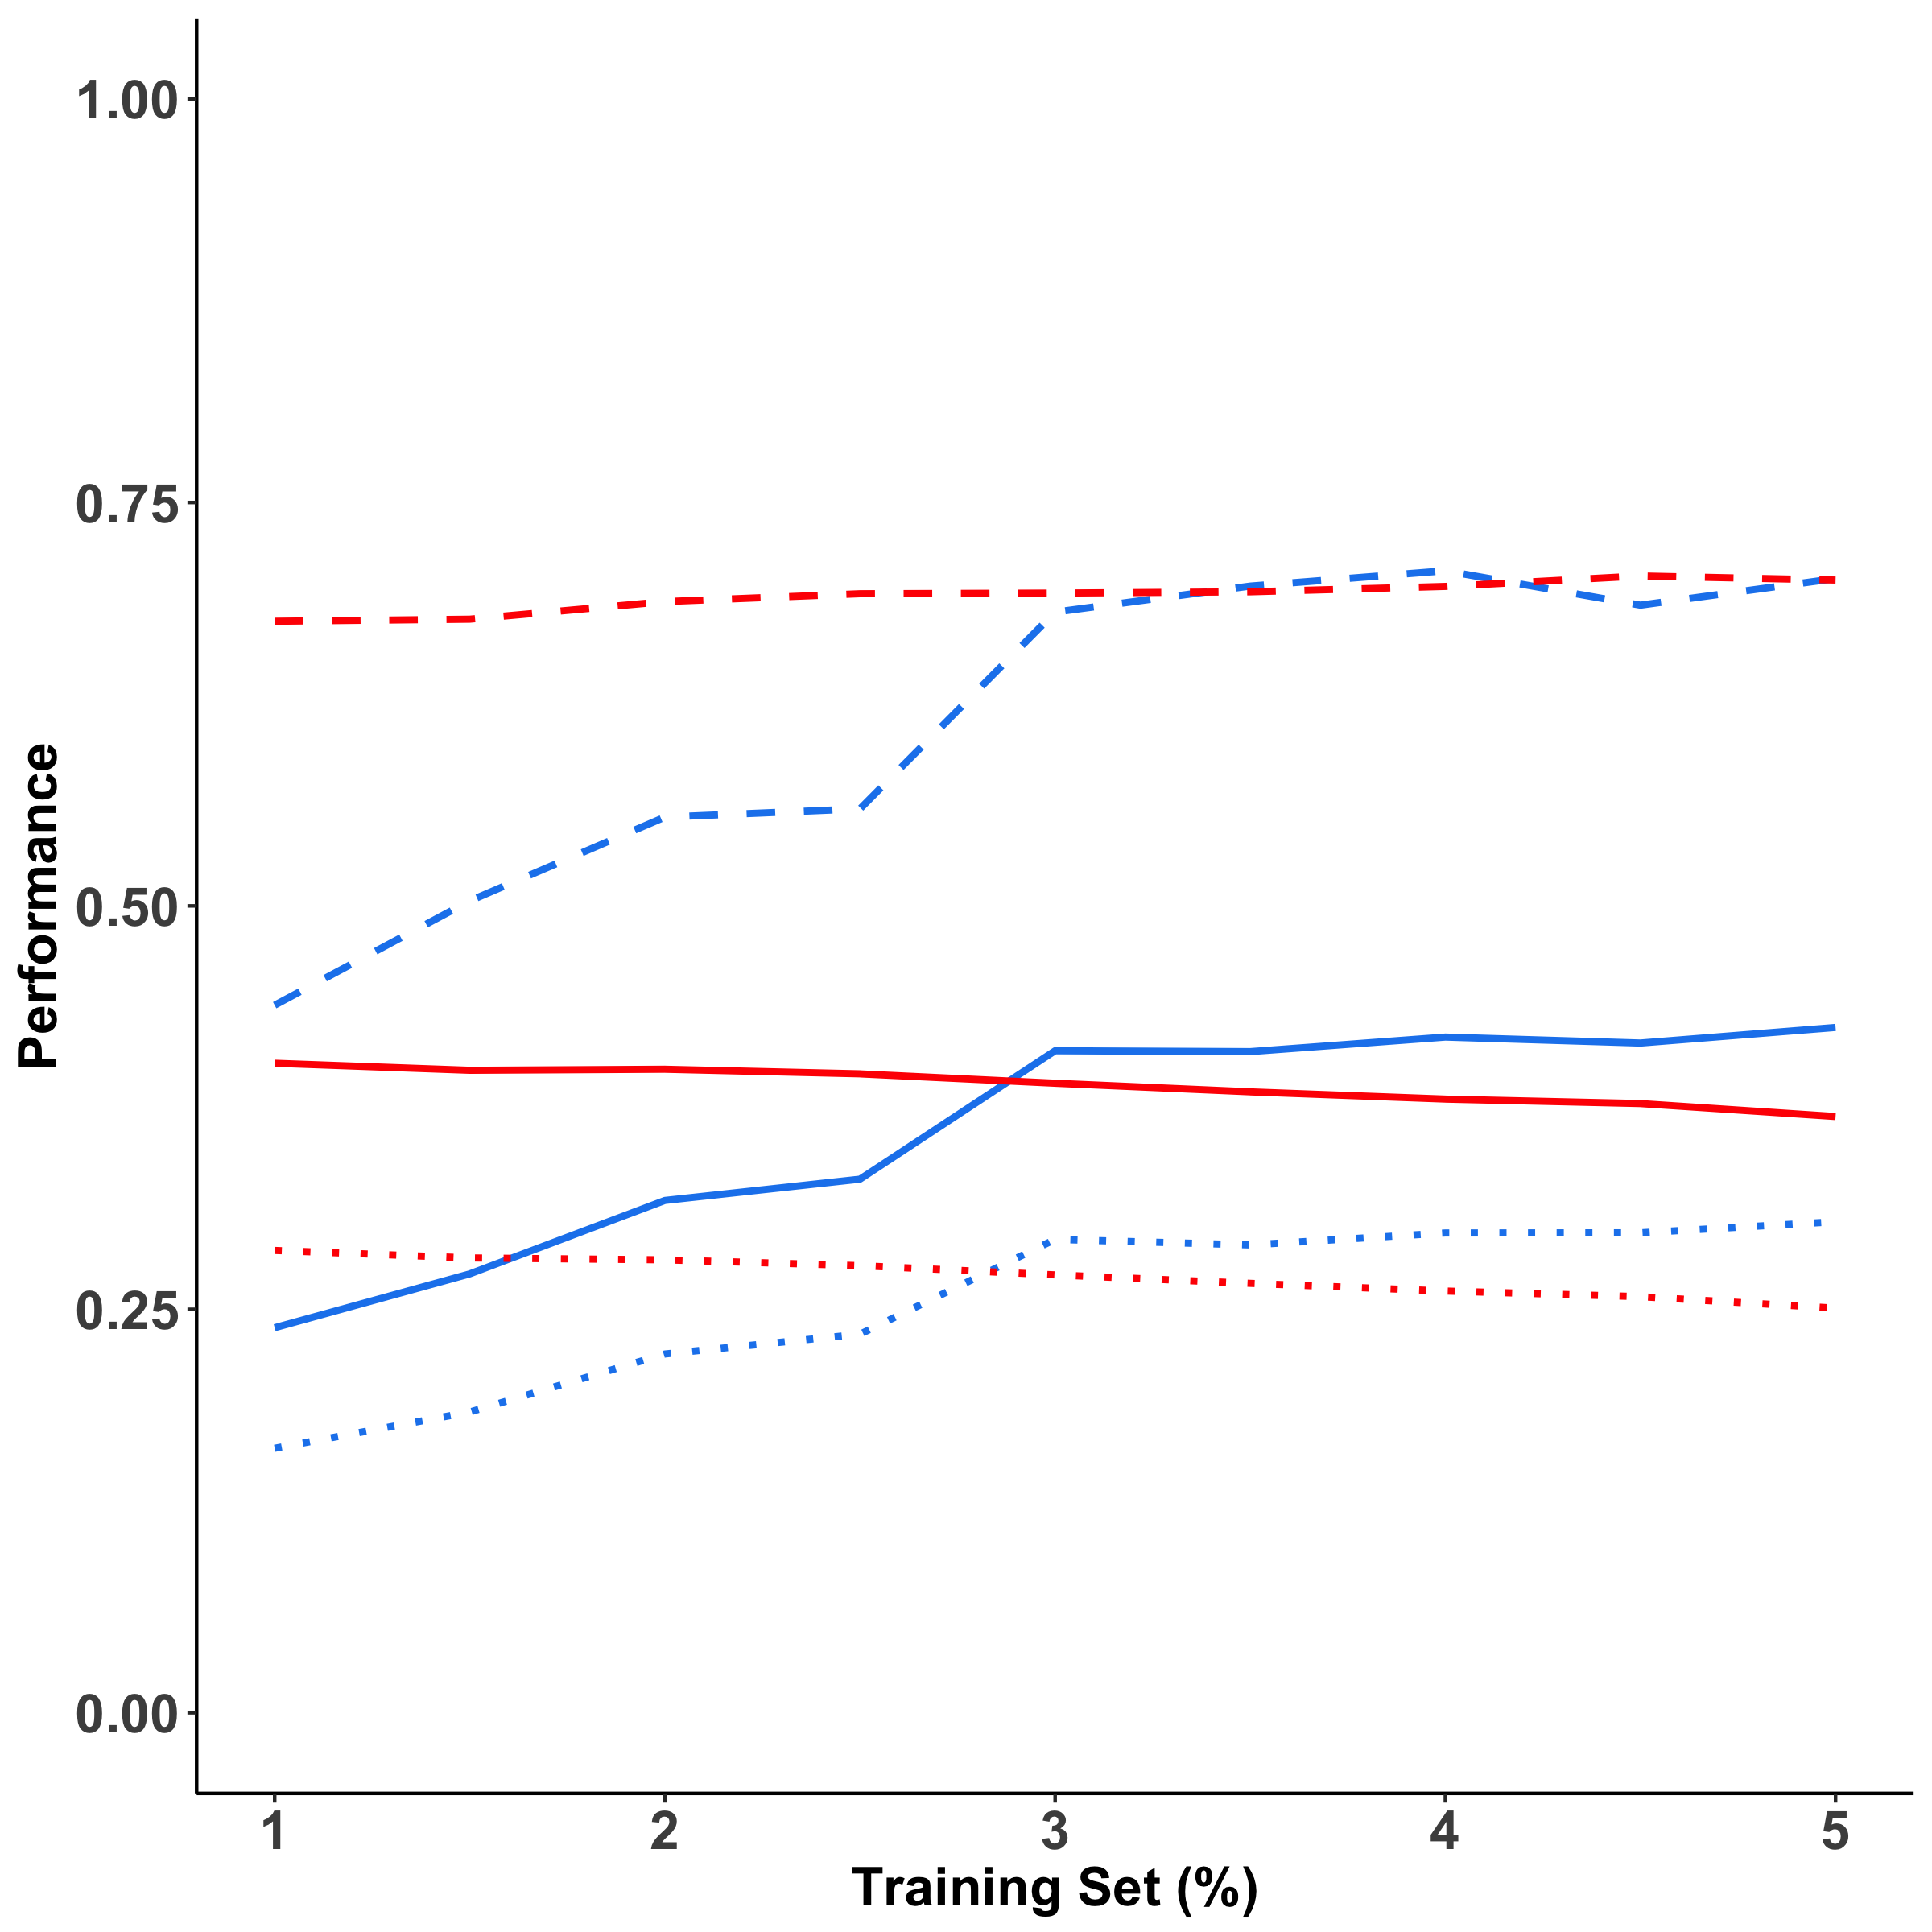
\includegraphics[width=\textwidth]{measures_median_0.png}
        \caption{Median Cutoff}
 %   \end{subfigure}
  %  \begin{subfigure}[b]{0.35\textwidth}
 %       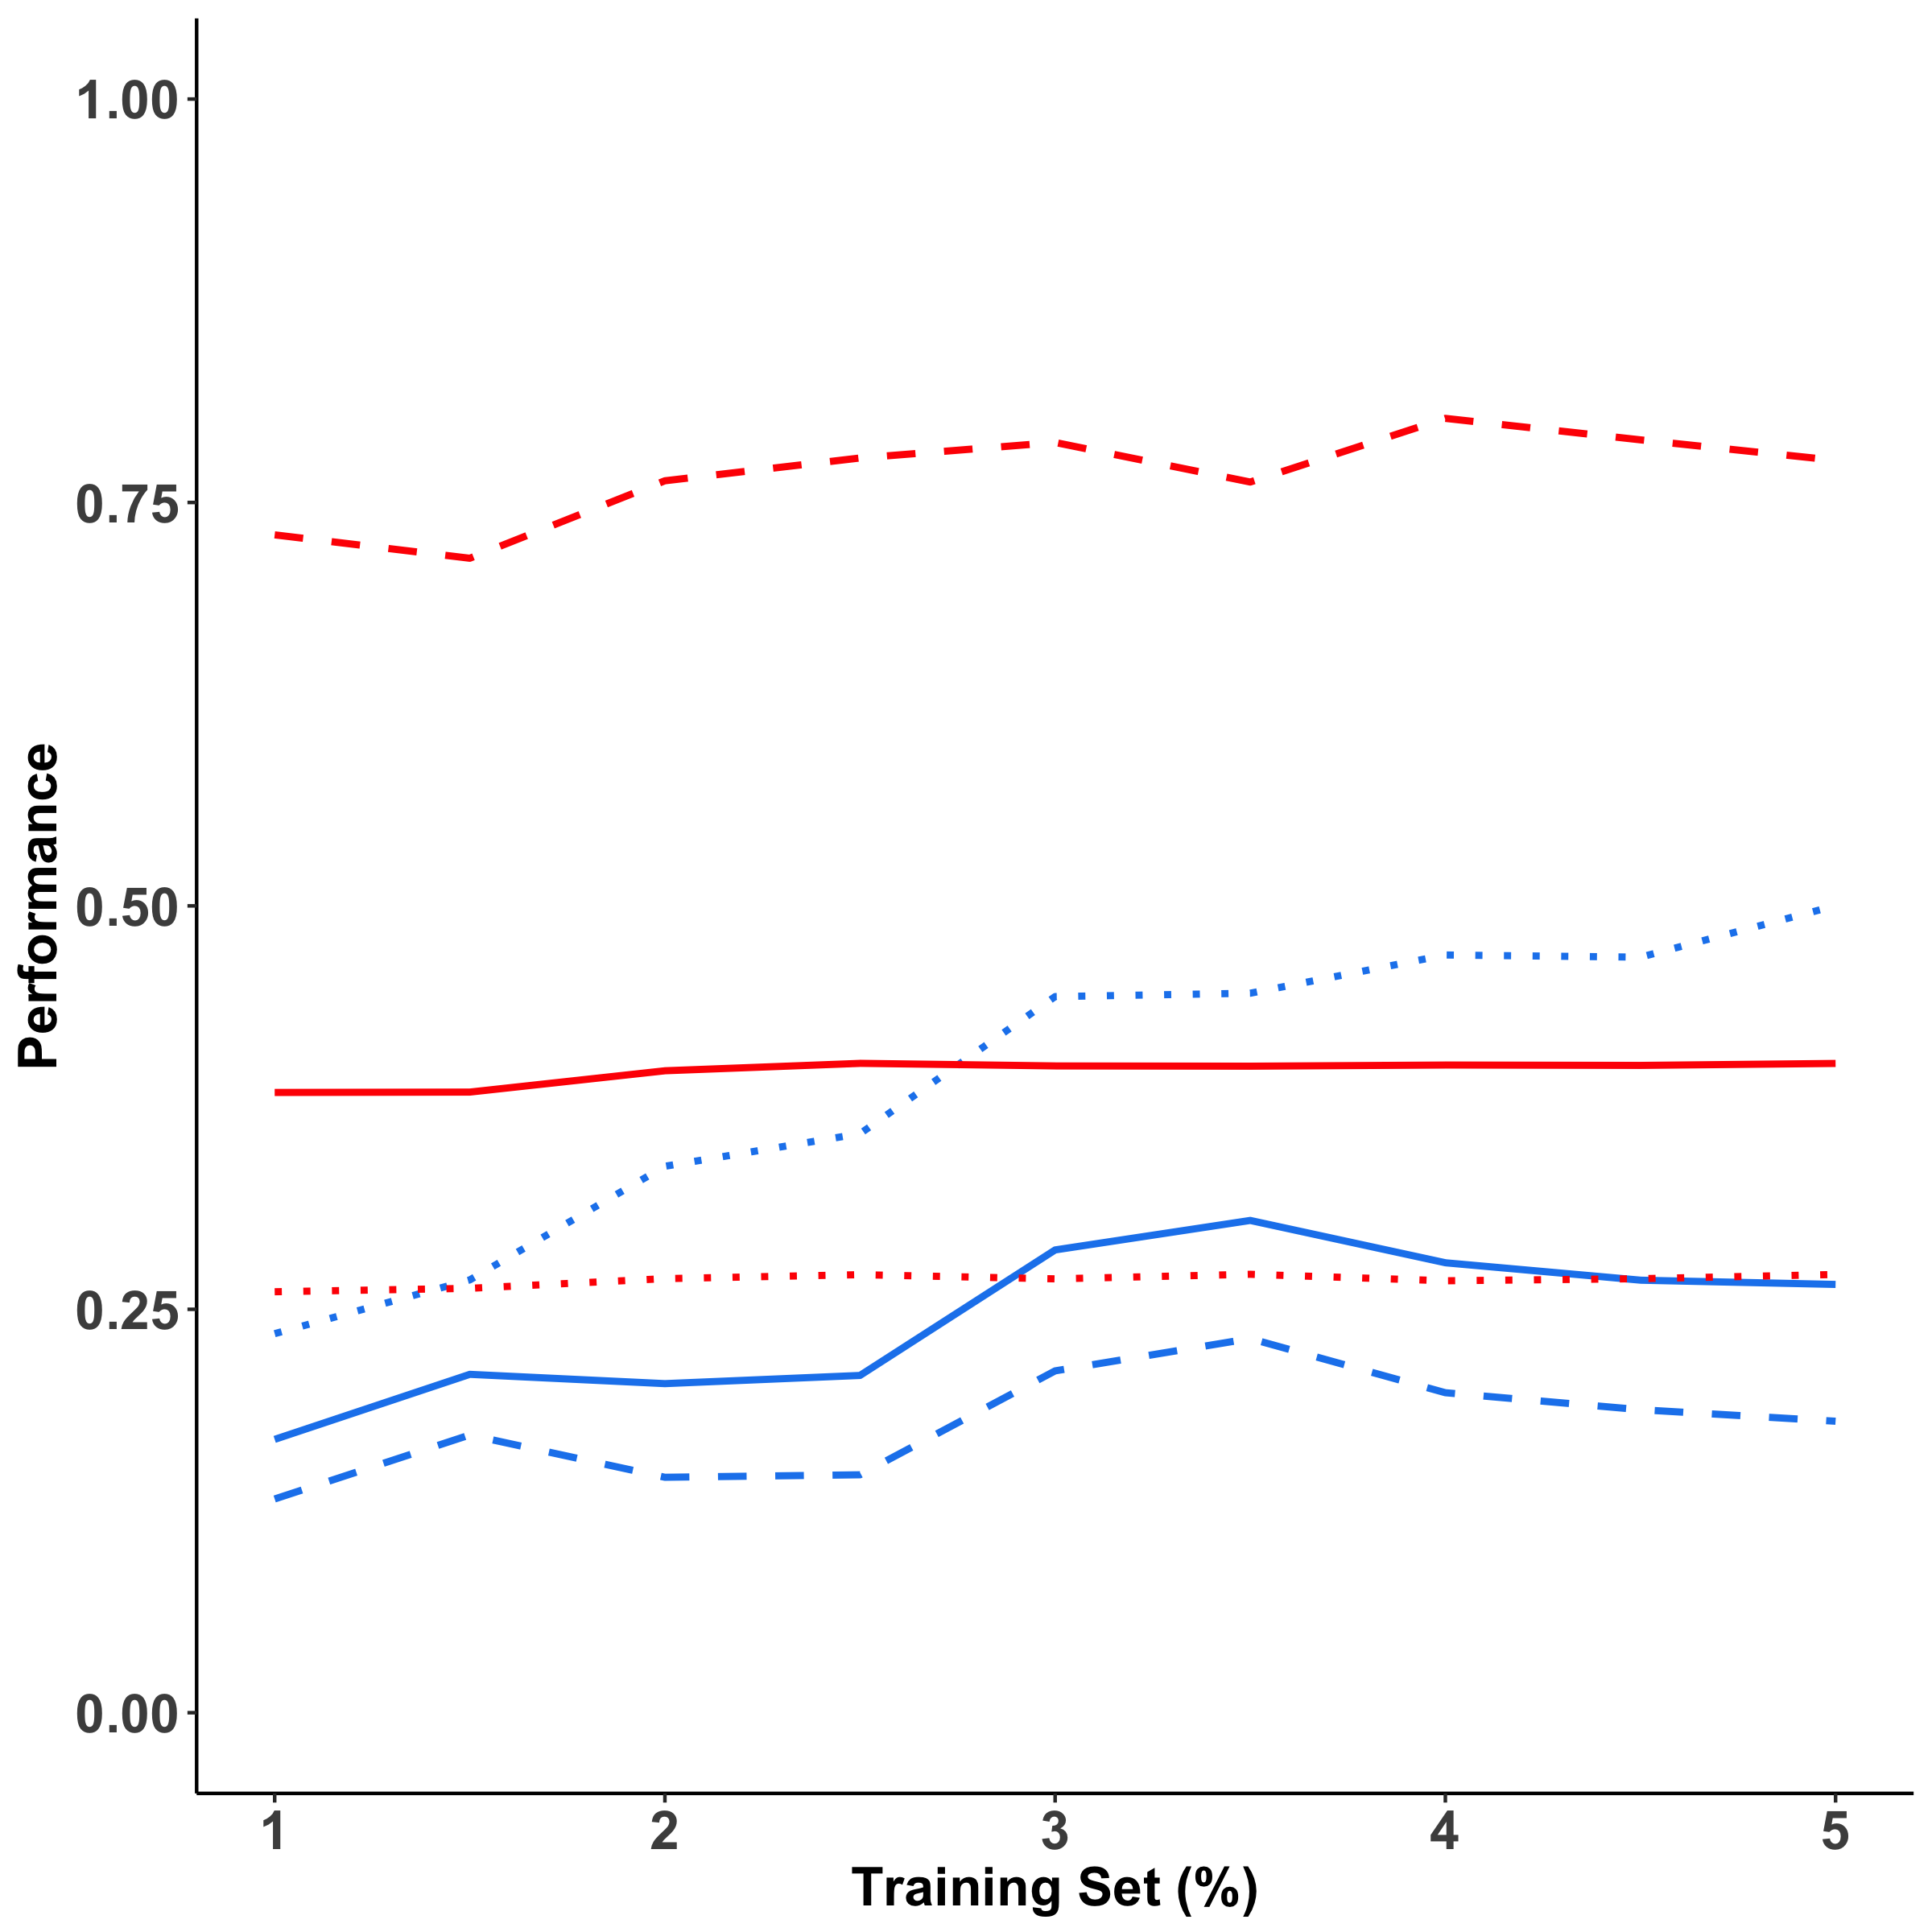
\includegraphics[width=\textwidth]{measures_pp50_0.png}
        \caption{0.50 Predicted Score Cutoff}
%    \end{subfigure}
 %   \begin{subfigure}[b]{0.35\textwidth}
%        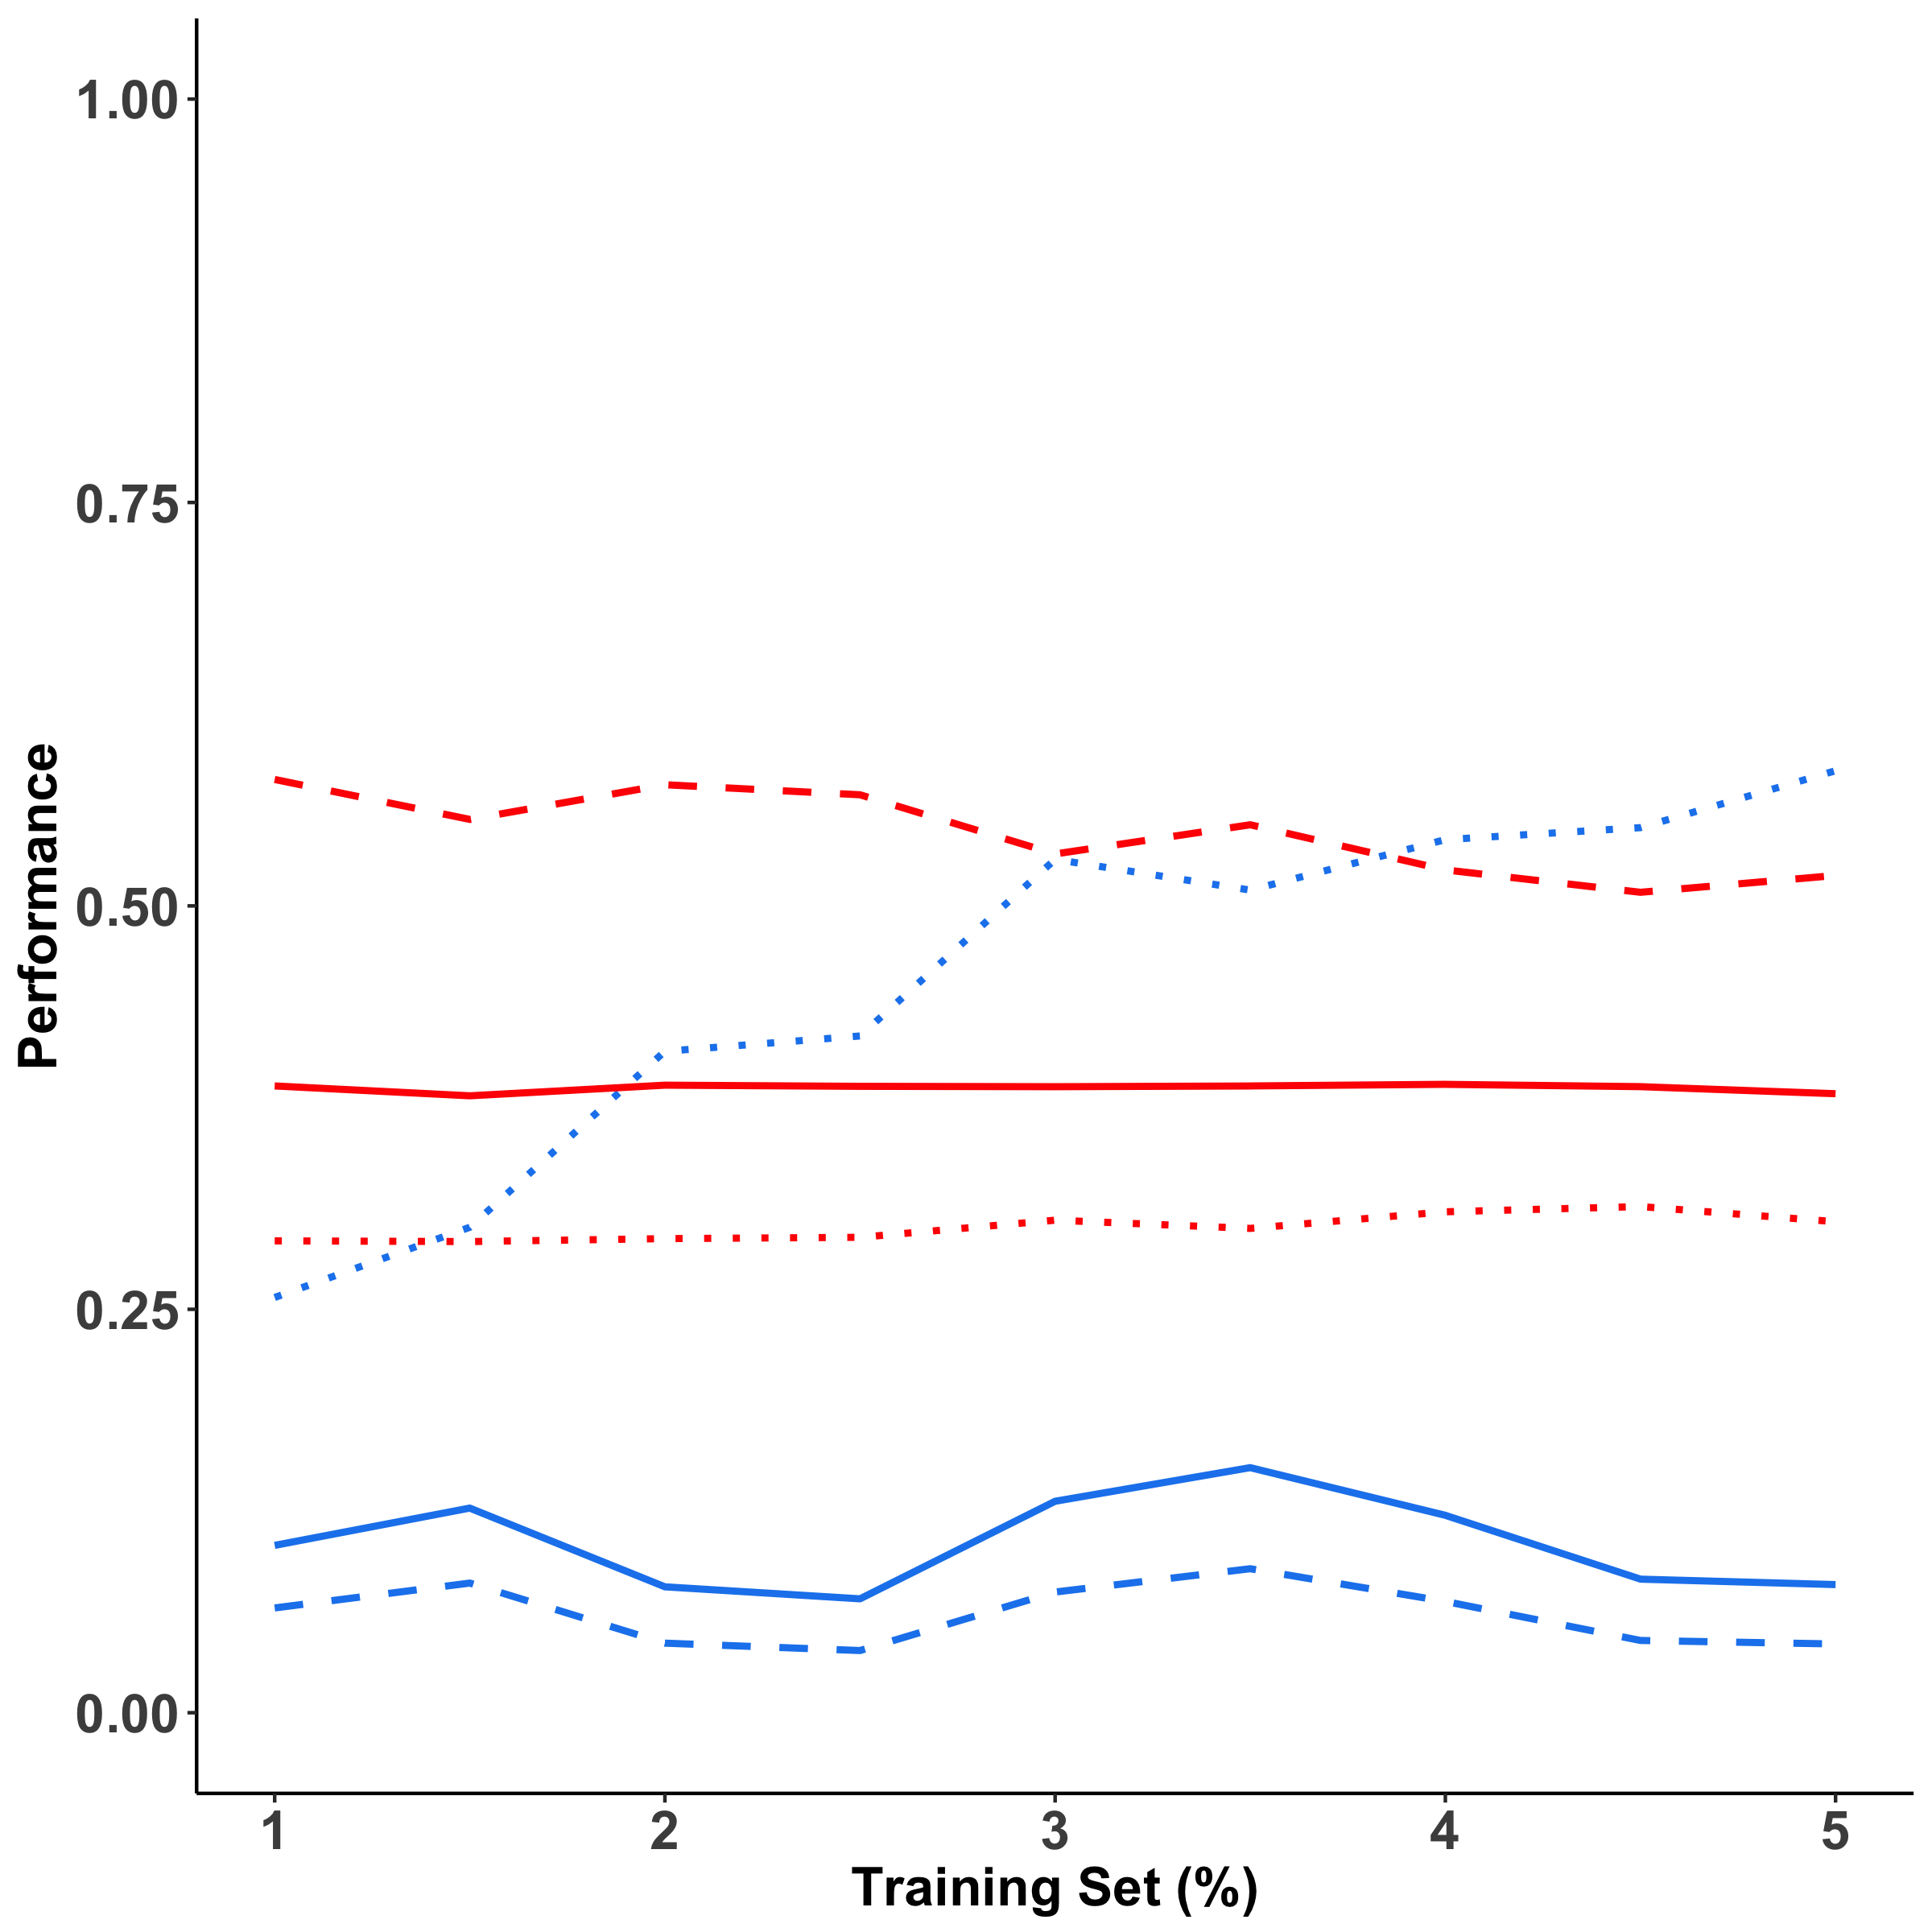
\includegraphics[width=\textwidth]{measures_pp80_0.png}
        \caption{0.80 Predicted Score Cutoff}
%    \end{subfigure}
 %   \begin{subfigure}[b]{0.35\textwidth}
%        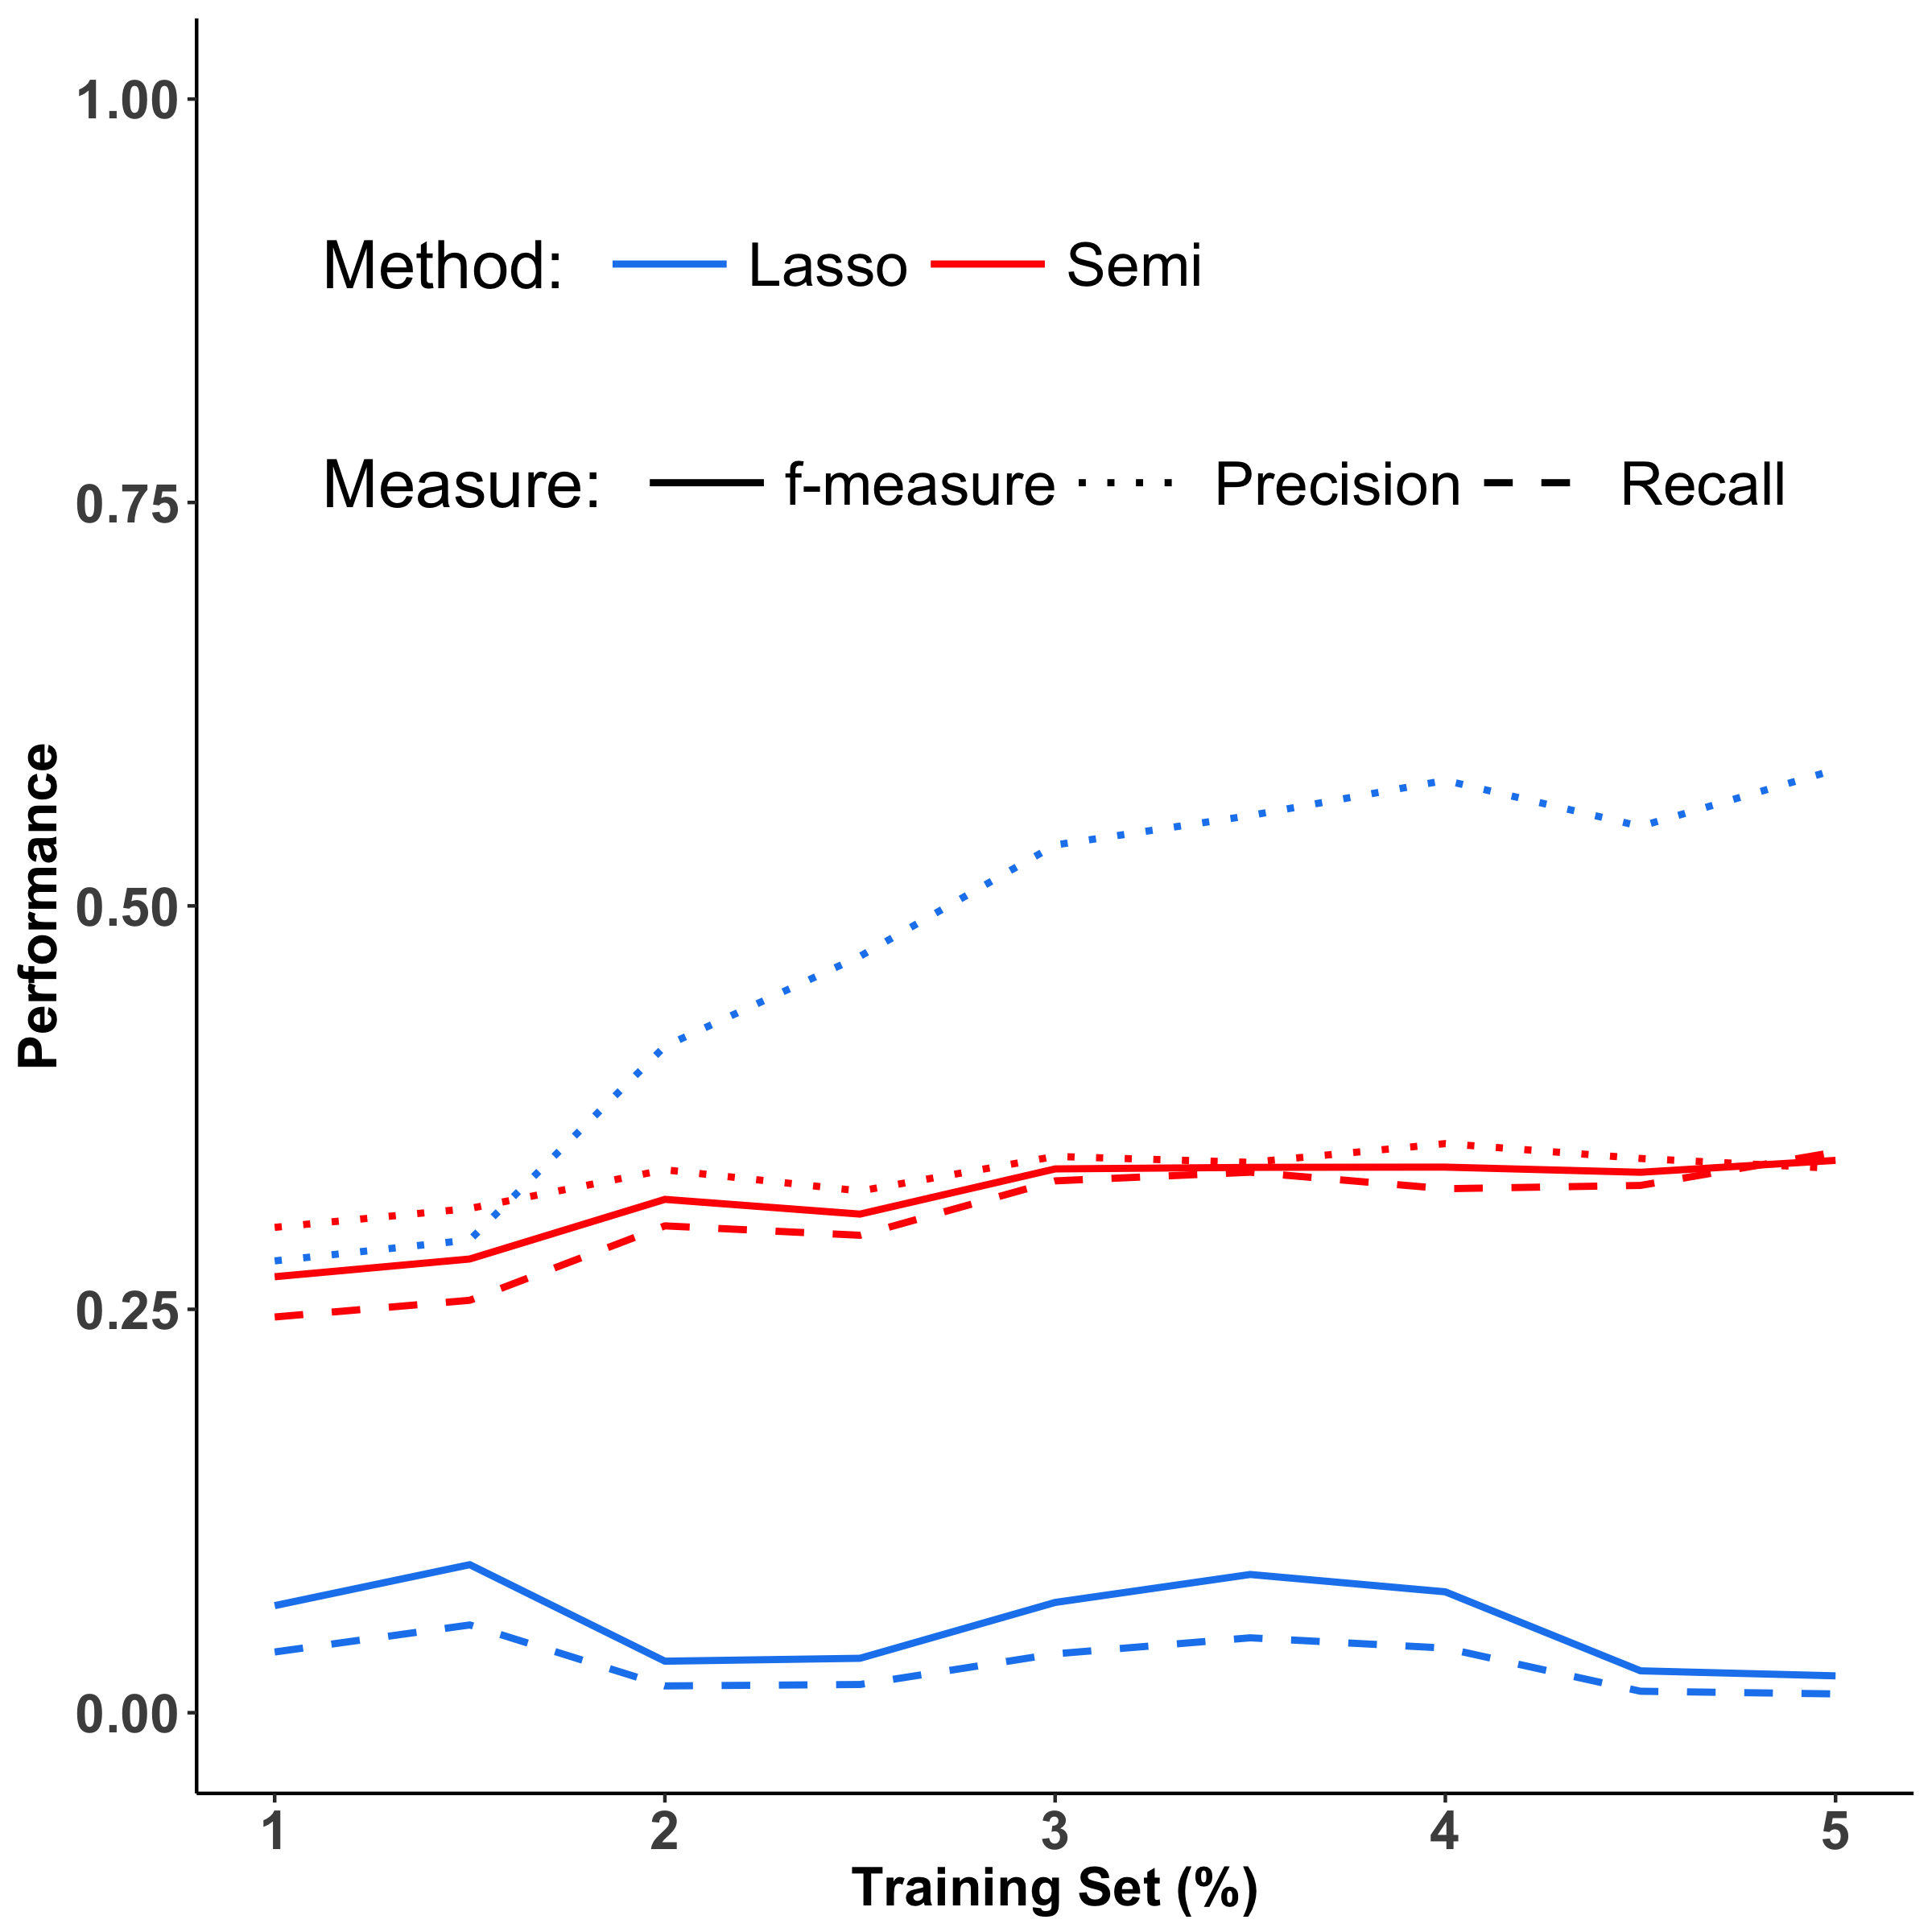
\includegraphics[width=\textwidth]{measures_pp95_0.png}
        \caption{0.95 Predicted Score Cutoff}
 %   \end{subfigure}
    \vspace{1cm}
    \caption{\textbf{Performance of Semi-supervised and LASSO methods with predicted score cutoffs at median, 0.50, 0.80, and 0.95 at 0\% contamination.} Semi-supervised method is shown in red while LASSO is shown in blue. Precision, recall, and f-measures are represented by dotted, dashed, and solid lines, respectively. The median is a relative cutoff while the other cutoffs represent absolute cutoffs with re-scaled predicted probabilities.}
    \label{fig:perf0}
\end{figure}


% Supplemental Figures
\renewcommand{\figurename}{Supplementary Figure}
\setcounter{figure}{0}

\begin{figure}[ht!]
    \centering
%    \begin{subfigure}[b]{0.6\textwidth}
%        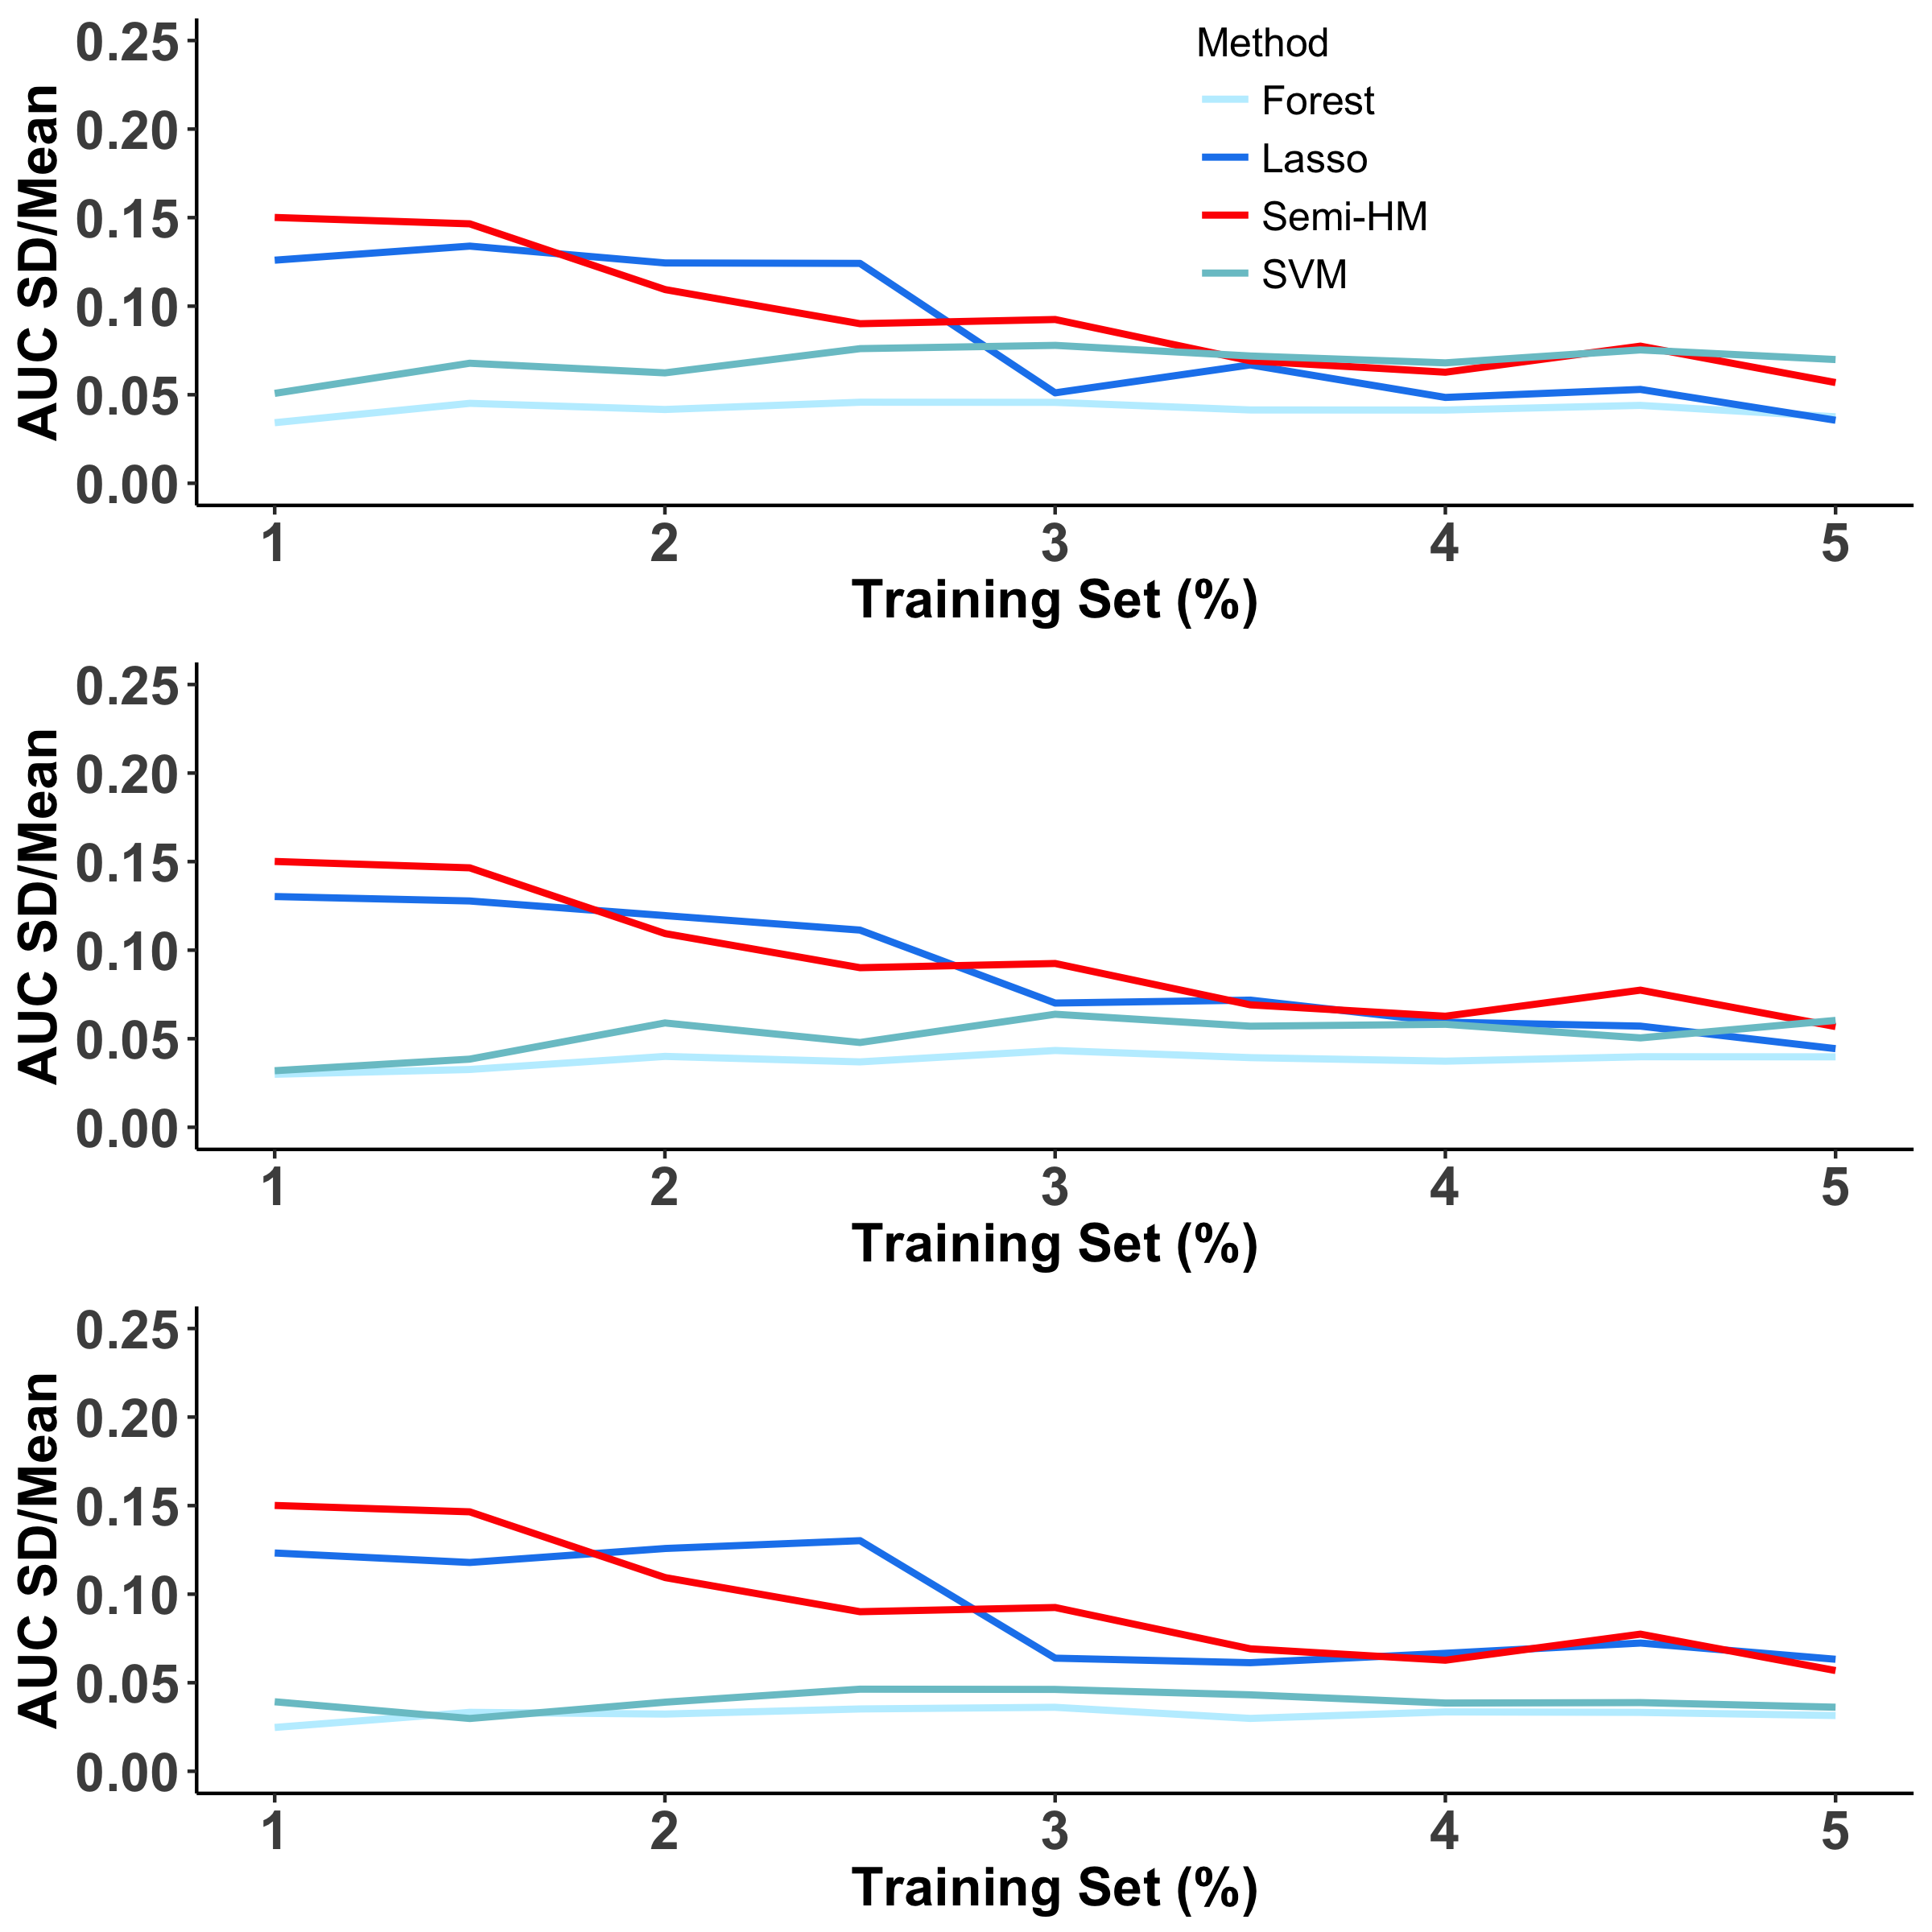
\includegraphics[width=\textwidth]{AUCcvmean.png}
        \caption{AUC SD/mean}
 %   \end{subfigure}
 %   \begin{subfigure}[b]{0.45\textwidth}
%        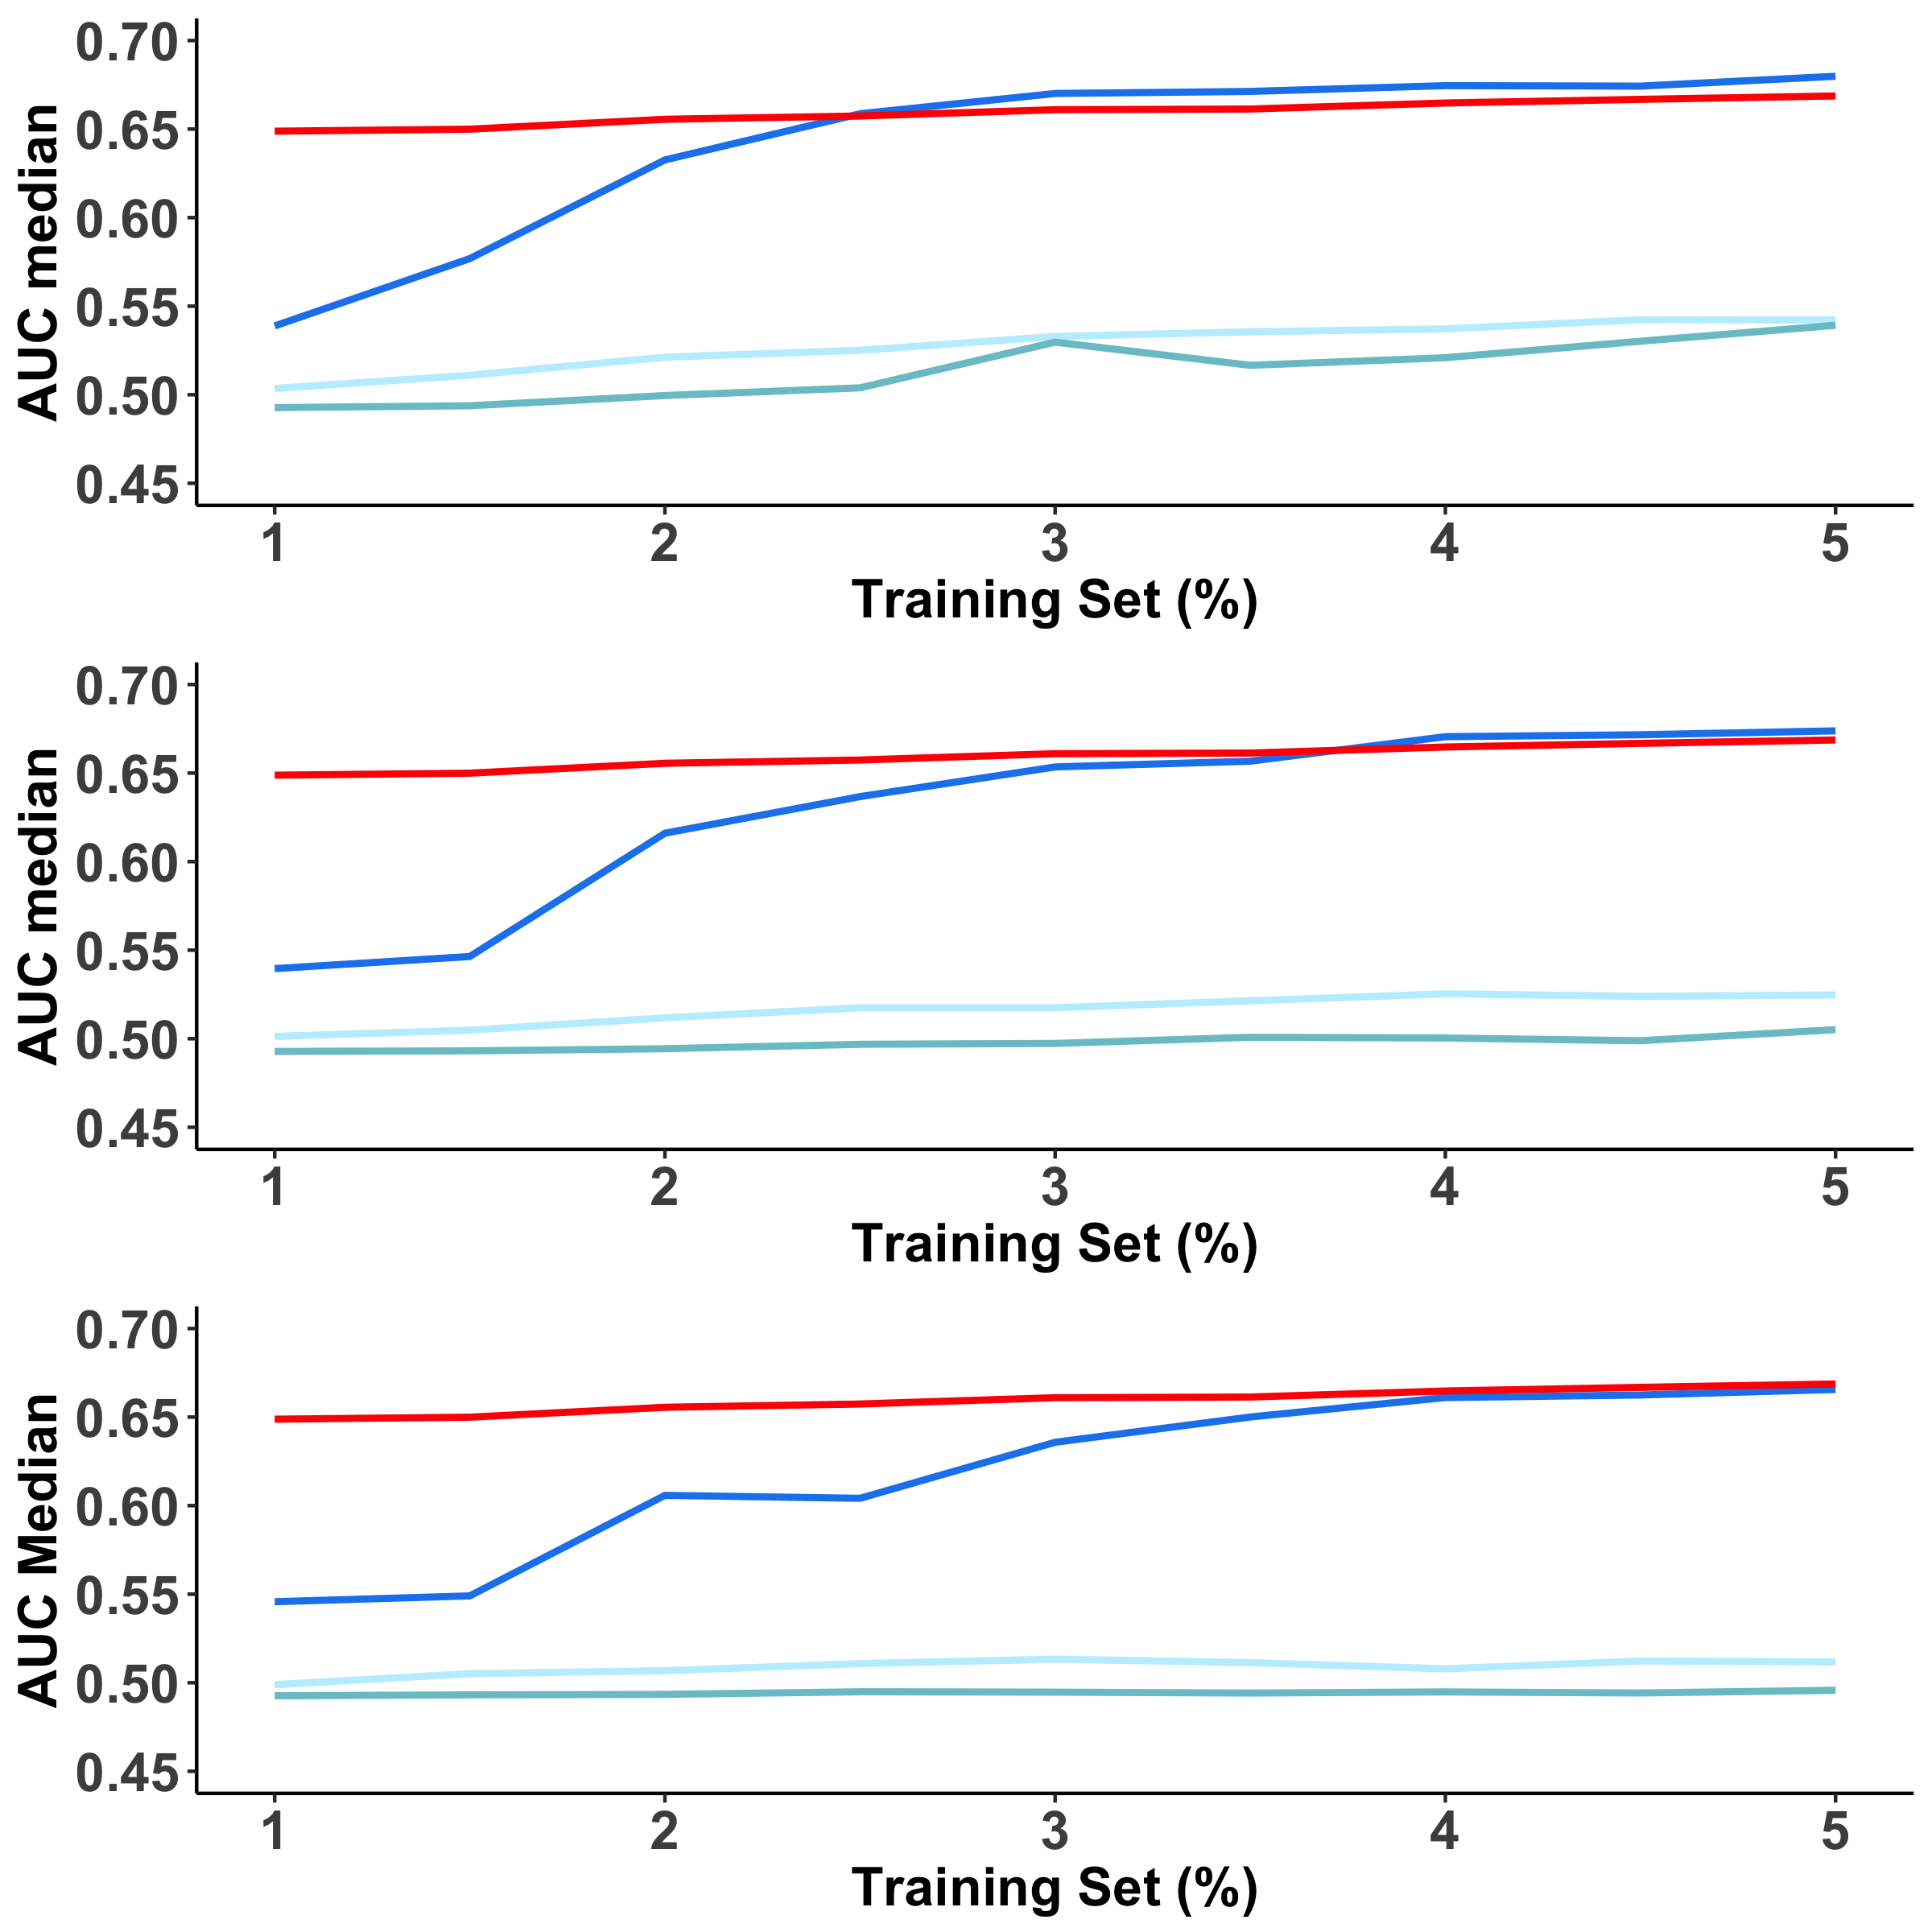
\includegraphics[width=\textwidth]{AUCmed.png} 
        \caption{AUC Mean}
 %   \end{subfigure}
%    \begin{subfigure}[b]{0.45\textwidth}
%        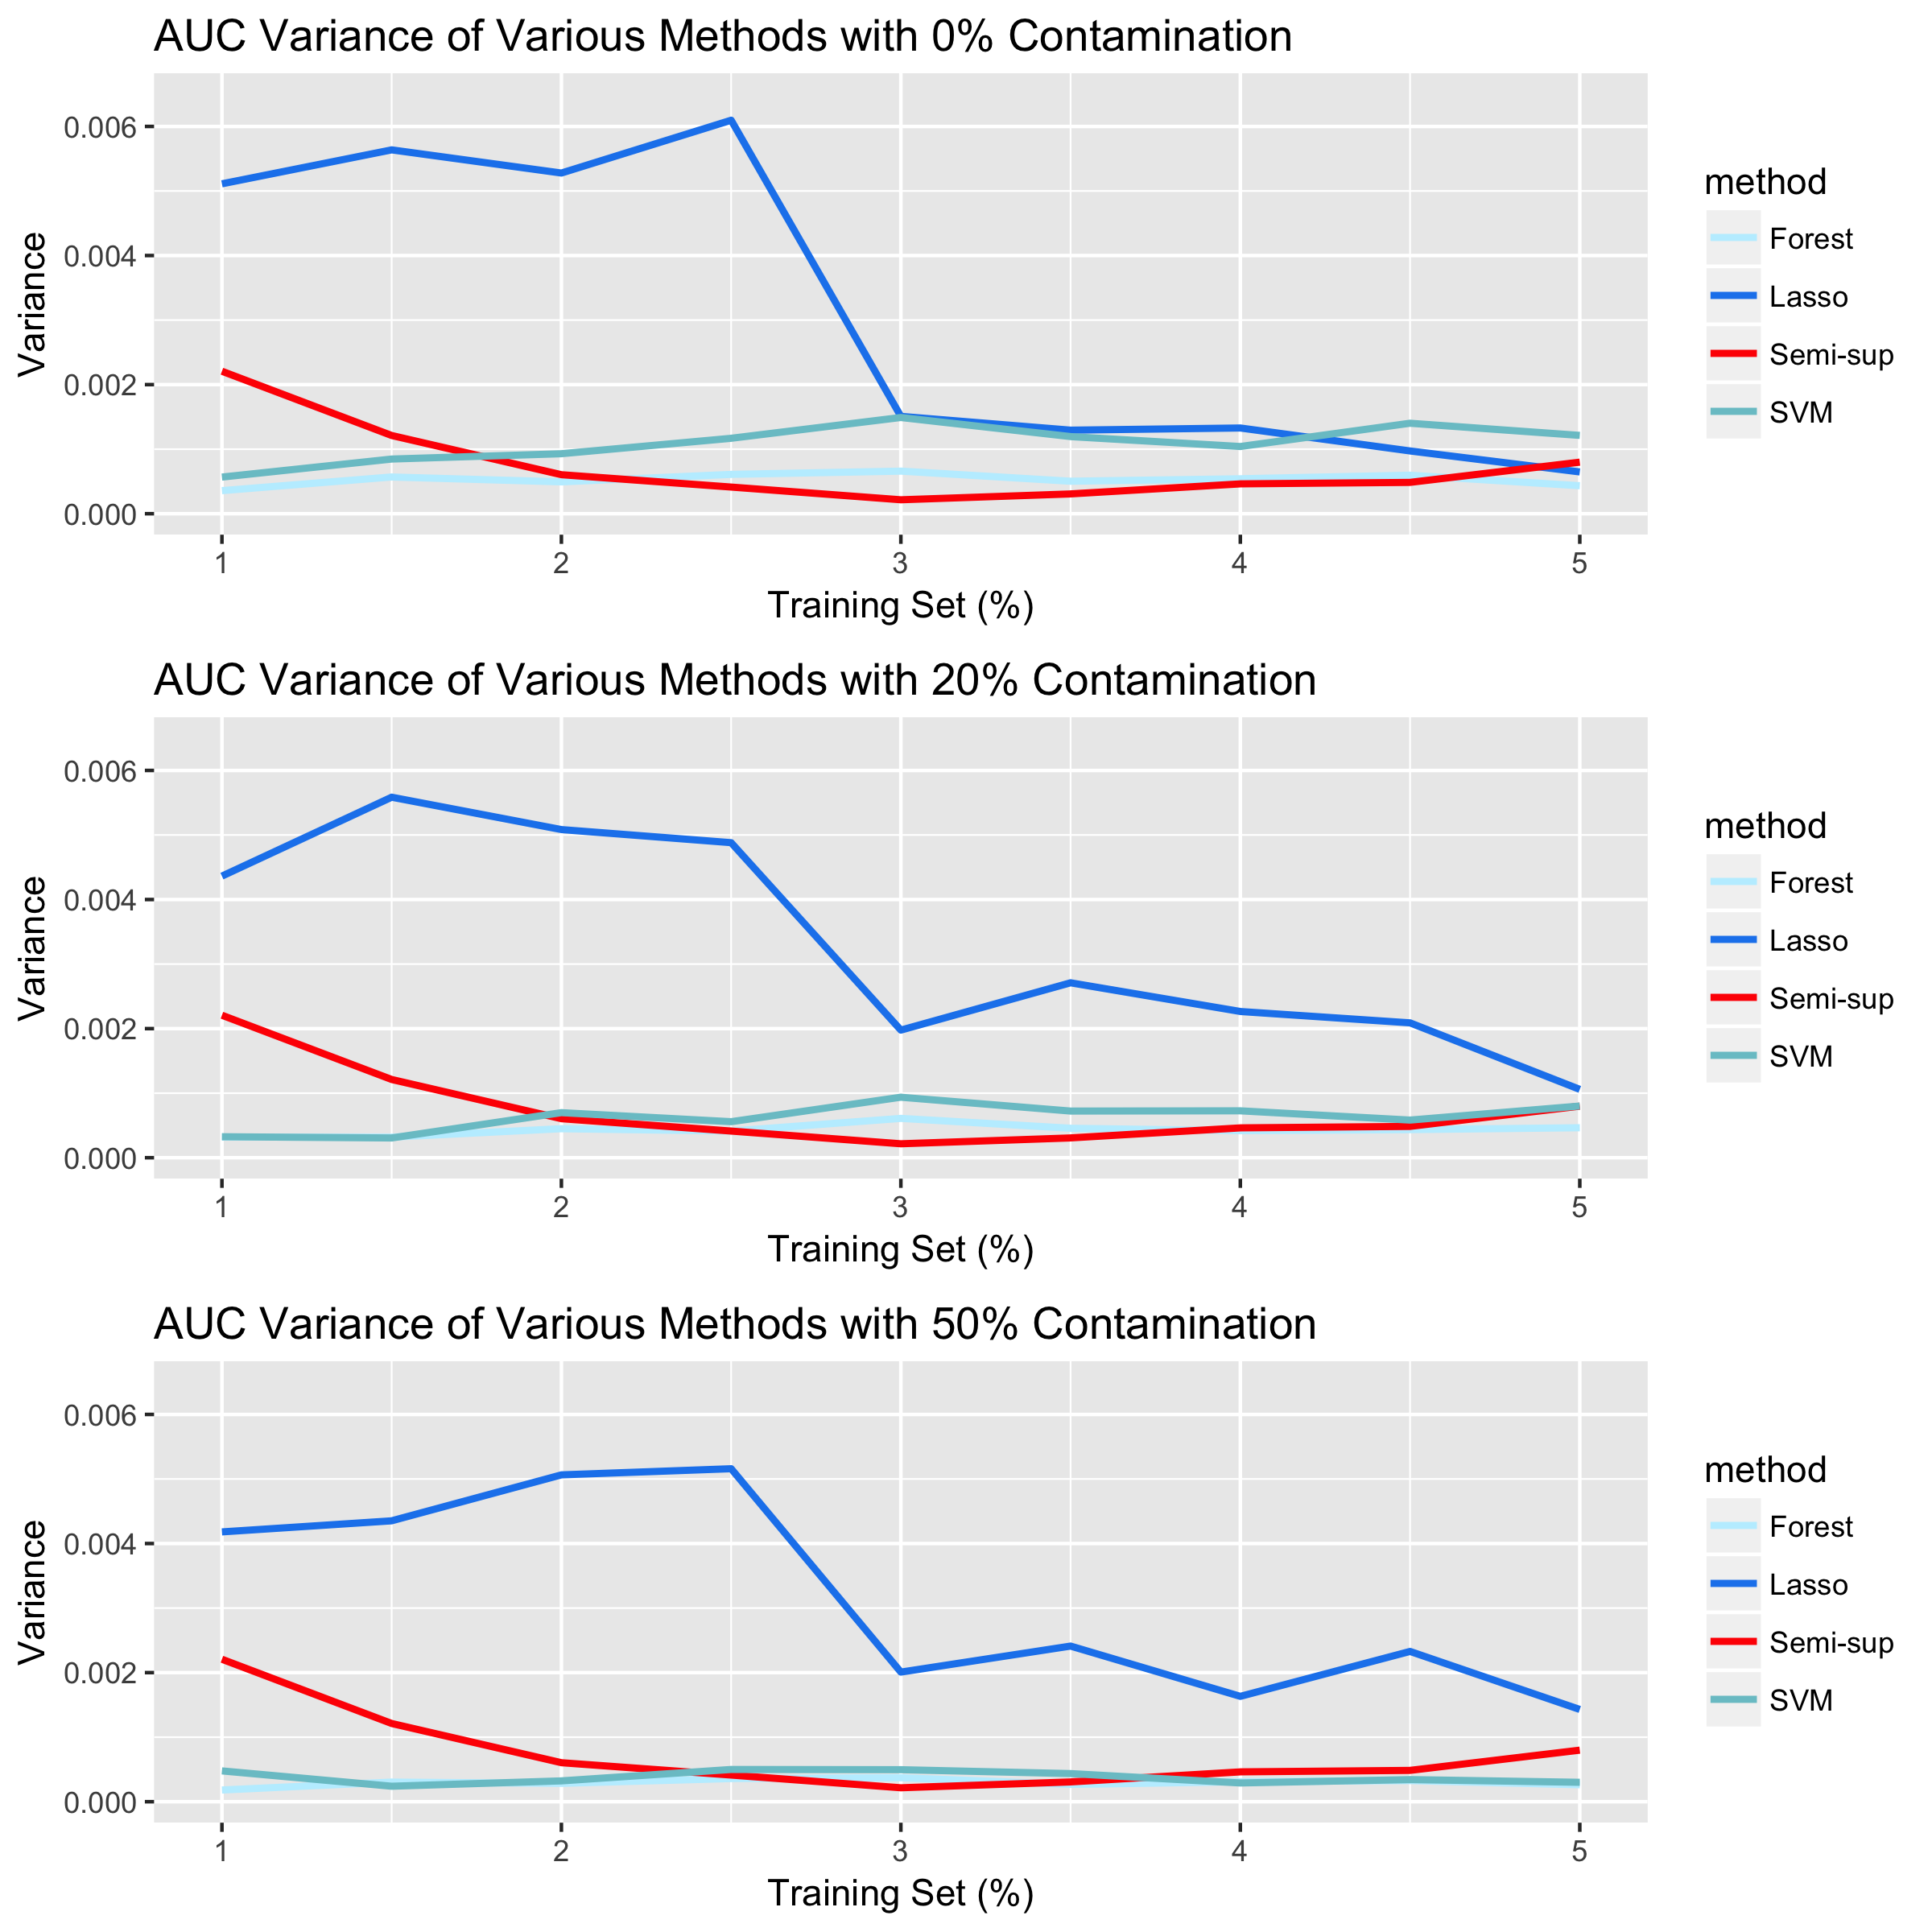
\includegraphics[width=\textwidth]{AUCvariances.png} 
        \caption{AUC Variance}
%    \end{subfigure}
    \vspace{1cm}
    \caption{\textbf{Evaluation of summary statistics comparing semi-supervised and supervised methods.} 100 iterations were executed at training sets (1\%, 1.5\%, 2\%,...,5\%) for all four methods and negative contamination levels (0\%, 20\%, and 50\%). Semi-supervised method is shown in red while the supervised methods (LASSO, SVM, and Random Forest) are shown in blue, aquamarine, and light blue, respectively. The AUC mean (a), variance (b), and CV (c) contrasts the four methods at each training set size across three contamination rates. CV is calculated as the Median Absolute Deviation (MAD) / Median}
    \label{fig:AUCsummarymean}
\end{figure}


\begin{figure}[ht]
    \centering
%    \begin{subfigure}[b]{0.35\textwidth}
%        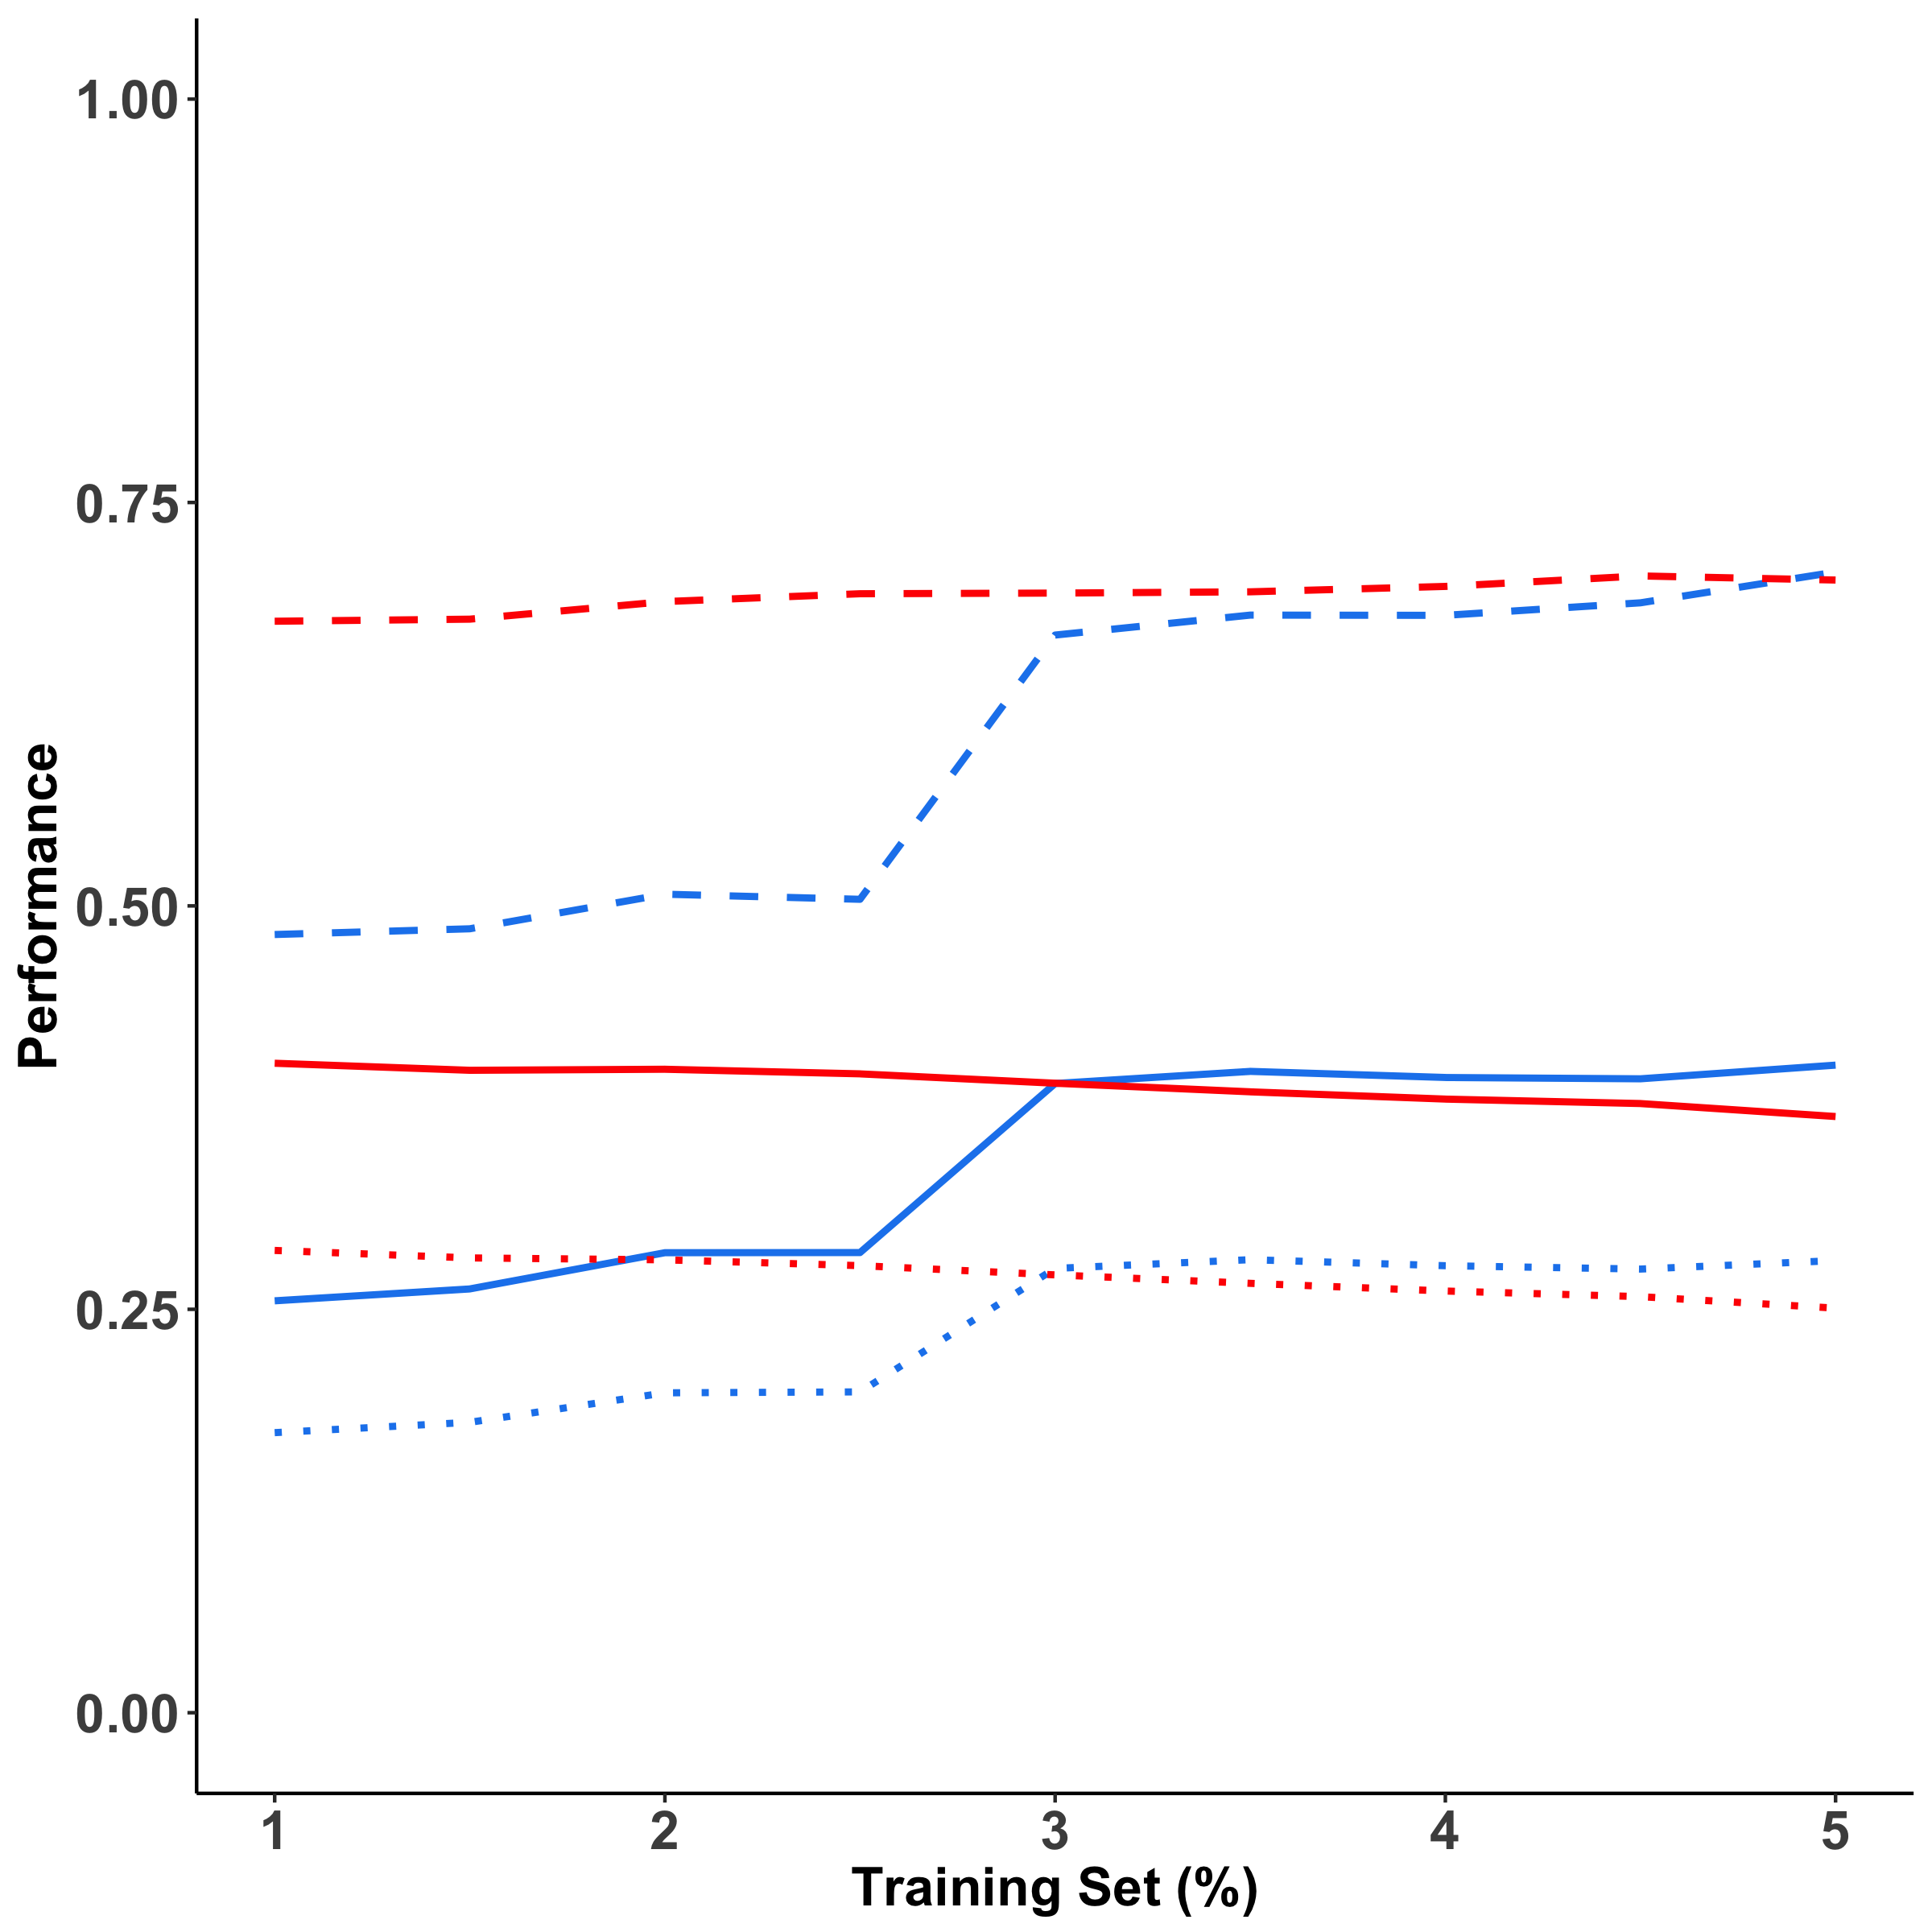
\includegraphics[width=\textwidth]{measures_median_20.png}
        \caption{Median Cutoff}
 %   \end{subfigure}
%    \begin{subfigure}[b]{0.35\textwidth}
%        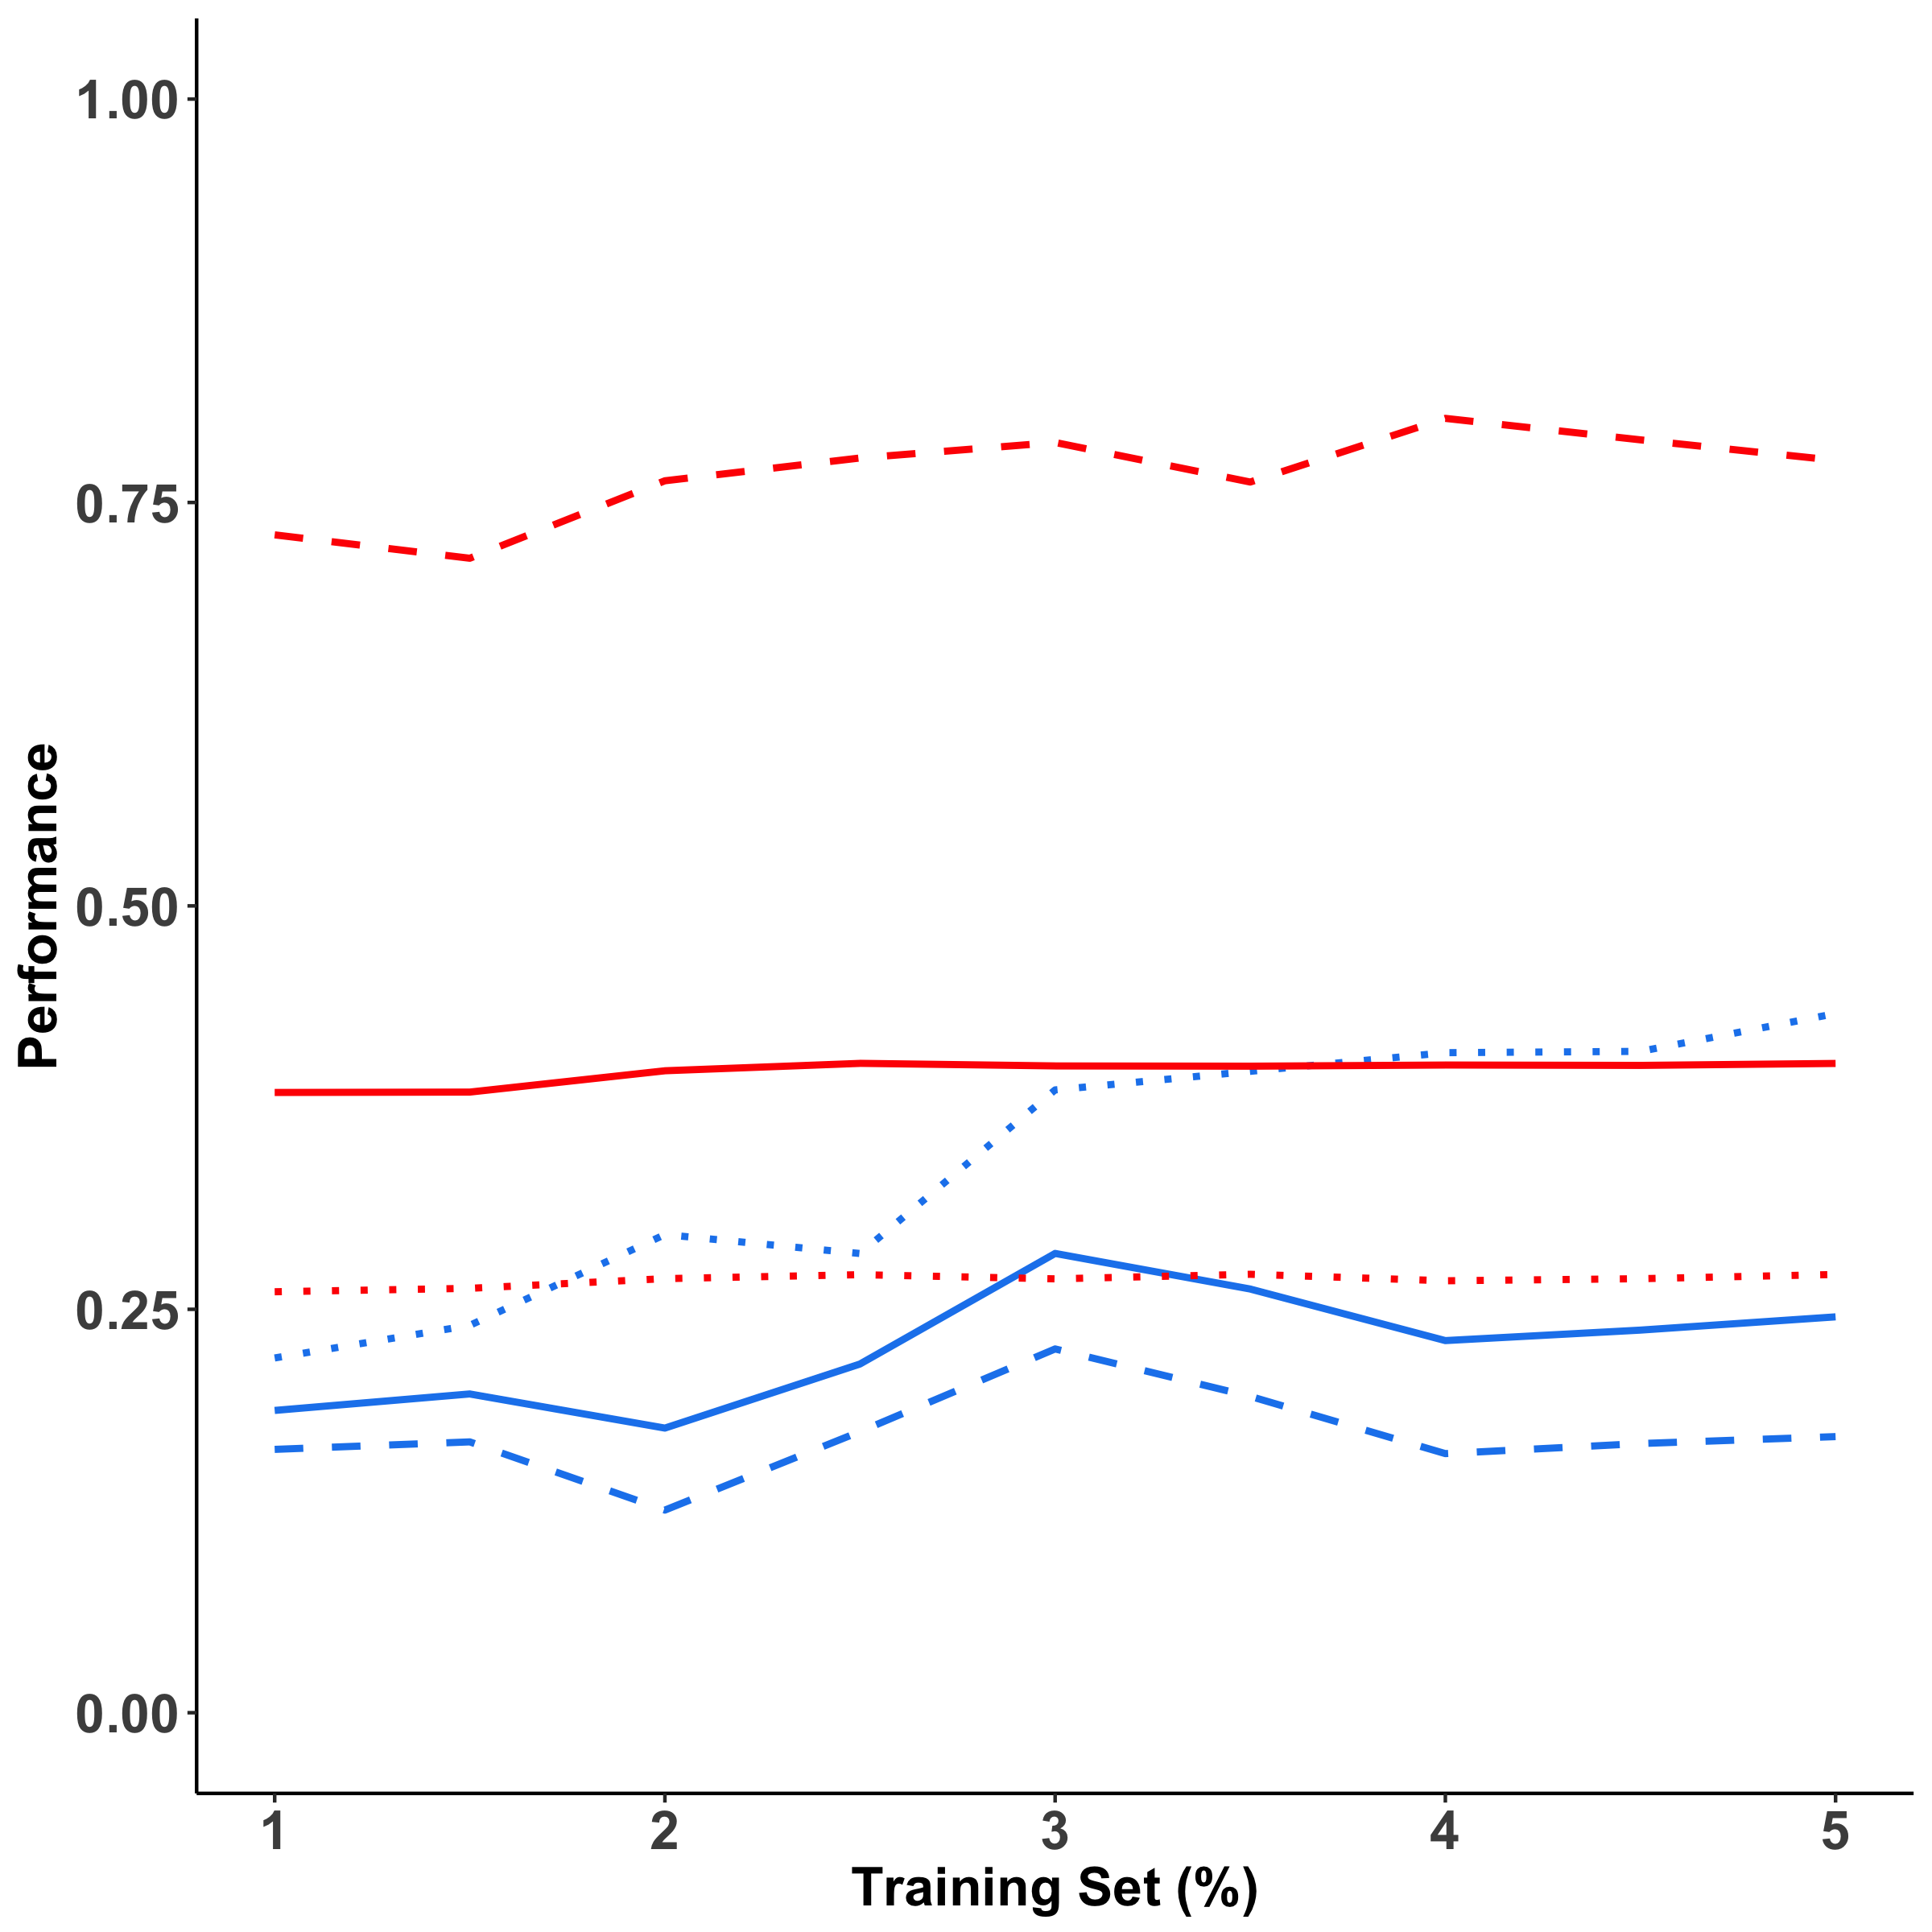
\includegraphics[width=\textwidth]{measures_pp50_20.png}
        \caption{0.50 Predicted Score Cutoff}
 %   \end{subfigure}
%    \begin{subfigure}[b]{0.35\textwidth}
%        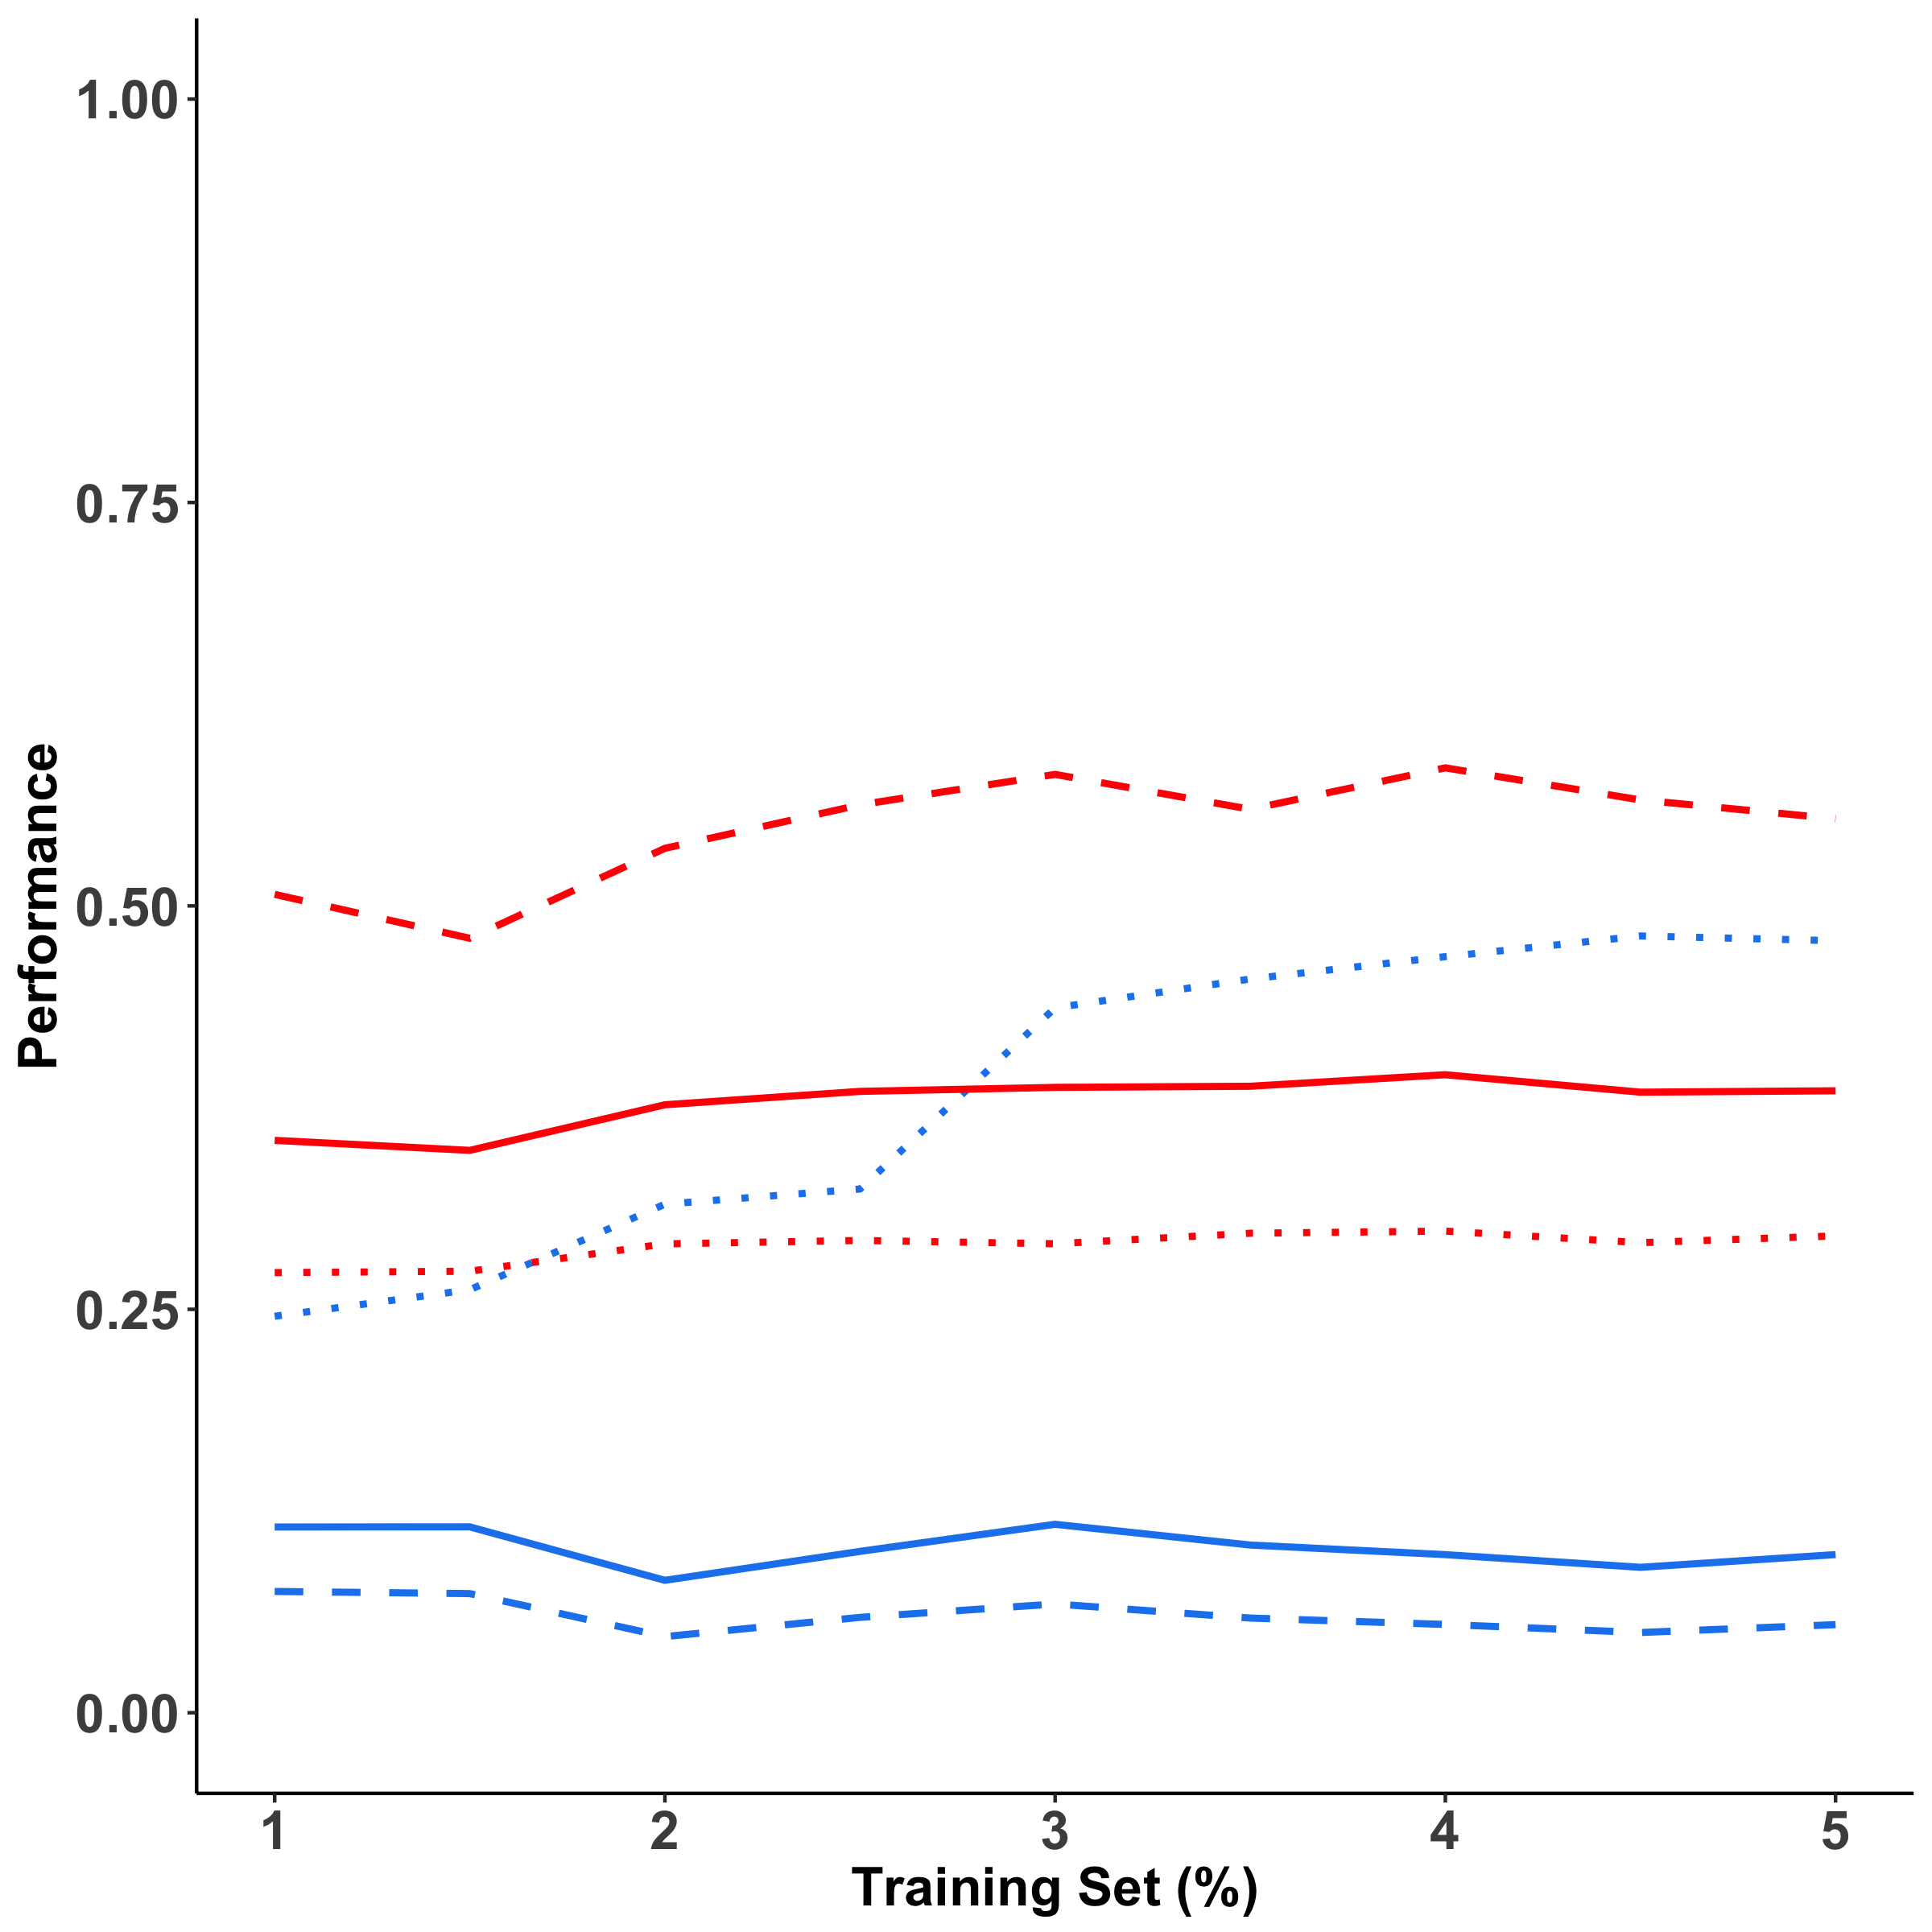
\includegraphics[width=\textwidth]{measures_pp80_20.png}
        \caption{0.80 Predicted Score Cutoff}
  %  \end{subfigure}
 %   \begin{subfigure}[b]{0.35\textwidth}
%        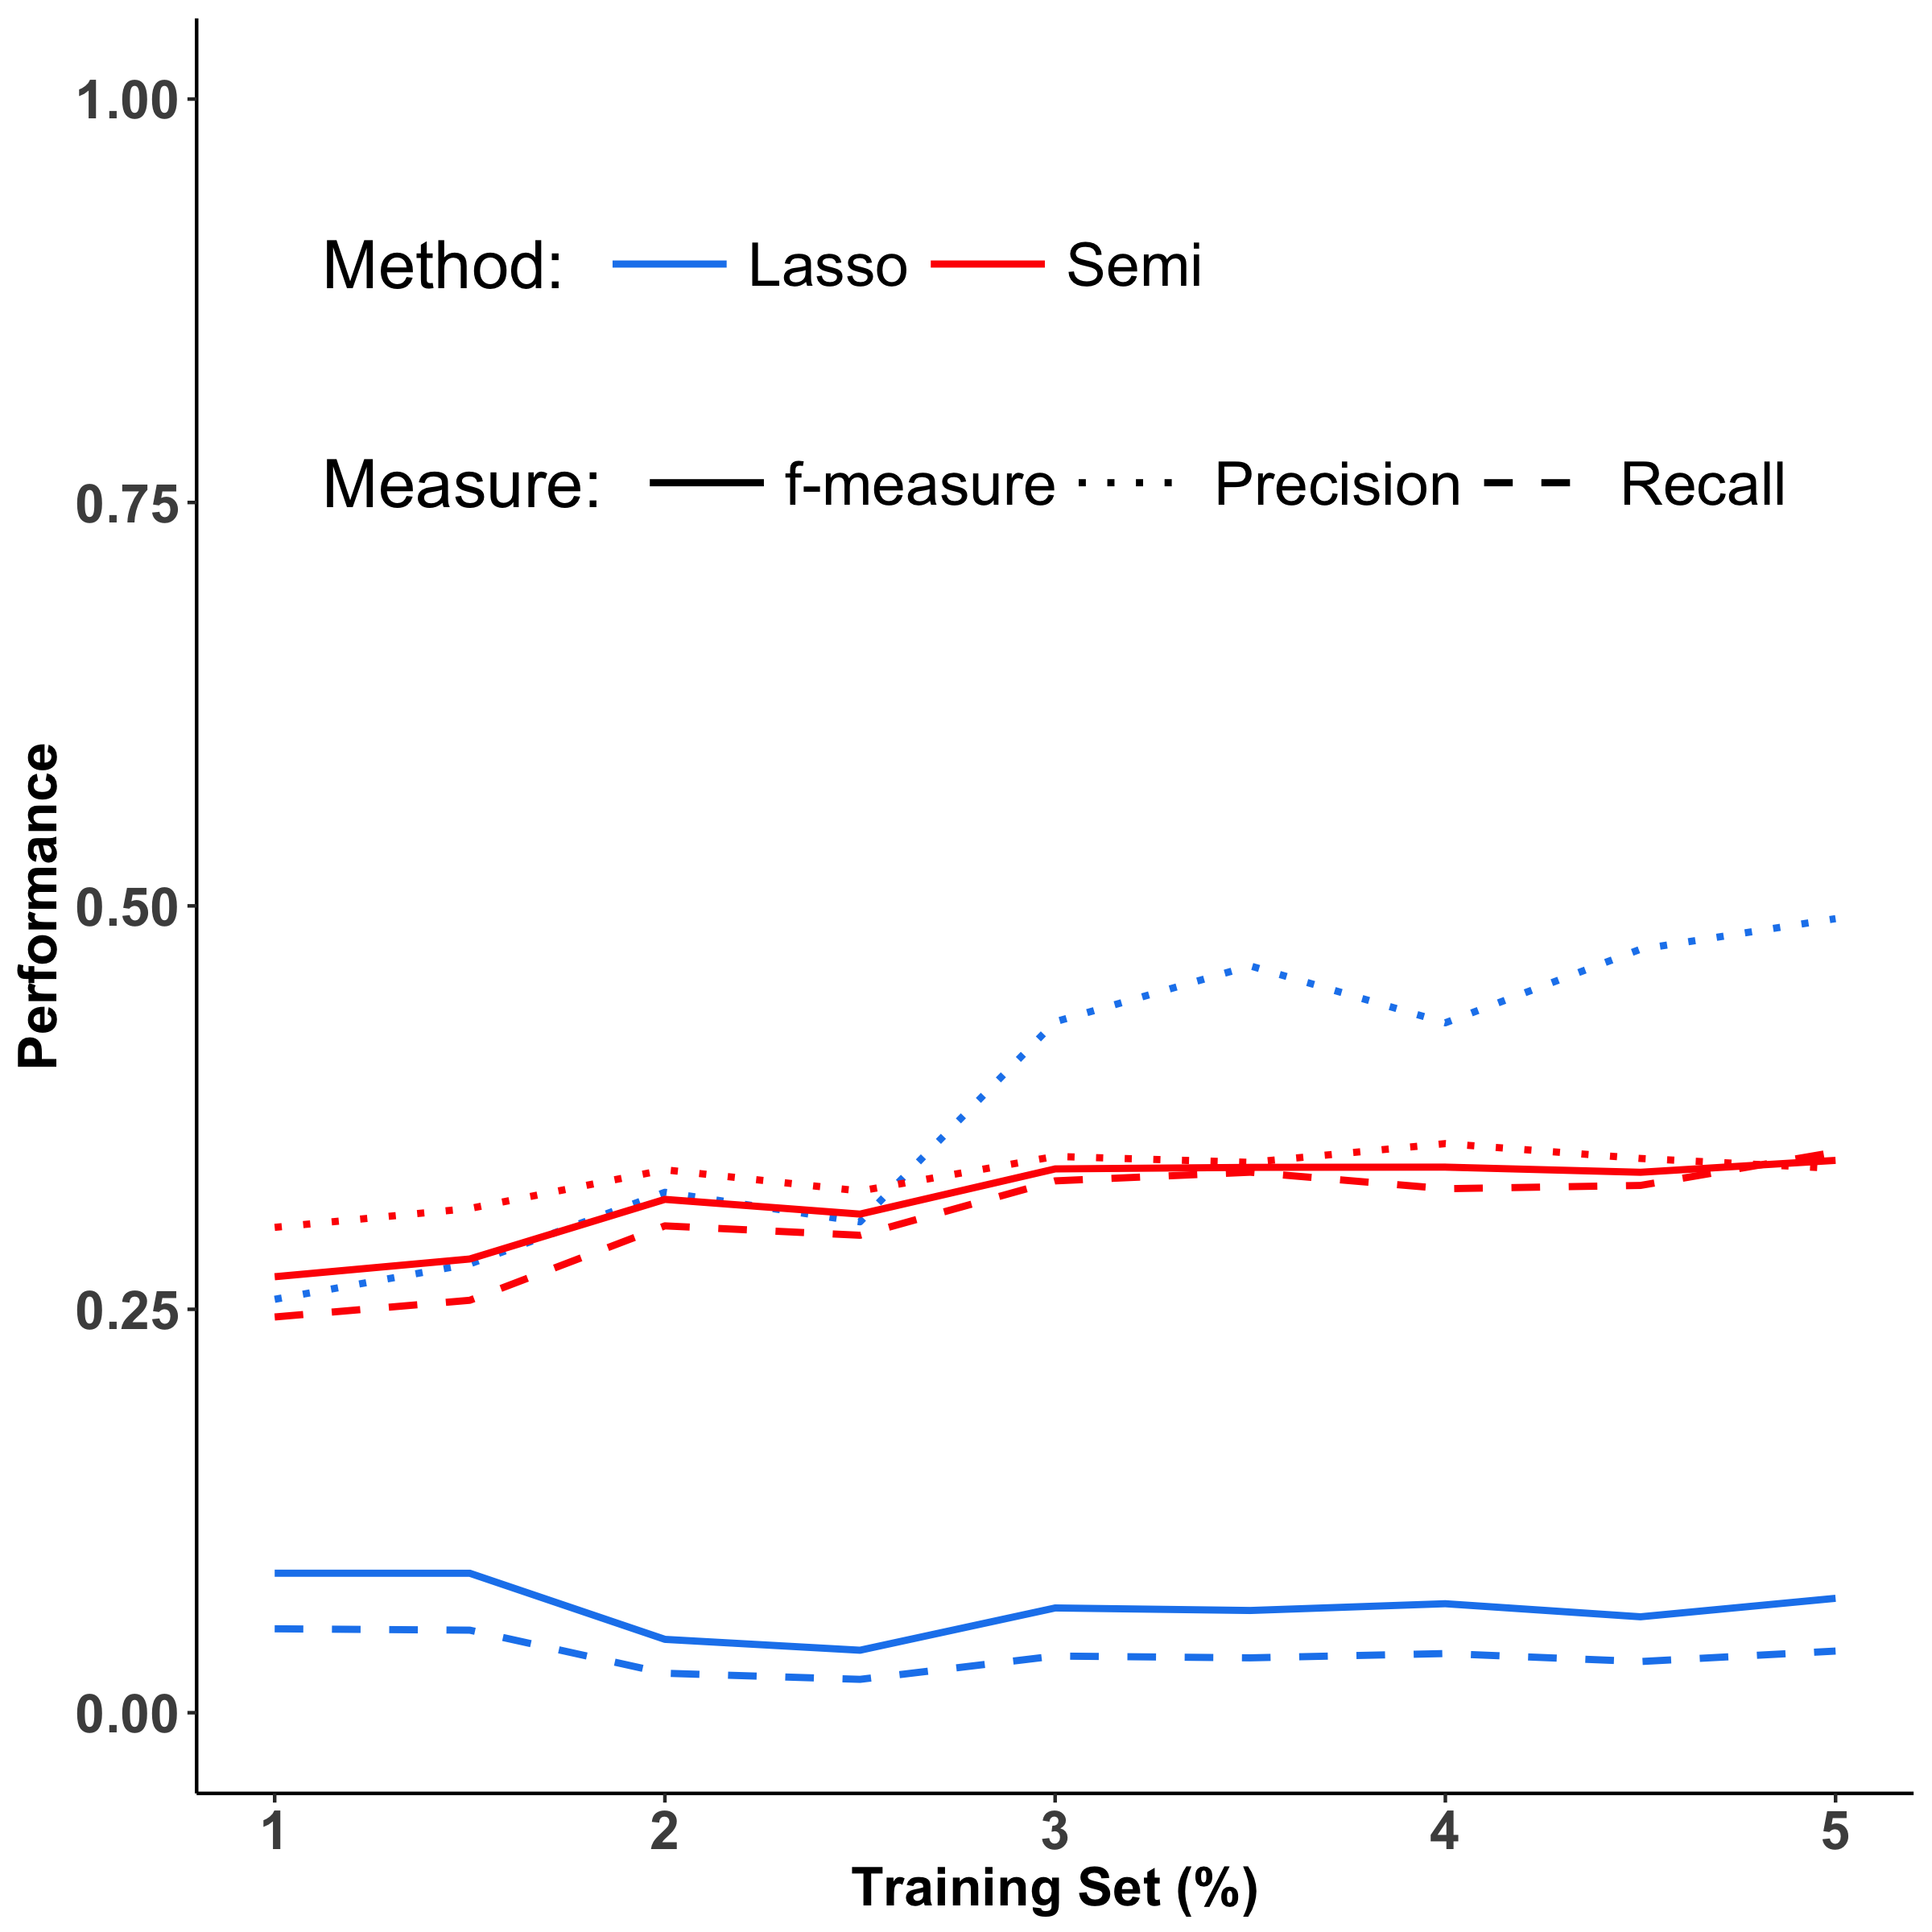
\includegraphics[width=\textwidth]{measures_pp95_20.png}
        \caption{0.95 Predicted Score Cutoff}
 %   \end{subfigure}
    \vspace{1cm}
    \caption{\textbf{Performance of Semi-supervised and LASSO methods with predicted score cutoffs at median, 0.50, 0.80, and 0.95 at 20\% contamination.} Semi-supervised method is shown in red while LASSO is shown in blue. Precision, recall, and f-measures are represented by dotted, dashed, and solid lines, respectively. The median is a relative cutoff while the other cutoffs represent absolute cutoffs with re-scaled predicted probabilities.}
    \label{fig:perf20}
\end{figure}


\begin{figure}[ht]
    \centering
%    \begin{subfigure}[b]{0.35\textwidth}
%        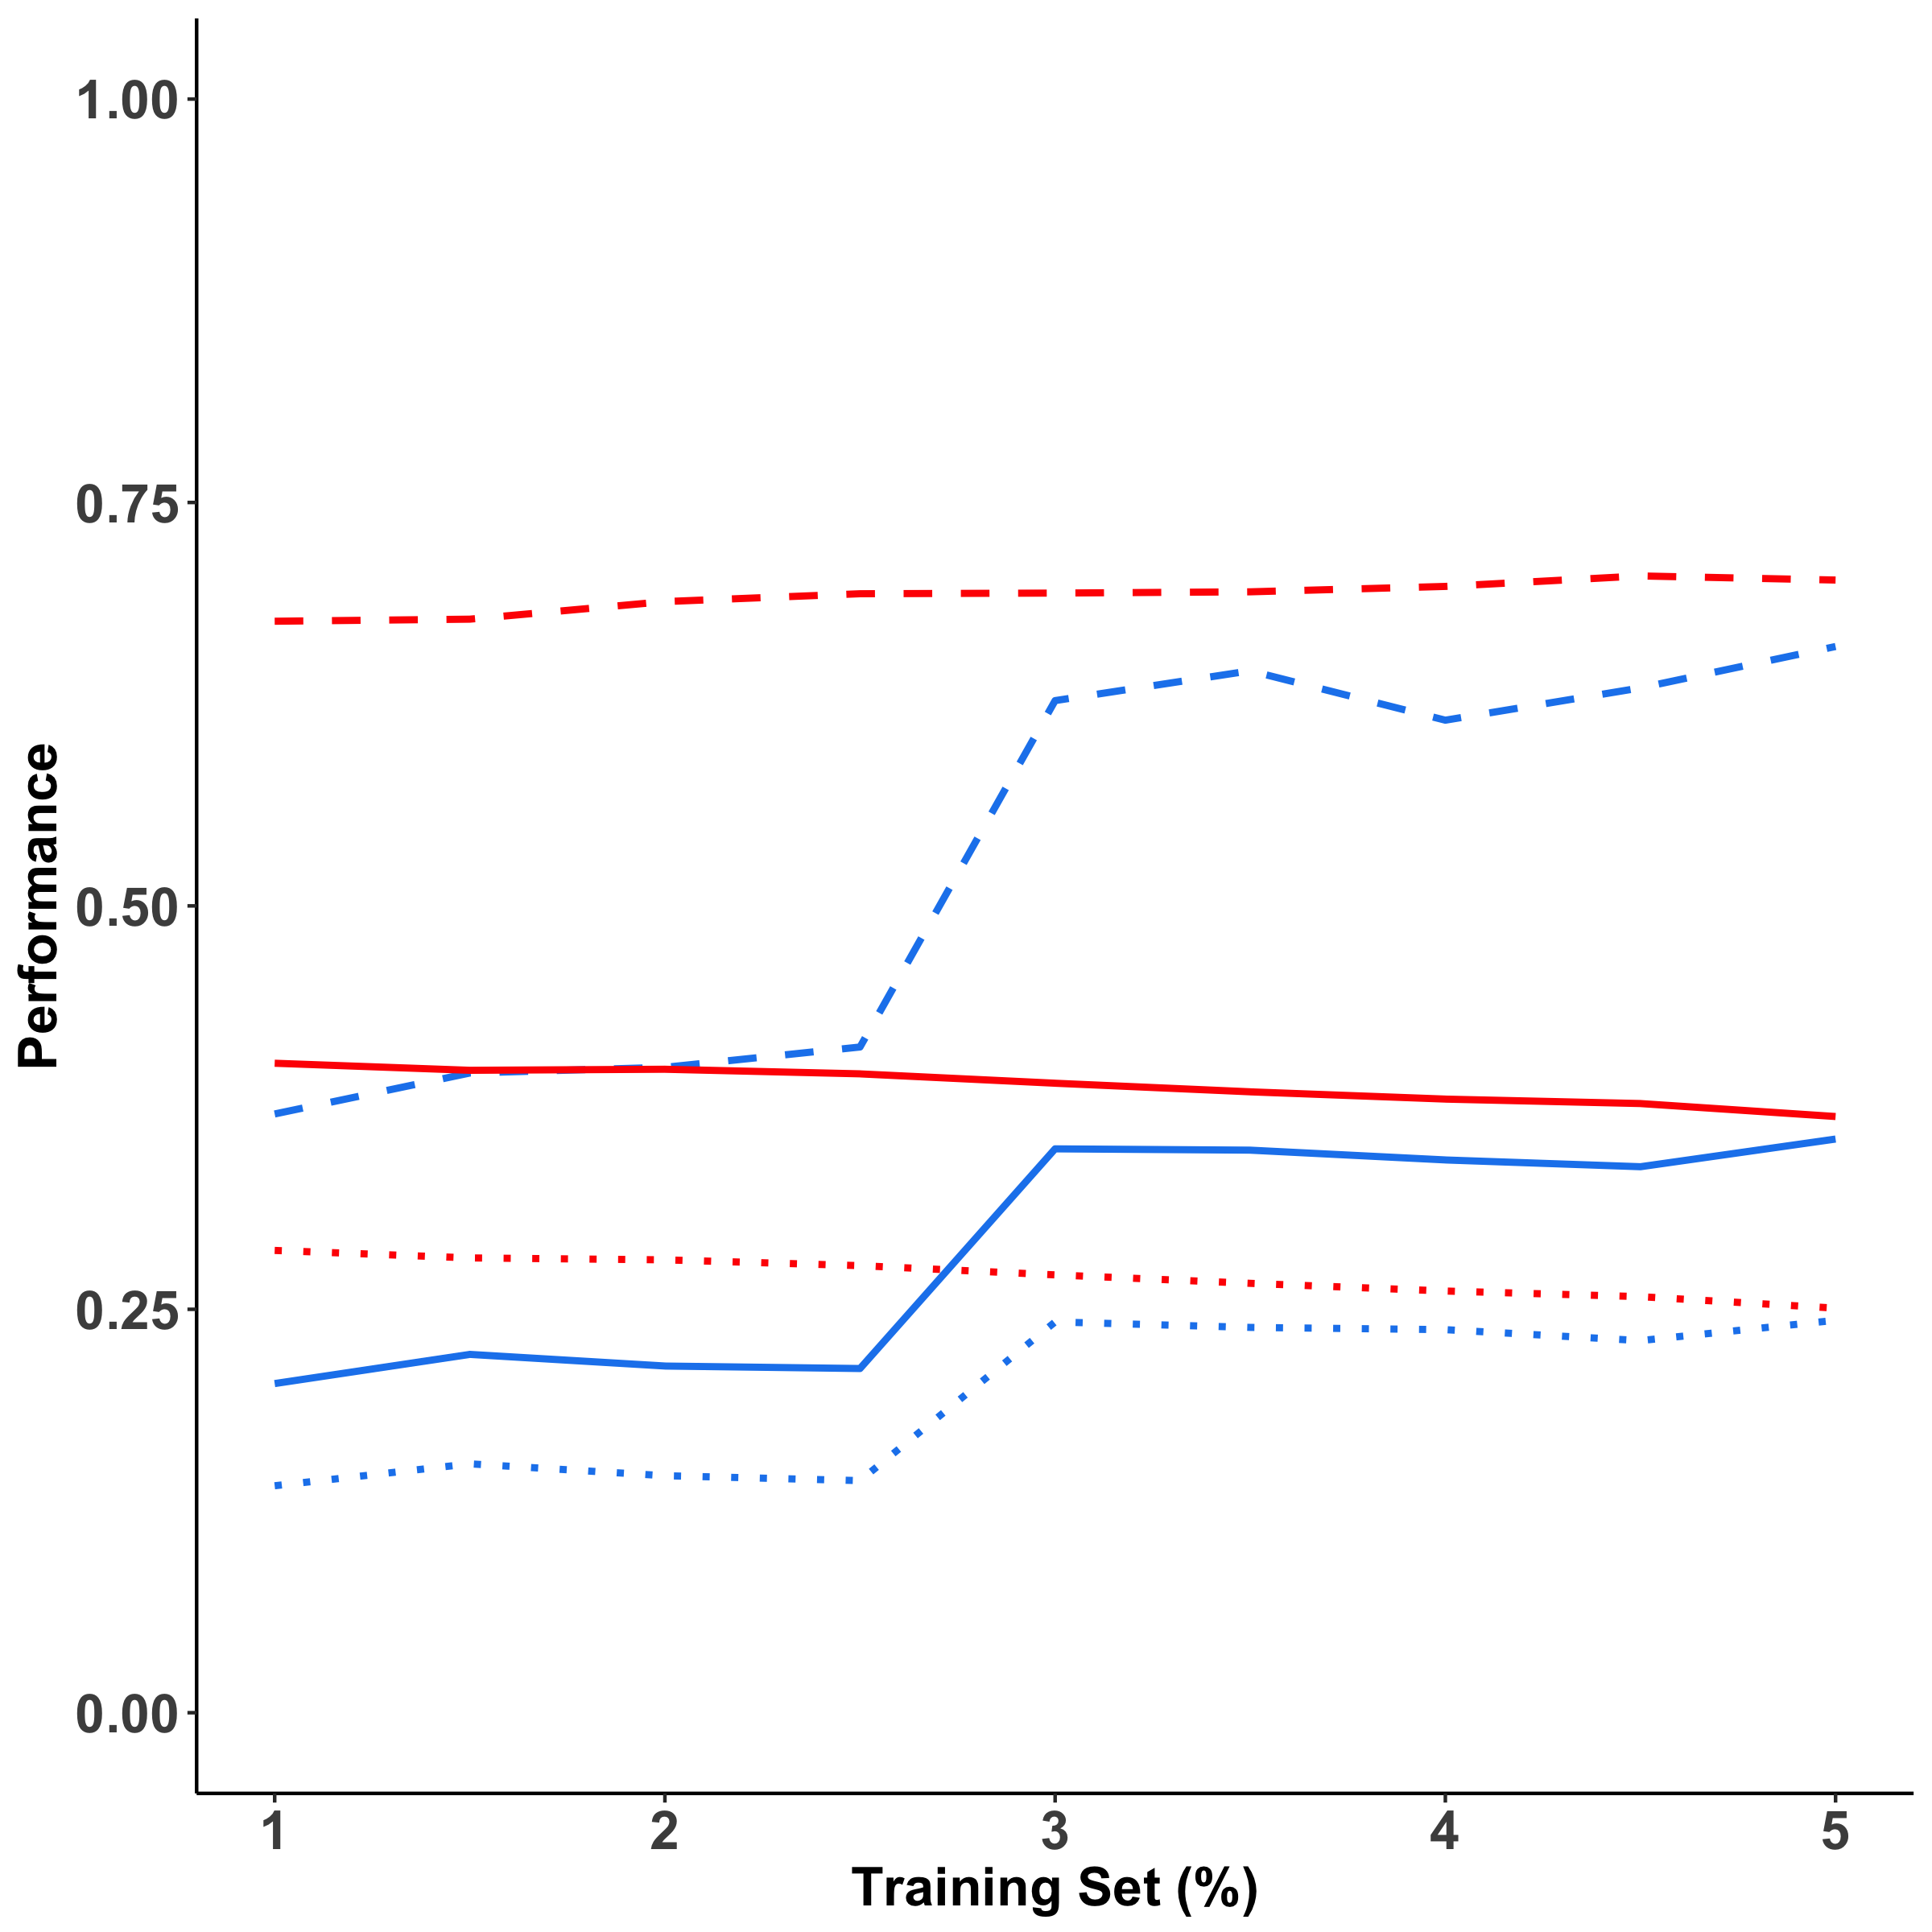
\includegraphics[width=\textwidth]{measures_median_50.png}
        \caption{Median Cutoff}
%    \end{subfigure}
%    \begin{subfigure}[b]{0.35\textwidth}
%        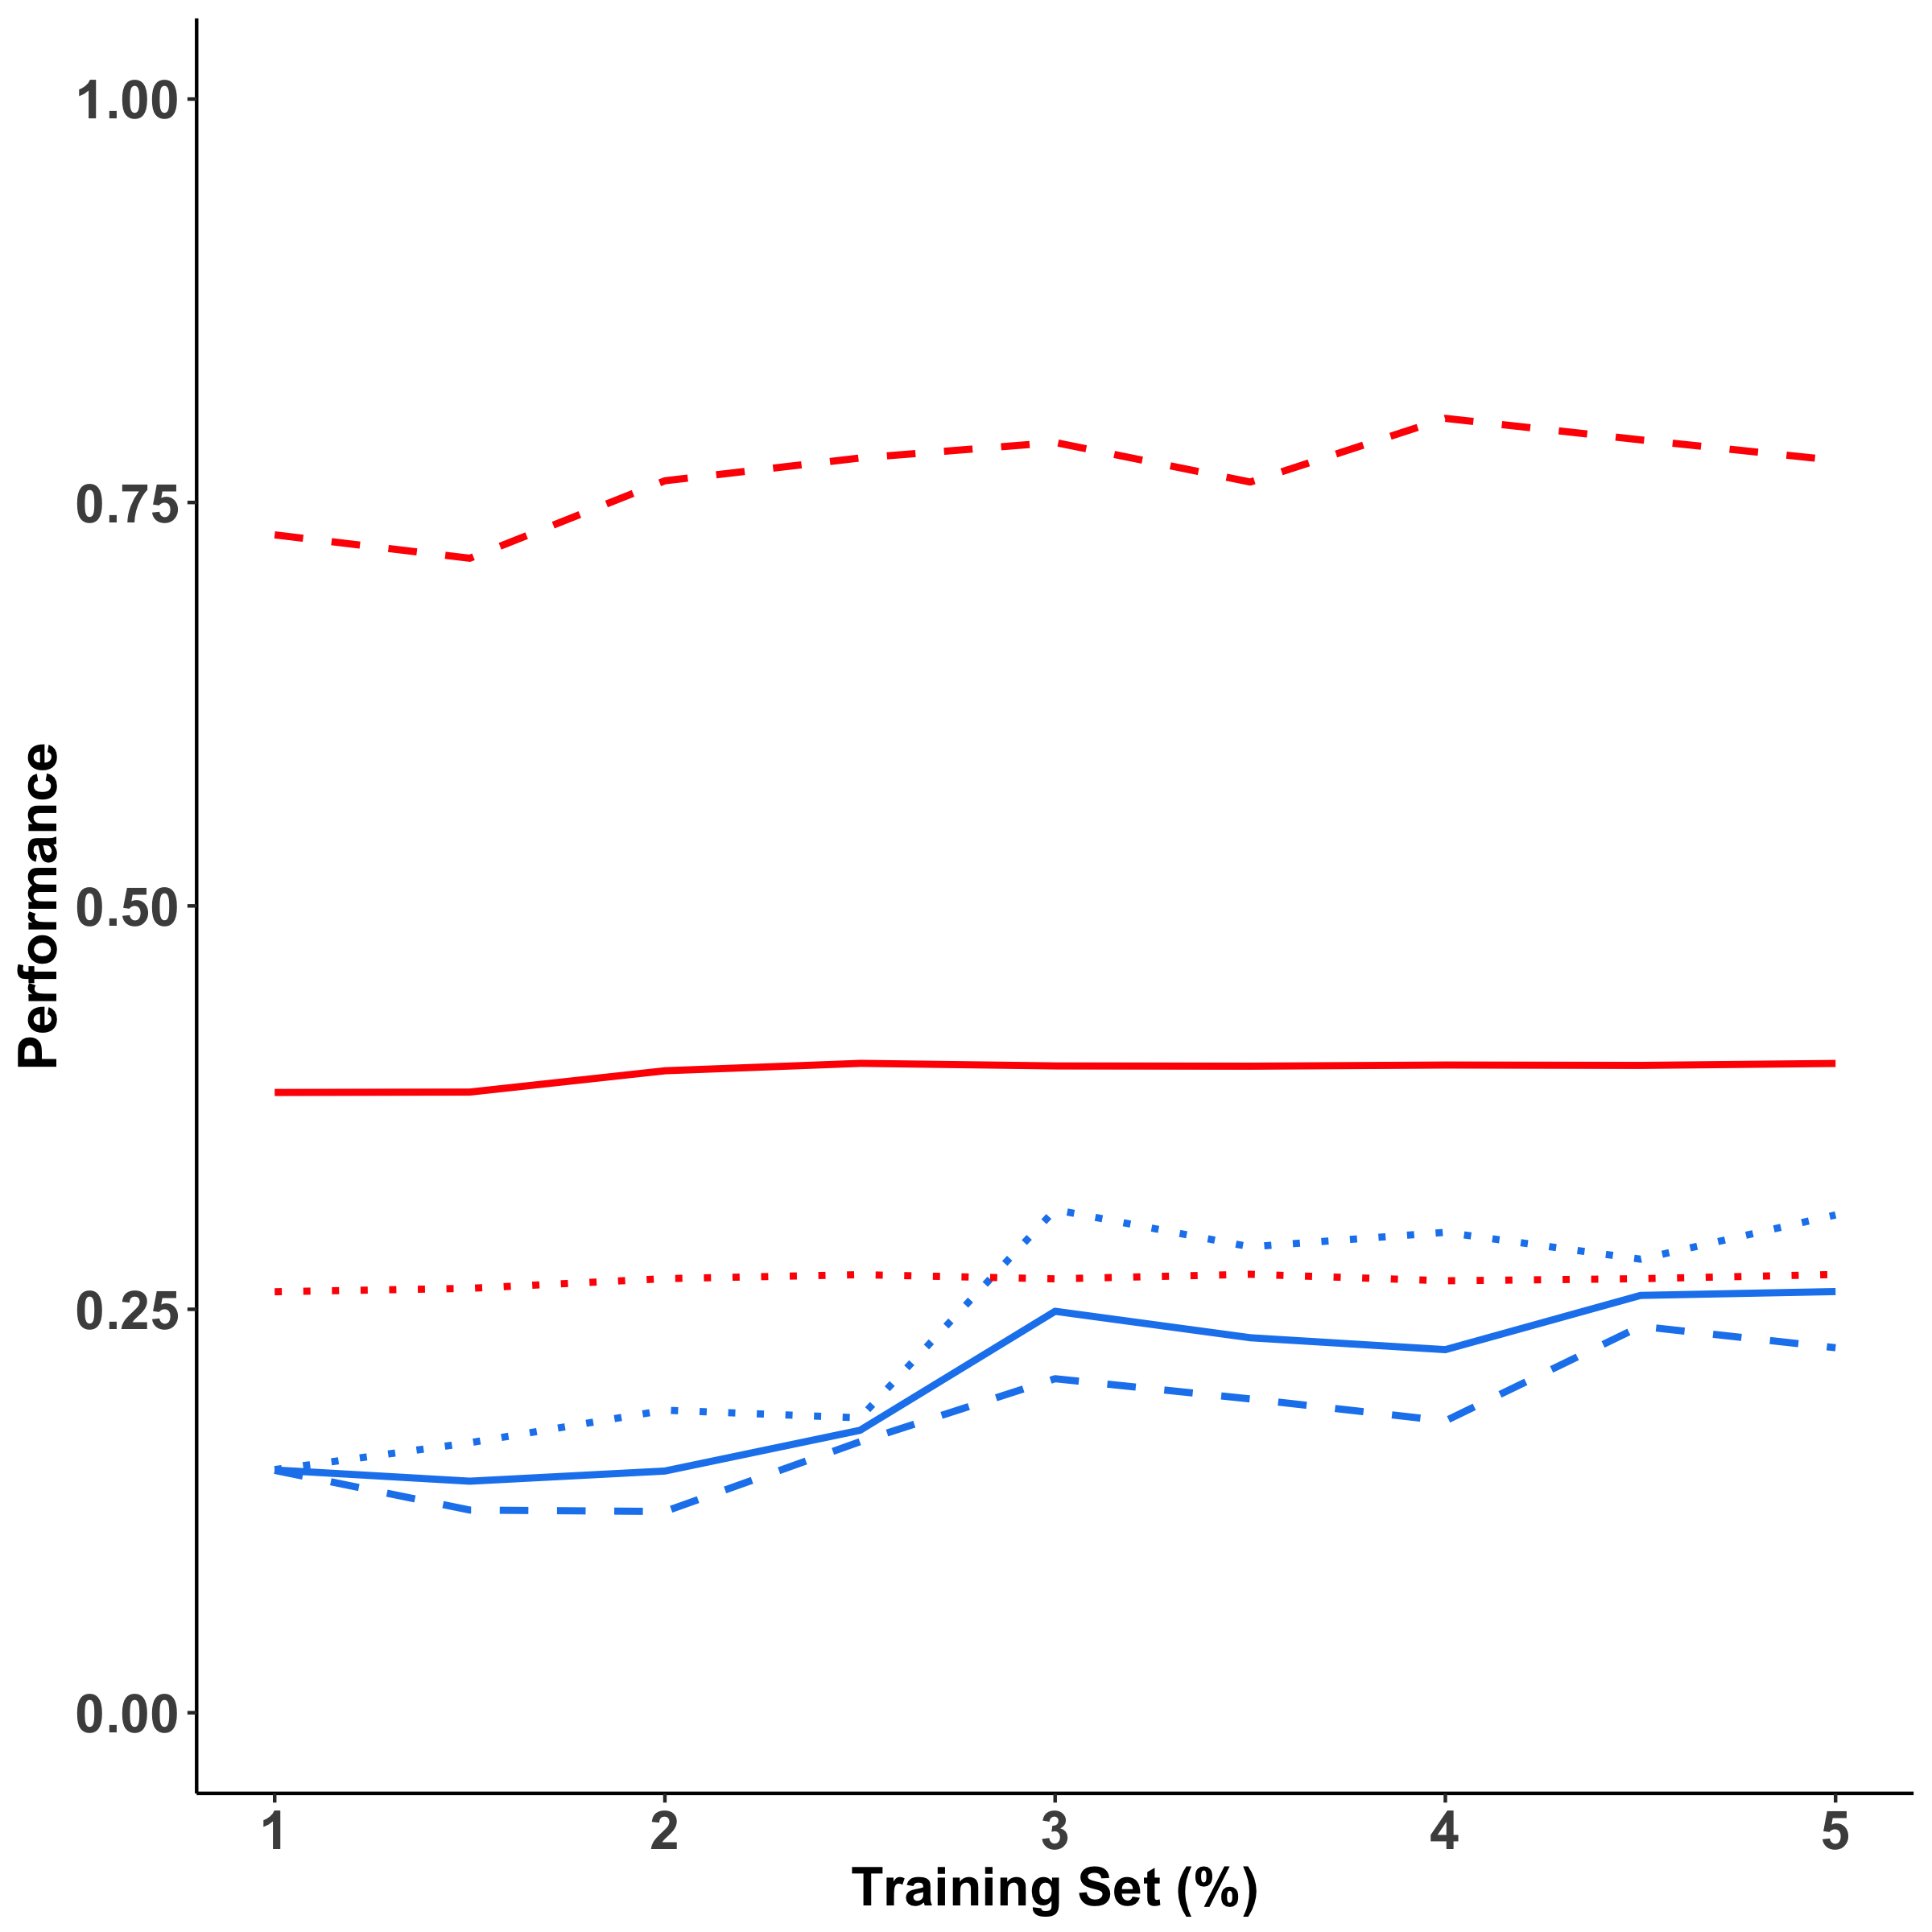
\includegraphics[width=\textwidth]{measures_pp50_50.png}
        \caption{0.50 Predicted Score Cutoff}
 %   \end{subfigure}
 %   \begin{subfigure}[b]{0.35\textwidth}
%        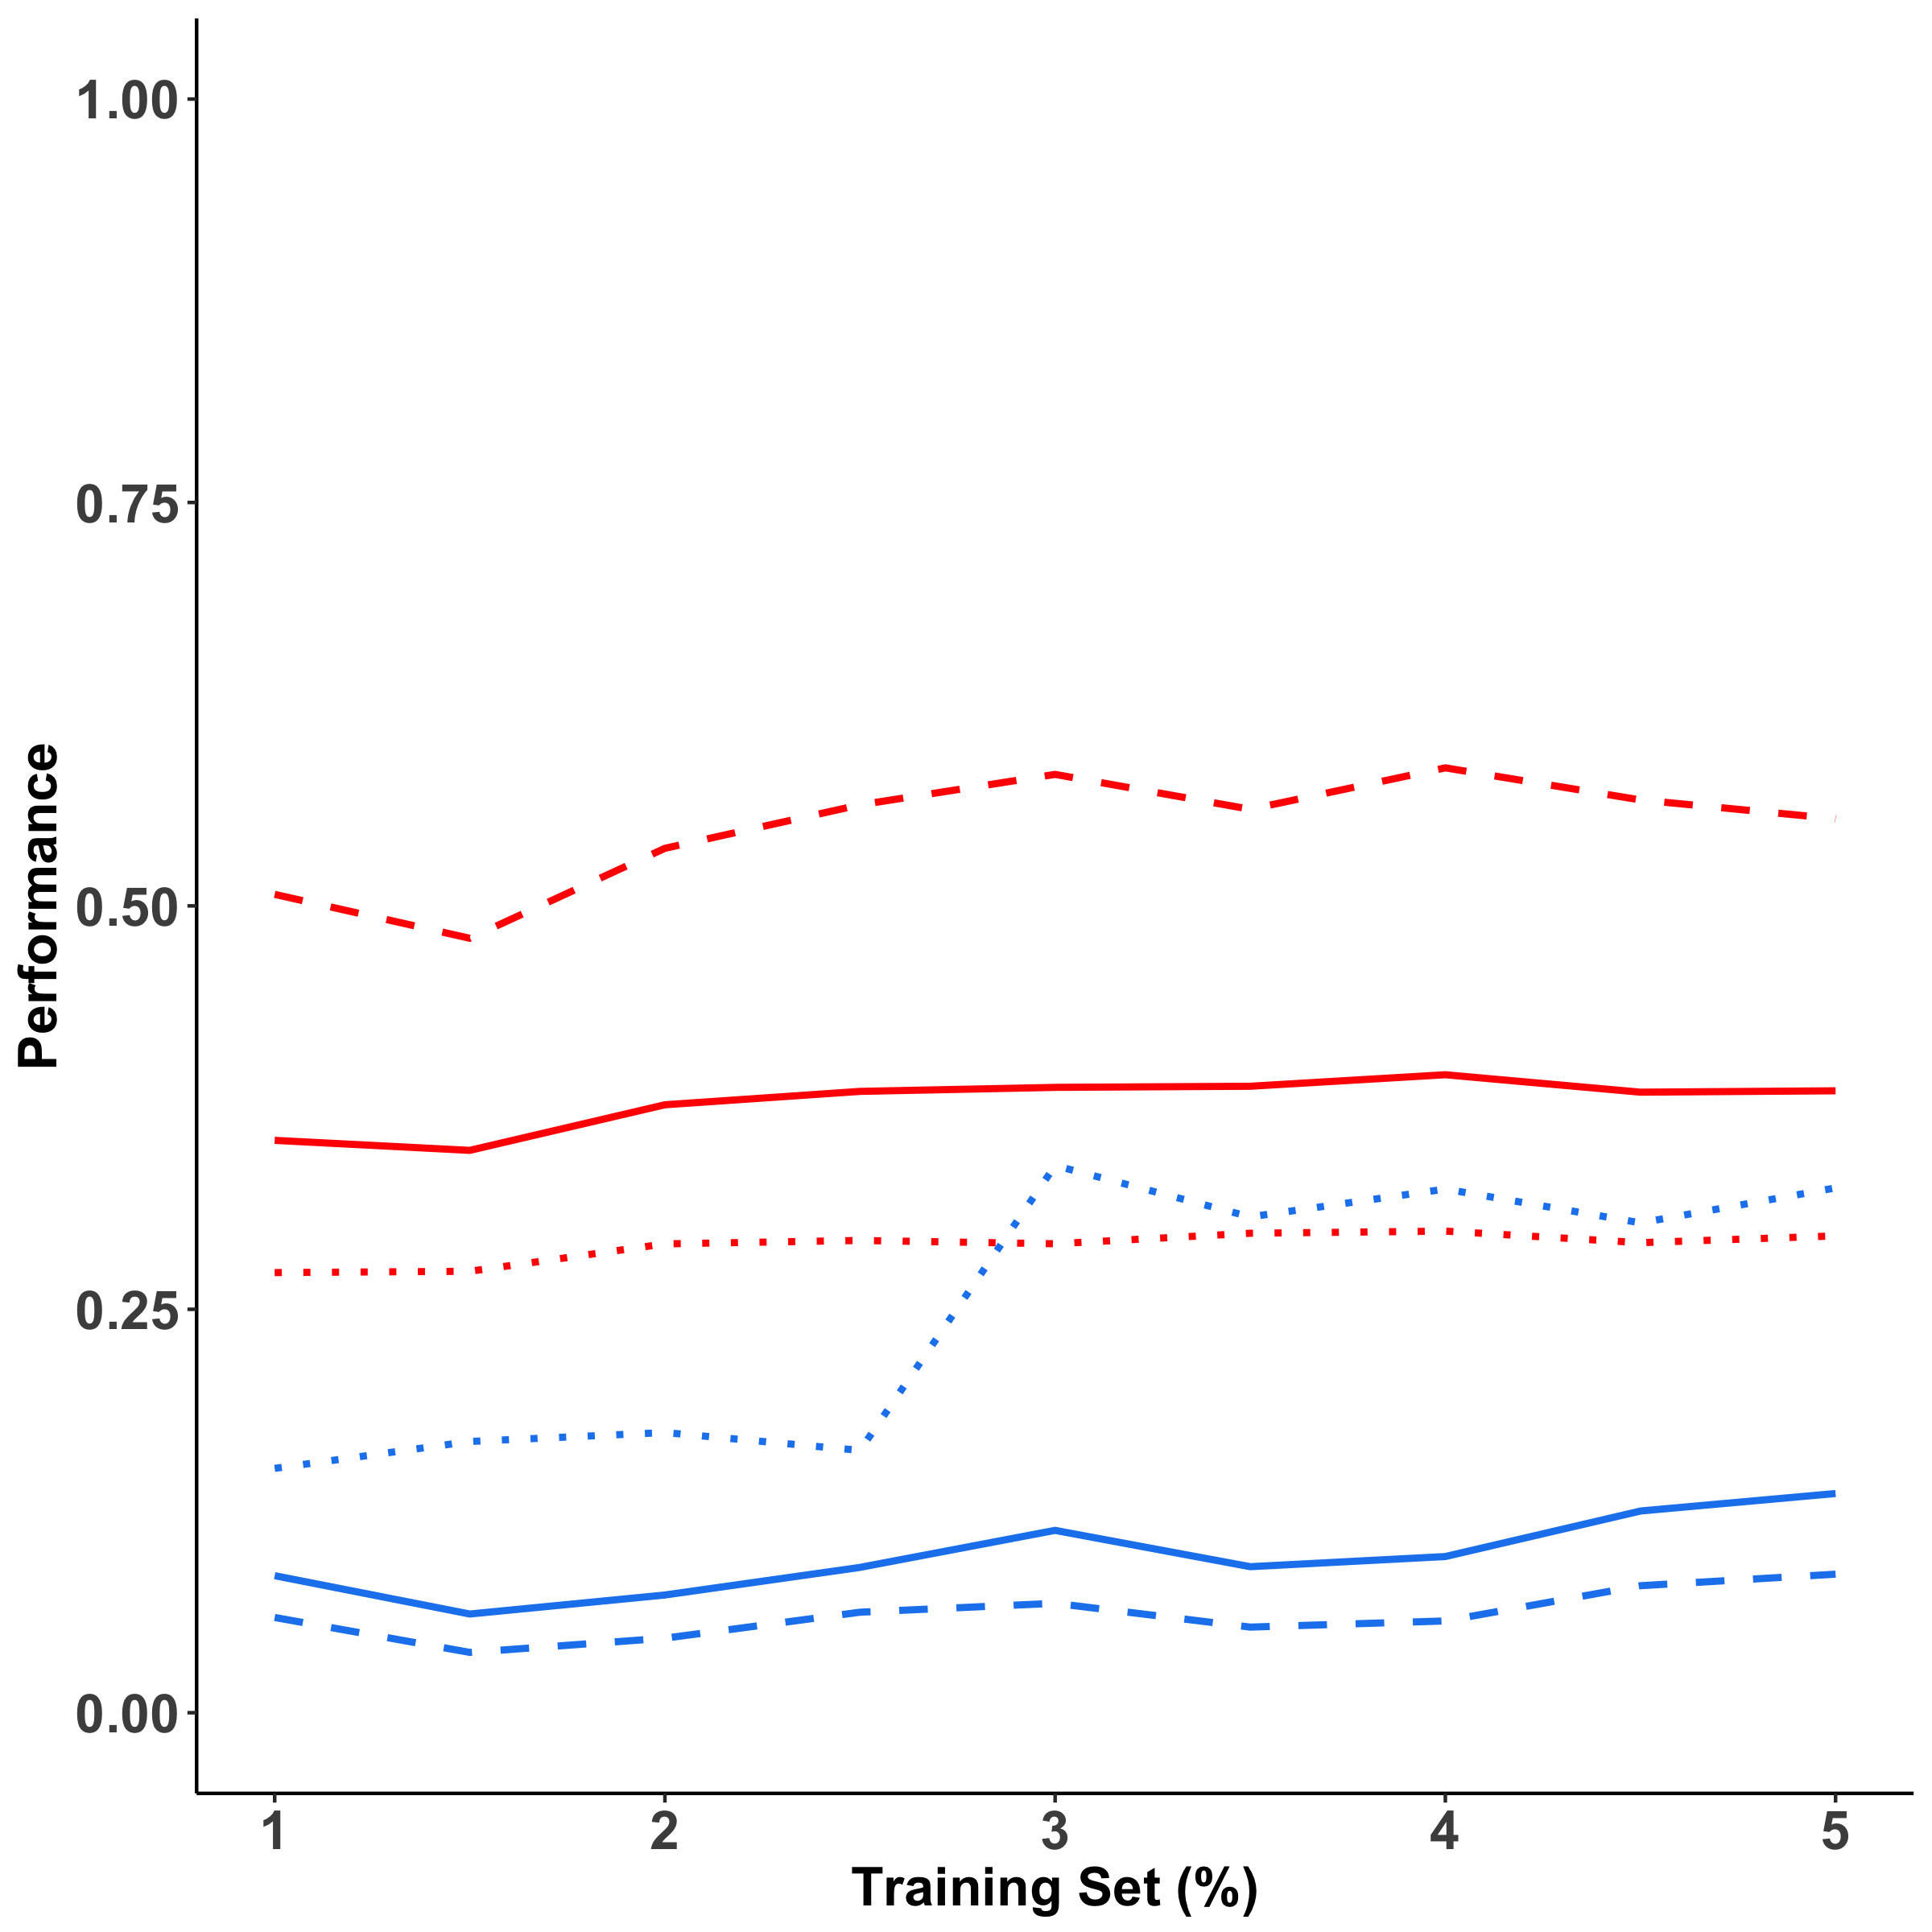
\includegraphics[width=\textwidth]{measures_pp80_50.png}
        \caption{0.80 Predicted Score Cutoff}
  %  \end{subfigure}
 %   \begin{subfigure}[b]{0.35\textwidth}
%        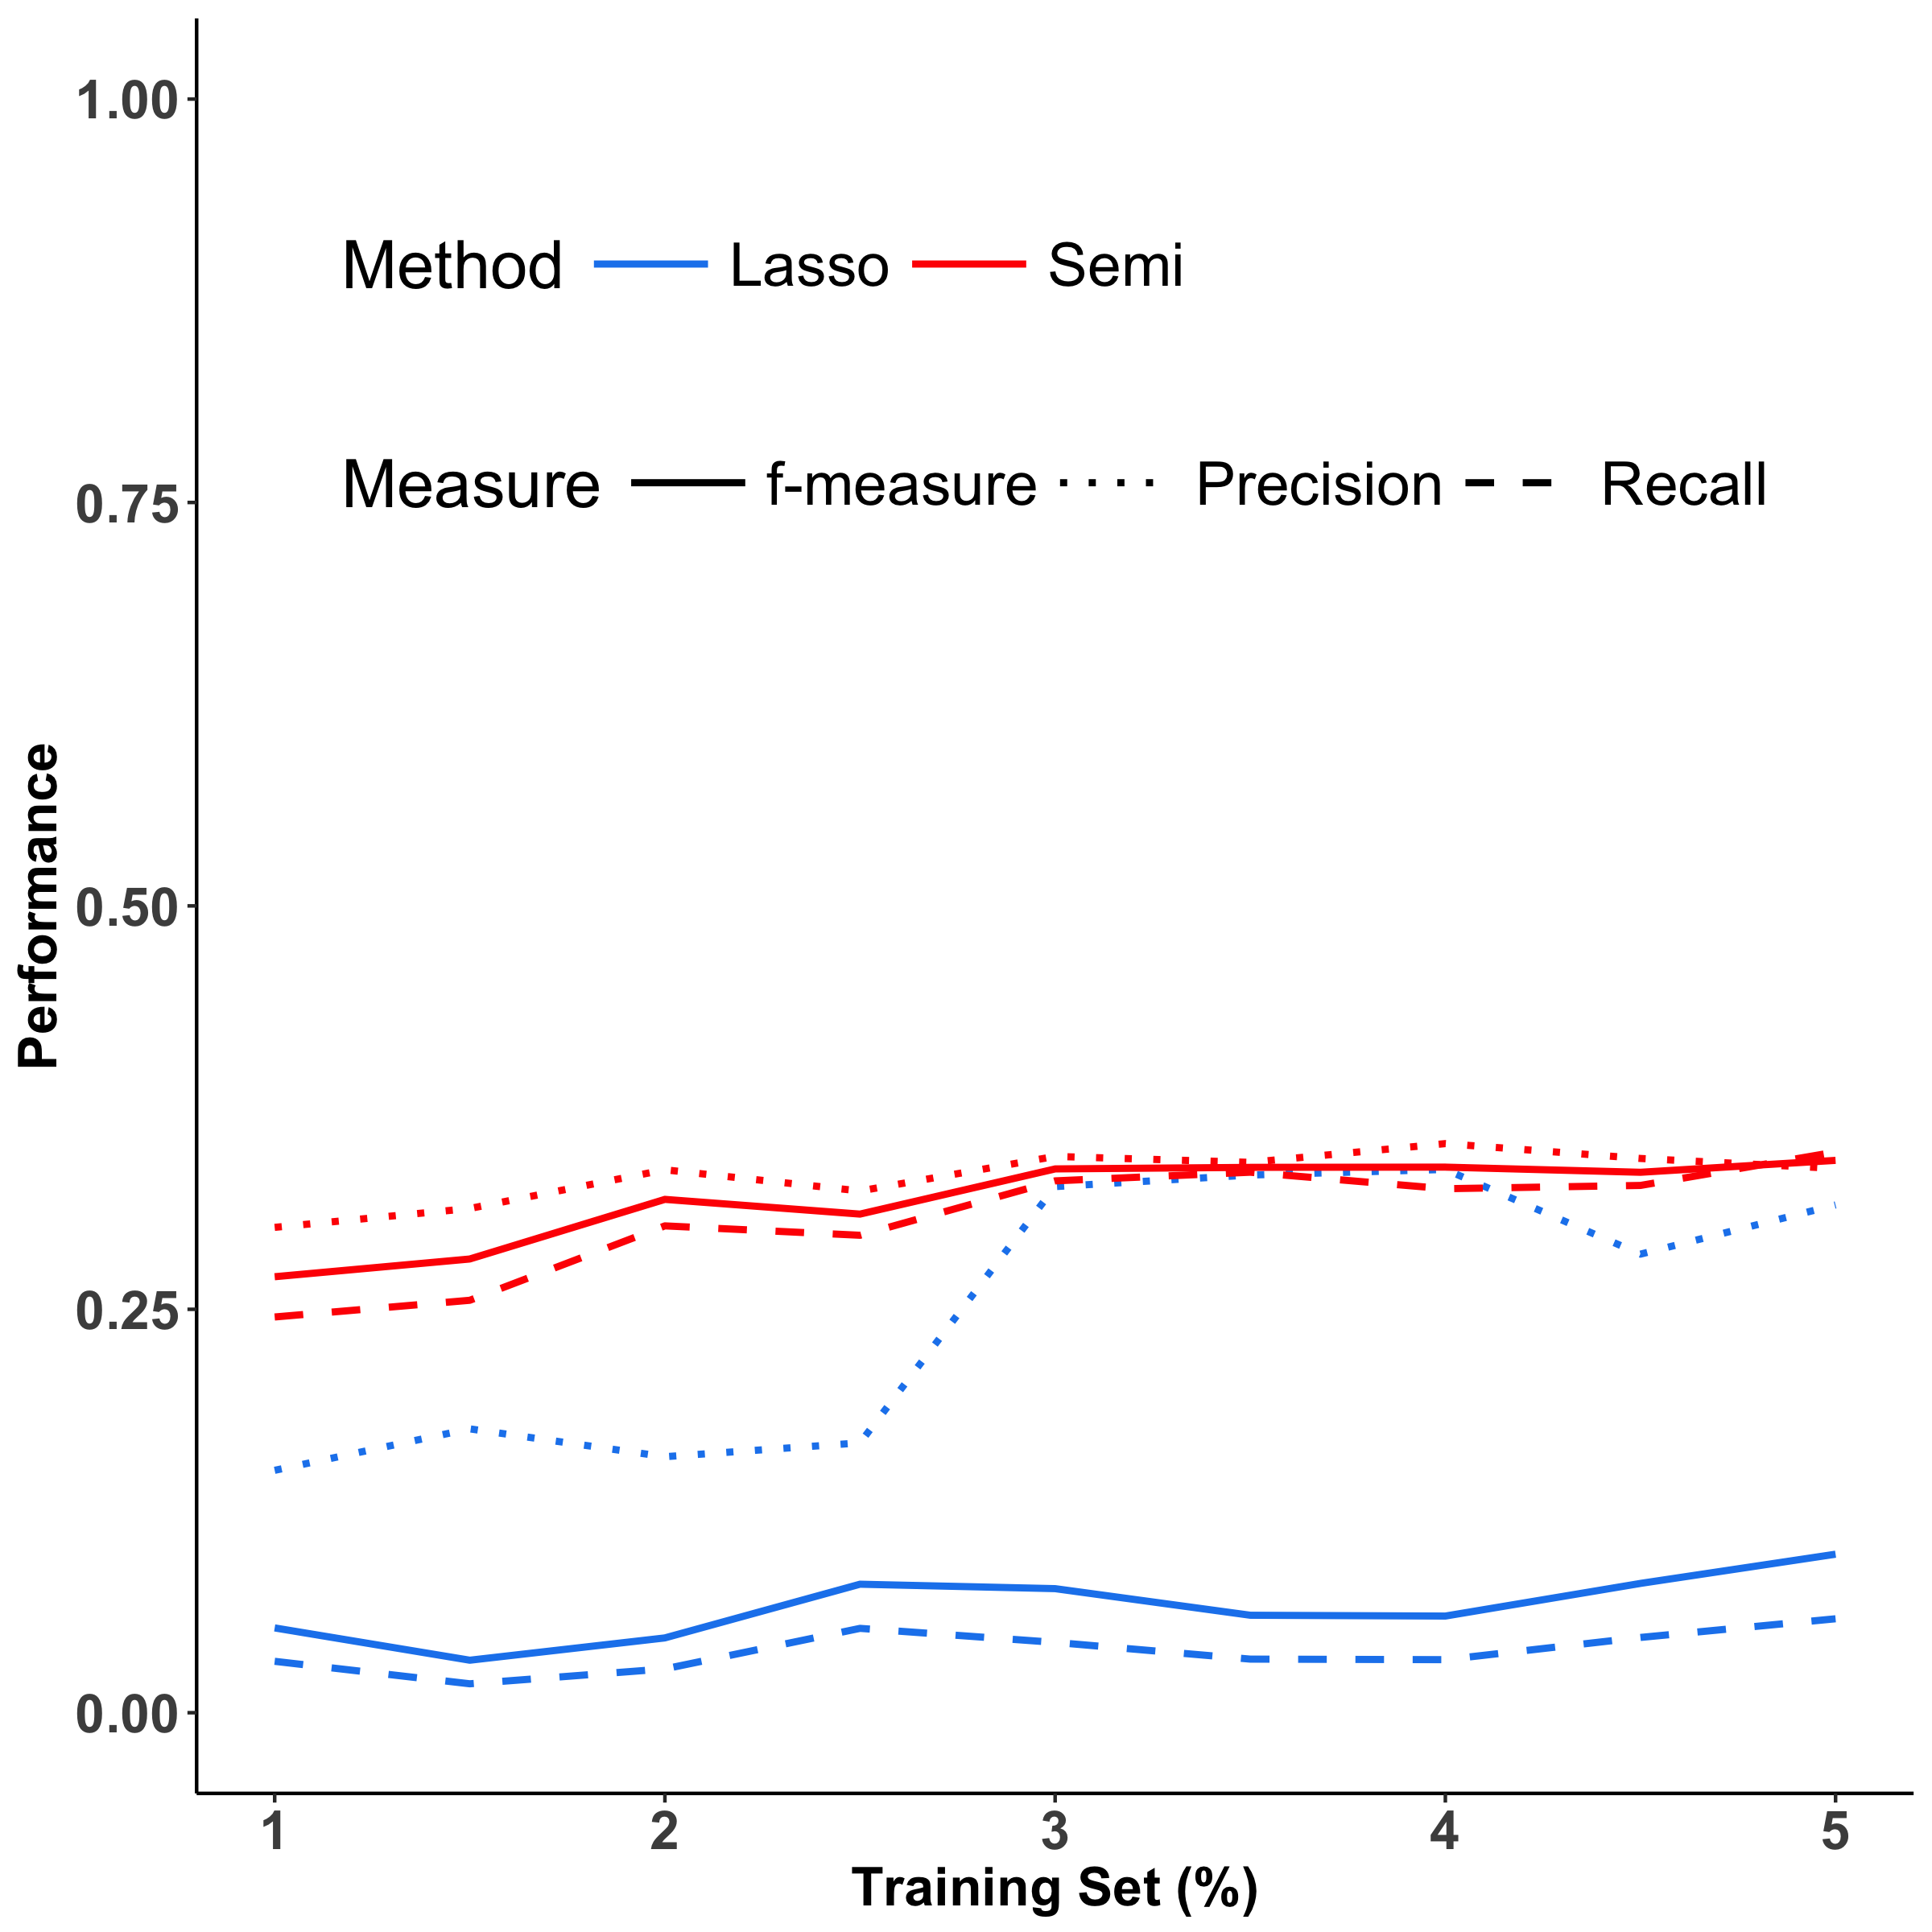
\includegraphics[width=\textwidth]{measures_pp95_50.png}
        \caption{0.95 Predicted Score Cutoff}
 %   \end{subfigure}
    \vspace{1cm}
    \caption{\textbf{Performance of Semi-supervised and LASSO methods with predicted score cutoffs at median, 0.50, 0.80, and 0.95 at 50\% contamination.} Semi-supervised method is shown in red while LASSO is shown in blue. Precision, recall, and f-measures are represented by dotted, dashed, and solid lines, respectively. The median is a relative cutoff while the other cutoffs represent absolute cutoffs with re-scaled predicted probabilities.}
    \label{fig:perf50}
\end{figure}

%%%%%%%%%%%%%%%%%%%%%%%%%%%%%%%%%%%
%%                               %%
%% Tables                        %%
%%                               %%
%%%%%%%%%%%%%%%%%%%%%%%%%%%%%%%%%%%

%% Use of \listoftables is discouraged.
%%
\section*{Tables}

\begin{table}[ht!]
\centering
\caption{Feature Definitions.\label{tab:methods.training.variables}}
\begin{tabular}{p{0.3cm} l p{8cm} c c c}
& \textbf{Abbreviation} & \textbf{Description} & \textbf{Type} & \textbf{Family} & \textbf{K}         \\
\hline
& cytoplasm     & Predicted subcellular location: cytoplasm             &	binary       &	bernoulli & 2 \\
& er            & Predicted subcellular location: er                    &	binary       &	bernoulli & 2 \\
& mitochondria  & Predicted subcellular location: mitochondria          &	binary       &	bernoulli & 2 \\
& nucleus       & Predicted subcellular location: nucleus               &	binary       &	bernoulli & 2 \\
& vacuole       & Predicted subcellular location: vacuole               &	binary       &	bernoulli & 2 \\
& other         & Predicted subcellular location: other                 &	binary       &	bernoulli & 2 \\
& tm helix      & Number of predicted transmembrane helices             &	integer      &  neg bin   & 2 \\
& cai           & Codon adaptation index                                &	[real]       &	gamma     & 2 \\
\raisebox{\dimexpr \measureISpecification}[0cm][0cm]{\rotatebox[origin=c]{90}{\small \textbf{Sequence Derived Features} }} & l aa & Length of putative protein in amino acid  &	integer      &	neg bin & 3   \\
& nc            & Effective number of codons                            &	(real)       &	normal    & 2 \\
& gravy         & Hydrophobicity                                        &	(real)       &	normal    & 2 \\
& gc            & \% GC content                                         &	[real]       &	gamma     & 2 \\
& close ratio   & \% codons one-third base pairs from stop codon        &	[real]       &	gamma     & 2 \\
& rare aa ratio & \% of rare aa in translated ORF                       &	[real]       &	gamma     & 2 \\
\hspace{0.25cm} \\
\hline
\hspace{0.25cm} \\
& intxn partners & Number of interaction proteins                       &	integer      &	neg bin   & 3 \\
& 6 yeast blast  & Number of related genes in 6 species of yeast        &	integer      &	poisson   & 2 \\
& blast yeast    & Number of related genes in yeast BLAST               &	integer      &	neg bin   & 2 \\
& dovexpr        & Dov Expression                                       &	(real)       &	pearson   & 3 \\
& chromosome     & Chr number                                           &	integer      &	poisson   & 2 \\
\raisebox{\dimexpr \measureISpecification}[0pt][0pt]{\rotatebox[origin=c]{90}{\small \textbf{Additional Features}}} & chr position & Chr position as \% of chromosome length                      &	[real]       &	gamma     & 2 \\
& 5 proks blast  & Number of related genes in 5 prokaryotes BLAST       &	integer      &	poisson   & 2 \\
& intron  & Contains an intron in DNA/RNA sequence                      &	binary       &	bernoulli & 2 \\

\end{tabular}
\vspace{0.5cm}
\caption{\textbf{Description of Features.} The sequence-derived features were compiled by Seringhaus \citep{Seringhaus2006a}. Additional features were assembled from the Gerstein labs \citep{GersteinLab}. Dov expression is the normalized difference between absolute mRNA expression levels \citep{Jansen2002}. Closed and open brackets indicate closed and open sets, respectively, under the \textbf{Type} heading. \textbf{Family} describes the distribution the marginal models utilized in the semi-supervised method. Note: chr position is labeled gamma which is a special case of the beta distribution. \textbf{K} is the calculated univariate optimized number of predicted classes for each variable.}
\label{tab:definition}
\end{table}

%%%%%%%%%%%%%%%%%%%%%%%%%%%%%%%%%%%
%%                               %%
%% Additional Files              %%
%%                               %%
%%%%%%%%%%%%%%%%%%%%%%%%%%%%%%%%%%%

\section*{Additional Files}
  \subsection*{Additional file 1 --- Sample additional file title}
   
   
\subsubsection*{Model Selection for Marginal Distribution $f$: ICL-BIC}
The BIC of \citep{Schwarz1978a}  is defined as $BIC= 2 \mathcal L_{X}(\hat\theta) - 
|\Theta| \log N$, with $\mathcal L_{X}(\hat\theta)$ being the log-likelihood of the estimated parameters given the 
observed data and $|\Theta|$ being the size of the parameter space. $ICL-BIC$ is defined as $ICL-BIC = 2 \mathcal L_{X, 
{\hat Y}}(\hat\theta) - |\Theta| \log N$, with $\hat Y$ being the maximum a posteriori (MAP) estimate of the value 
of the hidden data. Thus $ICL-BIC$ may be interpreted as the most probable value of $BIC$ if all data were observed.  All 
other things being equal, the model with the higher (often ``less negative'') $ICL-BIC$is preferred.  See \citep{Ji2005a} for 
an application of this criterion to models of gene expression, and \citep{Viroli2010a} for a comparison to other model 
selection criteria, where $ICL-BIC$ outperforms $AIC$ (Akaike's information criterion), $BIC$, and other criteria in selecting the correct mixture model.
   
 \subsubsection*{Selection of Weights $w^{trn}$}
The modeling of the observed data is the same as in the unsupervised case. By default, labeled samples are given the same 
weight as unlabeled samples in the parameter estimations.  However, if we  have a small training sample, we may choose to 
assign a higher weight $w^{trn}$ to labeled samples.   For further (M-step)  calculations involving the posterior probabilities 
calculated in Equation \eqref{eqn:methods.w_n_y_semisup_mixmod}, we  make the transformation $w_{n,y} \leftarrow w^{trn} 
w_{n,y}$ for each $n$ such that $t_n \leq K$, while leaving $w_{n,y}$  as-is for each $n$ such that $t_n = K^{trn}$.  The effective 
result of this is to add ``copies'' of the labeled samples to the  data set, thus increasing their influence on parameter estimation.  
For example, if we choose $w^{trn} = 2$, we are  effectively doubling the size of the training data.

Although values of $w^{trn} > 1$ often lead to better parameter estimates and therefore to better model predictions, 
overfitting can occur if $w^{trn}$ grows too large.  We use Monte Carlo cross-validation \citep{Shao1993a} to choose the 
best value from a list of candidate values, currently $w^{trn} \in \{1, 5, 10, 20, 50, 100\}$.  For a specified number of 
replications, currently 30, we sample without replacement half the training data, leaving the other half to serve as testing 
data for the current replication.  We then train the model with 
the first half of the data at each candidate weight, and calculate the receiver operating characteristic (ROC) area under the 
curve (AUC) for the trained models at each candidate weight.  The weight with the highest mean ROC-AUC across all 
replications is chosen as the final value of $w^{trn}$. \textbf{DD: THIS IS CROSS-VALIDATION WITH 1/1, TRY 2/1? What is used in the package?}


 \subsubsection*{EM Algorithm for Hierarchial Mixture Model}
Details for the estimation of parameters and conditional probabilities for the hidden variables are provided in this section. The unconditional status probability is $p_{0,y_0} = P(Y_0 = y_0)$, where $Y_0$ generates the distribution for the $Y_z$'s, and 
the component probability given the status is $q_{z,y_0,y_z} = P(Y_z = y_z | Y_0 = y_0)$.  Given observed data $\vec X = (\vec 
X_1, \ldots, \vec X_z)$ where $\vec X_z = (\vec x_{z,1}, \ldots, \vec x_{z,n})$, and parameters $\theta^{(i-1)}$, denote the 
conditional probabilities for the hidden variables by
\begin{equation}\label{eqn:weights_mdmixmod_defn}
	\begin{array}{rcl}
		u_{n,y_0} & = & P(y_{0,n} = y_0 | \vec x_{\cdot,n}, \theta^{(i-1)}), \\
		v_{z,y_0,n,y_z} & = & P(y_{0,n} = y_0, y_{z,n} = y_z | \vec x_{\cdot,n}, \theta^{(i-1)}) \text{ or} \\
		w_{z,n,y_z} & = & P(y_{z,n} = y_z | \vec x_{\cdot,n}, \theta^{(i-1)}).
	\end{array}
\end{equation}
 Let $I(\mathcal P)$ denote the indicator function.  Then for $\vec X$ as above, and hidden data $\vec Y = (\vec y_1, \ldots, \vec 
 y_Z)$ where $\vec y_z = (y_{z,1}, \ldots, y_{z,n})$ with $\vec y_0 = (y_{0,1}, \ldots, y_{0,n})$, the complete data log-likelihood is
\begin{equation}\label{eqn:mdmixmod_llik}
	\begin{array}{rcl}
		\mathcal L_{X, Y, y_0}(\theta) & = & \sum_{n, k_0} I(y_{0,n}=k_0) \log p_{0,k_0} \\
		& & + \sum_{n, z, (k) ,k_z} (I) \log q_{z,(k),k_z} \\
		& & + \sum_{n, z, k_z} I(y_{z,n}=k_z) \log f_{k_z}(x_{z,n} | \theta).
	\end{array}
\end{equation}
where $(k)$ denotes $k_0$ and $(I)$ denotes $I(y_{0,n}=k_0,y_{z,n}=k_z)$.  The Q-function is thus
\begin{equation}\label{eqn:mdmixmod_qfun}
	\begin{array}{rcl}
		 Q(\theta|\theta^{(i-1)}) & = & \sum_{n,k_0} u_{n,k_0} \log p_{0,k_0} \\
		& & + \sum_{n,z,(k),k_z} v_{z,(k),n,k_z} \log q_{z,(k),k_z} \\
		& & + \sum_{n,z,k_z} w_{z,n,k_z} \log f_{k_z}(\vec x_{z,n} | \theta^{(i-1)}).
	\end{array}
\end{equation}

The first step in joint model fitting is to fit a single mixture model to each data source, as described in Section 
\ref{subsec:methods.unsup.marginal}, to choose the number of components $K_z$ and marginal distribution which will be used 
for that data. Then the initialization, execution, and output of the EM algorithm as adapted for the model topologies are as 
follows:
\begin{enumerate}
	\item\label{em.overview.model.selection} Initialize the parameters for the hierarchical model based on the selected individual 
	mixture models.  Note that the individual model fits are used for initialization only, and do not imply any hard categorization of 
	the observed data before fitting the hierachical model.  
	\item\label{em.overview.estep} E-step:  for the $i$th iteration, using the previous iteration's parameter estimates $
	\theta^{(i-1)}$, estimate the conditional probabilities defined in Equation \eqref{eqn:weights_mdmixmod_defn}, which are
	\begin{equation}\label{eqn:layered_uvw}
		\begin{array}{rcl}
			u_{n, y_0} & = & \frac{p_{y_0}^{(i-1)} \prod_z \sum_{k_z} q_{z,y_0,k_z}^{(i-1)} g_{z,n,k_z}}{\sum_{k_0} p_{k_0}^{(i-1)} 
			\prod_z \sum_{k_z} q_{z,k_0,k_z}^{(i-1)} g_{z,n,k_z}}, \\
			v_{z,y_0,n,y_z} & = & u_{n,y_0} \frac{q_{y_0,y_z}^{(i-1)} g_{z,n,y_z}}{\sum_{k_z} q_{z,y_0,k_z}^{(i-1)} g_{z,n,k_z}}, \\
			w_{z,n,y_z} & = & \sum_{k_0} v_{z,k_0,n,y_z}
		\end{array}
	\end{equation}
	where $g_{z,n,y_z} = f_{y_z}(\vec x_{z,n} | \theta^{(i-1)})$.  
	\item\label{em.overview.mstep} 
	M-step:  estimate the current iteration's parameters, $\theta^{(i)} = \arg\max_\theta  Q(\theta |   \theta^{(i-1)})$.  
	This is a straightforward maximum likelihood estimation for the $p$'s and $q$'s, and a weighted MLE for the 
	parameters relating to the observed variables, using weights $\vec w_{z,\cdot,y_z}$ and data $\vec X_z$.
	\item\label{em.overview.iterate} Repeat steps\label{em.overview.iteration} \ref{em.overview.estep} and 
       \ref{em.overview.mstep} until convergence.
	\item\label{em.overview.report} Report the final estimated parameters $\hat\theta$ and posterior status probabilities $
	\vec{\hat U}$, the $N \times K_0$ matrix of which the $(n, y_0)$th element is $\hat u_{n,y_0} = P(y_{0,n} = y_0 | \vec x_n, \hat
	\theta)$.  Specifically, $\hat u_{n,1}$ is the estimated probability, given the data and the final estimated parameters, that the 
	$n$th gene is a gene of interest.
\end{enumerate}

  \subsection*{Additional file 2 --- Sample additional file title}
    Additional file descriptions text.


\end{backmatter}
\end{document}
